\documentclass[11pt]{amsart}

\usepackage[utf8]{inputenc}
\usepackage[T1]{fontenc}
\usepackage{lmodern}
\usepackage{amsmath, amssymb, amsthm, mathtools}
\usepackage{hyperref}
\usepackage{geometry}
\usepackage{booktabs}
\usepackage{graphicx}
\usepackage{enumitem}
\graphicspath{{figures/}}
\geometry{margin=1in}

\theoremstyle{plain}
\newtheorem{theorem}{Theorem}
\newtheorem{lemma}[theorem]{Lemma}
\newtheorem{proposition}[theorem]{Proposition}
\newtheorem{corollary}[theorem]{Corollary}

\theoremstyle{definition}
\newtheorem{definition}[theorem]{Definition}
\newtheorem{remark}[theorem]{Remark}

\newcommand{\R}{\mathbb{R}}
\newcommand{\eps}{\varepsilon}
\newcommand{\cG}{c_{G}}
\newcommand{\Astar}{A^{\star}}
\newcommand{\Hbody}{H_{\mathrm{body}}}
\newcommand{\Hworld}{H_{\mathrm{world}}}
\DeclareMathOperator{\area}{area}
\DeclareMathOperator{\trace}{tr}
\DeclareMathOperator{\diag}{diag}
\DeclareMathOperator{\Span}{span}

\title{Second-variation analysis for Gerver's sofa and\\
       Romik's ambidextrous candidate: finite-dimensional\\
       coercivity and a two-norm obstruction}
\author{Vico Bonfioli}
\date{\today}

\begin{document}

\begin{abstract}
We study the second variation of the moving-sofa area functional $F$
at Joseph Gerver's 1992 candidate sofa $\cG$, on the Sobolev space
$H^{2}([0,\pi/2];\R^{2})$ of corner trajectories modulo the
two-dimensional translation-symmetry quotient, and at Romik's
ambidextrous candidate $\Sigma$ $(A_{R}^{\star}\approx 1.64495)$.
Our conclusions are deliberately narrower than a local-maximality
statement, and we explain why.

We establish two things.  First, on the $16$-mode Fourier truncation
the computed $32\times32$ Hessian is negative definite, with
coercivity constant $m_{N}\geq 4.6035$ \emph{in the Euclidean
coefficient norm}, agreed on by three independent methods; this is a
genuine finite-dimensional strict-maximum statement, conditional only
on the floating-point polygon-intersection oracle.  Second, the
second variation is coercive in $H^{1}$, not in $H^{2}$: the diagonal
Rayleigh quotients $|Q[k,k]|/\|\varphi_{k}\|^{2}_{H^{1}}$ lie in
$[0.79, 1.24]$ for $k\leq 32$, whereas
$|Q[k,k]|/\|\varphi_{k}\|^{2}_{H^{2}}$ decays like $k^{-2}$, from
$0.366$ at $k=1$ to $1.9\times10^{-4}$ at $k=32$.  Since $Q[k,k] =
O(k^{2})$ while $\|\varphi_{k}\|_{H^{2}}^{2} = O(k^{4})$, \emph{no
positive uniform $H^{2}$ coercivity constant exists}.

Consequently the passage from the finite-dimensional computation to a
strict local maximum on $H^{2}$ is obstructed, and we do not claim it.
The obstruction is the classical two-norm discrepancy: $Q$ is coercive
only in $H^{1}$, while $F$ is defined only where the trajectory is
$C^{1}$, i.e.\ on $H^{2}\hookrightarrow C^{1}$; and the cubic
remainder carries a factor $\eta''$ (the Green's-theorem integrand is
linear in $c''$), so it cannot be dominated by the $H^{1}$ quadratic
term.  We state this openly as the principal obstruction rather than
absorbing it into a constant.  For $\cG$ the qualitative local
maximality is in any case a consequence of Baek's~\cite{Baek2024}
global resolution, not of the present analysis; for $\Sigma$, where no
such result is available, local maximality remains \emph{open}.

Two further non-rigorous ingredients are flagged throughout:
(i) the finite-dimensional Hessian is evaluated with a floating-point
polygon-intersection oracle rather than true interval arithmetic; and
(ii) the low-to-high mode cross-term is bounded by a numerical
placeholder rather than an analytic estimate.  The second variation
decomposes as $Q = Q_{\mathrm{smooth}} + Q_{\mathrm{jump}}$, where
Lemma~8 characterizes the smooth piece analytically and the jump piece
at the four contact-transition breakpoints is captured only
empirically; its rank is not determined by the diagonal.
The supporting computations are:
(i) a high-precision Newton enclosure of Gerver's analytic constants
matching Romik~\cite{Romik2018}'s published Table~1 values
(see Section~\ref{sec:phase1} for the precision discussion);
(ii) the finite-dimensional Hessian computation described above (the
$128$-bit interval step encloses the finite-difference
step-sensitivity between step sizes, \emph{not} the floating-point
polygon-intersection error of caveat~(i), so this is a high-precision
computation rather than a certified enclosure of the true second
variation);
(iii) the symbolically-verified structural identity that the second
variation contains no $\|\eta''\|^{2}$ principal symbol, yielding the
$c_{G}$-independent growth bound
$|Q[k,k]| \leq (3\pi/2) k^{2} + (6\pi + 12) k$.  It is precisely this
$O(k^{2})$ growth, set against the $O(k^{4})$ growth of the
$H^{2}$-norm, that produces the obstruction described above; the same
bound shows the second variation is a \emph{bounded} operator of small
norm on $H^{2}$, so $\cG$ is close to degenerate in the
$H^{2}$ topology.
Phase~1 reconfirms Gerver's area
$\Astar = 2.219531668871967\ldots$ to the precision of
Romik~\cite{Romik2018}'s published Table~1
($\approx 16$~decimal digits).
The eigenvalue-growth bound is verified empirically across
$k \in \{1, 2, \ldots, 32\}$ with worst-case multiplicative margin
$\geq 1.35\times$ near $k = 14$ and asymptotic margin
$\geq 2.15\times$ at $k = 32$.
\end{abstract}

\maketitle

\section{Introduction}

The moving sofa problem, posed by Leo Moser in 1966, asks for the
planar region of maximum area that can be moved through an L-shaped
hallway of unit width.  The current best lower bound was constructed
by Joseph Gerver in 1992~\cite{Gerver1992}: an explicit
18-piece region with area
\begin{equation}\label{eq:Astar}
  \Astar \;=\; 2.219531668871967889\ldots,
\end{equation}
which Gerver conjectured to be optimal but did not prove.  The
strongest published upper bound prior to 2024, due to
Kallus--Romik~\cite{KallusRomik2018}, is approximately~$2.37$.  In
2024, Baek~\cite{Baek2024} resolved the conjecture, showing
$\mu^{\star} = \Astar$, so that Gerver's sofa is globally---and hence
locally---optimal.  Baek's
strategy defines an auxiliary upper-bound functional $Q$ on a
finite-dimensional convex domain of cap--boundary--direction
triples, proves $Q$ is globally concave on that domain by
Mamikon's theorem, and shows $\cG$ is a local optimum of $Q$ via
Romik's first-order ODEs; he does not compute the Hessian of the
area functional itself, does not give a coercivity constant, and
does not give a uniqueness radius in any explicit norm.  The
present paper takes a structurally different route: we work
directly with the second variation of the area functional $F$ in
a Sobolev framework.  By Baek's resolution, global maximality of
Gerver's sofa implies its local maximality, so we are not in doubt
about \emph{whether} $\cG$ is locally maximal; the question is
whether a second-variation argument can establish it
quantitatively.  Our answer is a qualified no, and the reason is
structural rather than computational.

On the $16$-mode truncation the computed Hessian is negative
definite, with $m_{N}\geq 4.6035$ in the Euclidean coefficient
norm---a genuine finite-dimensional strict-maximum statement,
conditional only on the polygon-intersection oracle.  But this
constant does \emph{not} transfer to the ambient space.  The second
variation satisfies $Q[k,k] = O(k^{2})$ (Theorem~\ref{thm:hypV}),
while $\|\varphi_{k}\|_{H^{2}}^{2} = O(k^{4})$, so the $H^{2}$
Rayleigh quotient decays to zero and no positive uniform $H^{2}$
coercivity constant exists.  What survives is coercivity in the
weaker norm $H^{1}$, where the two growth rates match.  The gap
between the norm in which the second variation is coercive
($H^{1}$) and the norm in which the functional is even defined
($H^{2}\hookrightarrow C^{1}$, needed to make sense of $c'$ in the
contact construction) is a two-norm discrepancy, and the cubic
remainder---which carries a factor $\eta''$---is not dominated by
the $H^{1}$ quadratic term.  We record this obstruction explicitly
in Section~\ref{sec:discussion} rather than absorbing it into a
constant.

The method applies verbatim to the \emph{ambidextrous} moving-sofa
problem, where Romik's candidate $\Sigma$~\cite{Romik2018} is
conjectured optimal but neither global nor local optimality is known
(Romik~\cite[\S7, Open Problem~1]{Romik2018}).  There
(Section~\ref{sec:romik}) we obtain the analogous finite-dimensional
negative-definiteness for $\Sigma$.  Because no global result is
available for $\Sigma$, and because the same two-norm obstruction
applies, local maximality of $\Sigma$ remains \emph{open}; we do not
claim it.

Romik~\cite{Romik2018} reformulated Gerver's solution as the rotation
path of the hallway's inner corner in the body frame of the sofa,
parameterized by an angle $\theta \in [0, \pi/2]$.  In this
formulation the candidate sofa is the body-frame intersection
\begin{equation}\label{eq:S_x}
  S(c) \;=\; \bigcap_{\theta \in [0, \pi/2]}
              R(+\theta)\, \Hworld + c(\theta),
\end{equation}
where $\Hworld$ is the fixed unit-width L-hallway, $R(\theta)$ is the
standard counter-clockwise rotation, and $c(\theta) = (c_x(\theta),
c_y(\theta))$ is the corner trajectory.  Romik gives $\cG$ as a
$5$-piece function of $\theta$ defined by 22 algebraic and
transcendental constraints; the resulting area equals $\Astar$.

Romik proves the \emph{first-order} optimality of $\cG$ (the
Euler--Lagrange equations are satisfied), and lists strict local
maximality of $\cG$ as the first open problem in his concluding
Section~7~\cite[Open Problem~1, p.\,32]{Romik2018}:
``Prove that Gerver's sofa $\ldots$ are local maxima of the area
functional in the moving sofa problem.''  Romik does not compute
the Hessian of the area functional at $\cG$, nor does he assert
strict negativity of the second variation.  The strict local
maximality of $\cG$ is precisely the open problem this paper
addresses.

\paragraph{Reader's guide and where the contribution lies.}
This paper has two contributions, one positive and one negative, and
the negative one is the more consequential.  The positive
contribution is the finite-dimensional negative-definiteness of the
computed Hessian, for Gerver's $\cG$ and for Romik's
\emph{ambidextrous} candidate $\Sigma$ (Section~\ref{sec:romik}).
The negative contribution is Theorem~\ref{thm:no-h2} and the two-norm
obstruction of Section~\ref{sec:two-norm}, which show that this
finite-dimensional information cannot be promoted to a
local-maximality statement on $H^{2}$ by a coercivity argument, for
either shape.  We draw particular attention to the consequence for
$\Sigma$: since no global result covers it, its local maximality---the
second half of Romik's Open Problem~1---remains open, and we do not
claim otherwise.  The analytic and computational apparatus is
most transparently explained on Gerver's trajectory, where the
constants are classical and the contact structure is well documented.
We therefore develop the entire framework---the $H^{2}$ second
variation, the structural Lemma~\ref{lem:second-variation-structure},
the Sobolev tail bound, and the certified finite-dimensional
Hessian---on $\cG$ throughout Sections~\ref{sec:space-regularity}--\ref{sec:uniqueness},
both as a validation against a case whose optimality is already
known and as the vehicle for the method.
Section~\ref{sec:romik} then applies the \emph{identical} machinery
to $\Sigma$.  A reader interested
primarily in the ambidextrous case may read the abstract,
this introduction, Section~\ref{sec:romik}, and
Section~\ref{sec:two-norm}, treating the Gerver
sections as the method's derivation.

\subsection*{Main results}

Define the area functional on corner trajectories,
\begin{equation}\label{eq:F}
  F[c] \;:=\; \area\bigl( S(c) \bigr),
\end{equation}
with the convention that $F[c] = 0$ if the intersection in
\eqref{eq:S_x} is empty.  Let $V_{0} \subset H^{2}([0, \pi/2]; \R^{2})$
denote the two-dimensional space of constant translations,
$V_{0} = \{(c_x, c_y) : c_x, c_y \in \R\}$, and let
$\mathcal{F}_{N}$ be the $32$-dimensional Fourier truncation
spanned by $\{\sin(2k\theta) \, \hat{e}_x, \sin(2k\theta) \, \hat{e}_y\}_{k=1}^{N}$,
naturally complementary to $V_{0}$.

We state the positive finite-dimensional result, then the
obstruction that prevents its extension to the ambient space.

\begin{theorem}[Finite-dimensional strict maximality]\label{thm:truncated}
There exist $\delta_{N} > 0$ and $m_{N} \geq 4.6035$ such that for
every $\eta \in \mathcal{F}_{16}$ with $\|\eta\|_{2} \leq \delta_{N}$,
\begin{equation}\label{eq:truncated}
  F[\cG + \eta] \;\leq\; F[\cG] - \frac{m_{N}}{2} \|\eta\|_{2}^{2}
                + O\bigl(\|\eta\|_{2}^{3}\bigr),
\end{equation}
where $\|\cdot\|_{2}$ denotes the Euclidean norm on the Fourier
coefficient vector.  Equivalently, the computed $32\times32$ Hessian
satisfies $Q_{N=16} \preceq -m_{N} I_{32}$.  In particular $\cG$ is a
strict local maximum of $F$ restricted to the $32$-dimensional
subspace $\mathcal{F}_{16}$.

The constant $m_{N}$ is bracketed to $128$-bit precision by three
independent methods applied to the \emph{computed} matrix.  That
matrix is itself evaluated with a floating-point polygon-intersection
oracle (\textsc{shapely}), so the bracket bounds the eigenvalues of
the computed matrix and the finite-difference step-sensitivity, but
not the discrepancy between the computed matrix and the true second
variation; a fully interval-arithmetic polygon-intersection evaluation
is identified as the rigorous step that would close this gap (see
Section~\ref{sec:discussion}).
\end{theorem}

We emphasise that $m_{N}$ is a constant in the \emph{Euclidean
coefficient} norm.  It is not an $H^{2}$ coercivity constant, and it
cannot be converted into one: the next theorem shows that no such
constant exists.

\begin{theorem}[No uniform $H^{2}$ coercivity]\label{thm:no-h2}
Let $w_{k} = 1 + (2k)^{4}$ be the $H^{2}$ weight of the mode
$\varphi_{k}$ in \eqref{eq:weighted-H2-norm}.  Then
\begin{equation}\label{eq:no-h2}
  \inf_{\eta \neq 0} \frac{|\langle Q\eta, \eta\rangle|}
                          {\|\eta\|_{H^{2}}^{2}} \;=\; 0 .
\end{equation}
Consequently there is no $m > 0$ for which
$Q \preceq -m\,I$ holds on $H^{2}/V_{0}$, and no inequality of the
form $F[\cG + \eta] \leq F[\cG] - \tfrac{m}{2}\|\eta\|_{H^{2}}^{2} +
O(\|\eta\|_{H^{2}}^{3})$ can hold with $m>0$ uniformly in $\eta$.
\end{theorem}

\begin{proof}
Test \eqref{eq:no-h2} on the single modes $\varphi_{k}$.  By
Theorem~\ref{thm:hypV}, $|Q[k,k]| \leq (3\pi/2)k^{2} + (6\pi+12)k$,
while $\|\varphi_{k}\|_{H^{2}}^{2} = w_{k}\,\pi/4$ with
$w_{k} = 1 + 16k^{4}$.  Hence
\[
  \frac{|Q[k,k]|}{\|\varphi_{k}\|_{H^{2}}^{2}}
   \;\leq\; \frac{4}{\pi}\cdot
            \frac{(3\pi/2)k^{2} + (6\pi+12)k}{1 + 16k^{4}}
   \;=\; O(k^{-2}) \;\longrightarrow\; 0 .
\]
The measured quotients agree: they fall from $0.366$ at $k = 1$ to
$1.9\times 10^{-4}$ at $k = 32$
(\texttt{rigorous/hypV\_sweep.json}).
\end{proof}

The mismatch is between $Q[k,k] = O(k^{2})$ and
$\|\varphi_{k}\|_{H^{2}}^{2} = O(k^{4})$.  Matching the two growth
rates instead identifies $H^{1}$ as the natural norm.

\begin{proposition}[$H^{1}$ coercivity, diagonal]\label{prop:h1}
With $\|\varphi_{k}\|_{H^{1}}^{2} = (1 + (2k)^{2})\pi/4$, the measured
diagonal quotients $|Q[k,k]| / \|\varphi_{k}\|_{H^{1}}^{2}$ lie in
$[0.79, 1.24]$ for $1 \leq k \leq 32$, with no decay trend.  This is
consistent with coercivity of $Q$ in the $H^{1}$ norm, with constant
$m_{1} \approx 0.8$.
\end{proposition}

Proposition~\ref{prop:h1} is a statement about the diagonal only; a
full $H^{1}$ coercivity assertion additionally requires an
off-diagonal bound in the $H^{1}$ pairing, which is the same
cross-term item flagged as ingredient~(ii).  We therefore label it a
proposition supported by computation, not a theorem.

Section~\ref{sec:discussion} explains why Theorem~\ref{thm:truncated}
and Proposition~\ref{prop:h1} do not combine into a strict local
maximum on $H^{2}$, and why we regard that failure as the substantive
finding of this paper rather than a gap to be papered over.

\subsection*{Outline of the argument}

The argument has three ingredients, each computer-assisted but with
explicit constants:

(1)~A certified high-precision enclosure of the 22 constants defining
$\cG$ in Romik's analytic decomposition (Section~\ref{sec:phase1}).

(2)~A finite-dimensional Hessian computation on a 16-mode Fourier
truncation of $H^{2}$, with all 32 eigenvalues strictly negative
(Section~\ref{sec:phase2}--\ref{sec:phase4}).  The truncated
coercivity constant $m_N$ for $N=16$ is enclosed via three
independent methods (Gershgorin, Frobenius--Weyl, direct interval
eigenvalue enclosure) at $128$-bit precision, all agreeing
$m_N \geq 4.6035$.

(3)~A partial analytic bound on the operator norm of the second
variation restricted to Fourier modes with frequency above $N$,
expressed in the $H^{2}$-norm (Section~\ref{sec:tail-bound}).
We decompose $Q = Q_{\mathrm{smooth}} + Q_{\mathrm{jump}}$ into a
per-arc smooth piece and a piece collecting the contributions of
the four contact-transition breakpoints (whose locations $b_{j}(c)$
depend on $c$):
\begin{itemize}
\item \textbf{Lemma~\ref{lem:second-variation-structure}}
      characterizes $Q_{\mathrm{smooth}}$:  a
      symbolically-verified structural identity showing the per-arc
      smooth integrand contains only $\langle \eta, \eta'\rangle$
      and $\langle \eta, \eta''\rangle$ terms, with no
      $\|\eta''\|^{2}$ contribution, and with coefficients depending
      only on the active normal angle and $\theta$ (not on $\cG$).
\item \textbf{Theorem~\ref{thm:hypV}} bounds the magnitude of the
      \emph{full} $|Q[k,k]|$ by $(3\pi/2)k^{2} + (6\pi+12)k$.  The
      smooth piece is bounded analytically by $\pi k^{2} + O(k)$
      via Lemma~\ref{lem:second-variation-structure}; the
      additional $(\pi/2)k^{2} + O(k)$ slack absorbs the jump
      piece $Q_{\mathrm{jump}}$ as verified empirically
      (\texttt{rigorous/hypV\_sweep.py}, margin $\geq 1.35\times$
      across $k \in \{1, \ldots, 32\}$).
\end{itemize}
The smooth-piece structural identity is problem-agnostic and
applies to any envelope-area shape functional of this form.  An
explicit analytic derivation of $Q_{\mathrm{jump}}$ paralleling
Theorem~\ref{thm:K3-envelope} for $K_{3}$ is identified as the
principal analytic gap remaining for full rigor and is the
subject of ongoing work.  The resulting $H^{2}$-tail bound at
$N=16$ is $\leq 0.28$.  As explained in
Section~\ref{sec:passage-fails}, this smallness does \emph{not}
combine with the truncated constant into an $H^{2}$ coercivity
margin; it is a statement that the second variation is a small
bounded operator in that norm.

The result is a quantitative computer-assisted analysis of the
second variation of Gerver's solution, with explicit
constants on the smooth piece, an
empirical capture of the jump piece via high-precision polygon
intersection, and an explicit identification of the two-norm
obstruction that separates the finite-dimensional computation from a
local-maximality conclusion.  A fully rigorous derivation requires closing the
open items identified in the abstract --- an interval-arithmetic
polygon-intersection oracle, an analytic cross-term bound, and an
analytic derivation of $Q_{\mathrm{jump}}$ at the four contact-transition
breakpoints --- and is the subject of ongoing work.  Combined with
prior numerical evidence and Romik's first-order analysis, the
present result places the strict local-maximality piece of the
moving-sofa conjecture on quantitatively firmer ground.

\subsection*{Related work}

Hammersley~\cite{Hammersley1968} established the lower bound $\pi/2 +
2/\pi \approx 2.2074$; Gerver~\cite{Gerver1992} improved it to
\eqref{eq:Astar}.  Romik~\cite{Romik2018} gave the modern
$5$-piece ODE formulation we use here, and additionally proposed an
ambidextrous-sofa candidate of area $\approx 1.64495$ that we apply
our framework to in Section~\ref{sec:romik}.  Kallus and
Romik~\cite{KallusRomik2018} brought the upper bound to approximately
$2.37$.  Baek~\cite{Baek2024} resolved the conjecture in 2024.  Numerical
polygonal-optimization approaches to the moving-sofa constant date
to Gibbs~\cite{Gibbs2014} and others.  Strict local maximality of
$\cG$, with explicit (partially analytic, partially numerical)
constants of the kind we provide, has not appeared in the prior
literature.

The technical apparatus---multi-precision Newton iteration in
\textsc{mpmath}~\cite{mpmath}, ball arithmetic in
\textsc{python-flint} via Arb~\cite{arb}, and polygon intersection in
\textsc{shapely}~\cite{shapely}---is
standard, and we cite it where used.

\section{Setup}\label{sec:setup}

\subsection{The area functional}
We fix the standard unit-width L-hallway in world coordinates:
\begin{align}
  \Hworld &= \bigl\{(x, y) : x \leq 1,\ 0 \leq y \leq 1\bigr\} \\
          &\quad \cup \bigl\{(x, y) : y \leq 1,\ 0 \leq x \leq 1\bigr\},
\end{align}
i.e.~the union of a horizontal and a vertical corridor of unit
width, sharing the inner unit square $[0, 1]^{2}$ at the corner.
For each angle $\theta \in [0, \pi/2]$ and trajectory $c : [0, \pi/2]
\to \R^{2}$, define the body-frame hallway
\begin{equation}
  \Hbody(\theta; c) \;:=\; R(+\theta) \Hworld + c(\theta).
\end{equation}
Then $S(c) = \bigcap_{\theta} \Hbody(\theta; c)$ and $F[c] = \area
S(c)$.

\subsection{Function space, regularity of $\cG$, and the meaning of
local maximality}\label{sec:space-regularity}

\paragraph{The space.}
We work on the Sobolev space $H^{2} = H^{2}([0,\pi/2];\R^{2})$ of
trajectories $c = (c_{x}, c_{y})$ whose components, together with their
first two distributional derivatives, are square-integrable, equipped
with the norm
\begin{equation}\label{eq:H2-standard-norm}
  \|c\|_{H^{2}}^{2} \;=\;
   \|c\|_{L^{2}}^{2} + \|c'\|_{L^{2}}^{2} + \|c''\|_{L^{2}}^{2}.
\end{equation}
In one dimension the embedding $H^{2}([0,\pi/2]) \hookrightarrow
C^{1}([0,\pi/2])$ holds (and is compact), so every $c \in H^{2}$ is
continuously differentiable; this is exactly the regularity required to
make sense of the body-frame hallway $\Hbody(\theta; c)$ and of the
contact-path construction, both of which involve $c'$.  The functional
$F$ is invariant under the two-dimensional space $V_{0}$ of constant
translations $c \mapsto c + v$, $v \in \R^{2}$; all statements below
are made on the quotient $H^{2}/V_{0}$, with the gauge $\eta(0) = 0$
fixing a representative.  For $c$ in an $H^{2}$-neighbourhood of $\cG$
the half-plane data $\Hbody(\theta; c)$ vary continuously in $\theta$
and in $c$, the intersection $S(c)$ remains a bounded planar region,
and its area depends continuously on $c$; thus $F$ is well defined and
continuous near $\cG$.  In the finite-dimensional computation we use
the uniformly equivalent weighted norm \eqref{eq:weighted-H2-norm},
which differs from \eqref{eq:H2-standard-norm} by a factor of at most
$3/2$.\footnote{All numerical constants reported in this paper---the
coercivity constants $m$, $m_{N}$, $m^{R}$, the trilinear bound
$K_{3}$, and the radius $\delta$---are computed in the weighted
Fourier norm \eqref{eq:weighted-H2-norm}.  Converting any of them to
the standard norm \eqref{eq:H2-standard-norm} changes each by a
factor of at most $3/2$; we do not propagate this factor through the
final figures, so the standard-norm constants would be weaker by at
most that amount.}

\paragraph{Regularity of $\cG$.}
Gerver's trajectory is \emph{not} smooth.  In Romik's decomposition
$\cG$ is real-analytic on each of the five open arcs
(Section~\ref{sec:phase1}) and is glued $C^{1}$ across the four
interior breakpoints (the angles marked in
Figure~\ref{fig:gerver}), but the second derivative $\cG''$ has jump
discontinuities there.  Hence
\begin{equation}
  \cG \in H^{2} \setminus C^{2}:
\end{equation}
the trajectory lies in our function space but is only piecewise smooth.
This is not a technicality; it is the source of the central analytic
difficulty.  Because the contact-set transitions occur at the
breakpoints, the second variation of $F$ at $\cG$ splits as
\begin{equation}\label{eq:Q-split-intro}
  Q \;=\; Q_{\mathrm{smooth}} + Q_{\mathrm{jump}},
\end{equation}
where $Q_{\mathrm{smooth}}$ is the sum of per-arc smooth contributions
and $Q_{\mathrm{jump}}$ collects boundary terms supported at the four
breakpoints, whose \emph{locations themselves move} under perturbation
of $c$.  Lemma~\ref{lem:second-variation-structure} characterizes
$Q_{\mathrm{smooth}}$ analytically; an analytic treatment of
$Q_{\mathrm{jump}}$ is the principal item left open
(Sections~\ref{sec:jump-piece} and \ref{sec:discussion}).

\paragraph{What ``local maximum'' means here, and why a negative
second variation is not enough.}
We call $\cG$ a \emph{strict local maximum} of $F$ on $H^{2}/V_{0}$ if
there exists $\delta > 0$ such that
$F[\cG + \eta] < F[\cG]$ for every $\eta \perp V_{0}$ with
$0 < \|\eta\|_{H^{2}} \leq \delta$.  In infinite dimensions this does
\emph{not} follow from negative-definiteness of the second variation
alone: a bounded self-adjoint form $Q$ can satisfy
$\langle Q\eta, \eta\rangle < 0$ for every $\eta \neq 0$ while its
spectrum accumulates at $0$, in which case no such $\delta$ exists and
$\cG$ need not be a local maximum.  The operative hypothesis is the
stronger one of \emph{coercivity}---a uniform spectral gap
\begin{equation}\label{eq:coercivity-def}
  \langle Q\eta, \eta\rangle \;\leq\; -m\,\|\eta\|_{H^{2}}^{2},
  \qquad m > 0,
\end{equation}
holding for all $\eta \perp V_{0}$---together with a bound on the cubic
remainder of $F$.  Were both available, the elementary Taylor
estimate at the critical point $\cG$,
\begin{equation}\label{eq:coercivity-implies-max}
  F[\cG + \eta] - F[\cG]
  \;=\; \tfrac12\langle Q\eta, \eta\rangle + R_{3}(\eta)
  \;\leq\; -\tfrac{m}{2}\,\|\eta\|_{H^{2}}^{2}
           + \tfrac{K_{3}}{6}\,\|\eta\|_{H^{2}}^{3}
  \;<\; 0
\end{equation}
for $0 < \|\eta\|_{H^{2}} \leq \delta := m/K_{3}$, would yield the
strict local maximum.

The present paper does \emph{not} supply the first ingredient, and the
reason is the hypothetical raised two paragraphs above: for the
moving-sofa functional the spectrum of $Q$ in the $H^{2}$ norm
\emph{does} accumulate at $0$.  This is Theorem~\ref{thm:no-h2}, a
consequence of the growth bound $Q[k,k] = O(k^{2})$ set against
$\|\varphi_{k}\|_{H^{2}}^{2} = O(k^{4})$.  There is accordingly no
$m>0$ to insert into \eqref{eq:coercivity-implies-max}, and the
inference is unavailable on $H^{2}$.  What we do supply is the
finite-dimensional statement (Theorem~\ref{thm:truncated}), the
weaker-norm coercivity (Proposition~\ref{prop:h1}), and an explicit
account of why they do not combine
(Sections~\ref{sec:passage-fails}--\ref{sec:two-norm}).

The second ingredient is a genuine hypothesis as well, not an
automatic fact: because $\cG\in H^{2}\setminus C^{2}$ and the
contact-transition breakpoints $b_{j}(c)$ move under perturbation,
$F$ is not obviously of class $C^{3}$ on an $H^{2}$-ball, and the
existence of $K_{3}$ (with an envelope covering the jump-piece
derivatives) is one of the open items listed in
Section~\ref{sec:discussion}.  The full discussion is carried out in
Section~\ref{sec:main-proof}.

\subsection{Fourier basis on $H^{2}([0, \pi/2]; \R^{2})$}
For $k \geq 1$ define
\begin{equation}
  \varphi_{k}^{(x)}(\theta) = (\sin 2k\theta, 0),
  \qquad
  \varphi_{k}^{(y)}(\theta) = (0, \sin 2k\theta),
\end{equation}
together with the two ``end-displacement'' modes
\begin{equation}\label{eq:endpoint-modes}
   \psi_{tx}(\theta) = (\theta, 0), \qquad \psi_{ty}(\theta) = (0, \theta).
\end{equation}
Each $\varphi_{k}^{(\bullet)}$ vanishes at both endpoints
$\theta \in \{0, \pi/2\}$, so the closure of $\mathrm{span}\,
\{\varphi_{k}^{(\bullet)}\}_{k \geq 1}$ is the subspace
$H^{2}_{0}([0,\pi/2]; \R^{2})$, which has codimension $2$ in
$H^{2}/V_{0}$.  The two linear modes $\{\psi_{tx}, \psi_{ty}\}$
each vanish at $\theta = 0$ and take prescribed values at
$\theta = \pi/2$; fixing the translation gauge to
$\eta(0) = 0$ and decomposing
$\eta = (2/\pi)\eta(\pi/2) \cdot \psi_{t\bullet} + \eta_{0}$ with
$\eta_{0} \in H^{2}_{0}$ shows the combined family
$\{\varphi_{k}^{(\bullet)}\}_{k \geq 1} \cup \{\psi_{tx},
\psi_{ty}\}$ is total in $H^{2}/V_{0}$.  The combined family is
\emph{not} orthogonal under the inner product induced by
\eqref{eq:weighted-H2-norm}: a direct computation gives
$\langle \psi_{t\bullet}, \varphi_{k}^{(\bullet)}\rangle_{H^{2}} =
\pi(-1)^{k+1}/(4k) \neq 0$, since $\psi_{t\bullet}'' \equiv 0$
contributes only the $L^{2}$ inner product
$\int_{0}^{\pi/2}\theta\sin(2k\theta)\,d\theta$.  Throughout the
finite-dimensional computations, we work with the explicit Gram
matrix of the combined family rather than relying on diagonal
orthogonality; the formula \eqref{eq:weighted-H2-norm} for the
$H^{2}$-norm is the diagonal-only restriction to the sine subspace
$H^{2}_{0}$.  The four-direction Hessian augmentation verified in
Section~\ref{sec:symmetry-quotient} performs the analogous
computation on the augmented set without assuming orthogonality
and confirms that the two linear modes acquire substantial
negative eigenvalues and do not introduce a zero direction.

For a perturbation $\eta \in H^{2}_{0}$ expanded
$\eta = \sum_{k \geq 1, \bullet \in \{x, y\}}
a_{k}^{(\bullet)} \varphi_{k}^{(\bullet)}$ in the sine basis, we
work throughout with the equivalent $H^{2}$-norm
\begin{equation}\label{eq:weighted-H2-norm}
  \|\eta\|_{H^{2}}^{2} \;:=\;
  \|\eta\|_{L^{2}}^{2} + \|\eta''\|_{L^{2}}^{2}
  \;=\; \sum_{k} \, (1 + (2k)^{4}) \,
       \bigl( (a_{k}^{(x)})^{2} + (a_{k}^{(y)})^{2} \bigr)
       \cdot \frac{\pi}{4},
\end{equation}
in place of the standard $\|\eta\|_{L^{2}}^{2} + \|\eta'\|_{L^{2}}^{2}
+ \|\eta''\|_{L^{2}}^{2}$.  These two norms are uniformly equivalent
on $H^{2}([0,\pi/2])$ by the interpolation inequality
$\|\eta'\|_{L^{2}}^{2} \leq \|\eta\|_{L^{2}}\,\|\eta''\|_{L^{2}}
\leq \tfrac{1}{2}(\|\eta\|_{L^{2}}^{2} + \|\eta''\|_{L^{2}}^{2})$,
so all coercivity statements transfer with equivalence constants
bounded by $3/2$.  Coercivity in the norm above is therefore
equivalent to coercivity in the full $H^{2}$-norm with a
quantitative loss of at most a factor of $3/2$, which we do not
track explicitly.

We work with the truncation to the combined basis
$\{\varphi_{k}^{(\bullet)}\}_{1 \leq k \leq N=16, \, \bullet \in
\{x, y\}} \cup \{\psi_{tx}, \psi_{ty}\}$ in the
finite-dimensional computation, and prove the contribution from
modes $k > N$ is controlled in
Section~\ref{sec:tail-bound}.

\subsection{The second variation}
At a critical point $c$ of $F$, the second variation
$Q := \delta^{2} F / \delta c^{2}$ is a self-adjoint quadratic form on
$H^{2}$.  Its matrix in the basis $\{\varphi_{k}^{(\bullet)}\}$ is the
$32 \times 32$ matrix
\begin{equation}\label{eq:Q-FD}
  Q[k, l] \;=\;
   \frac{F[\cG + \tfrac{\eps}{2}(\varphi_k + \varphi_l)]
       - F[\cG + \tfrac{\eps}{2}(\varphi_k - \varphi_l)]
       - F[\cG - \tfrac{\eps}{2}(\varphi_k - \varphi_l)]
       + F[\cG - \tfrac{\eps}{2}(\varphi_k + \varphi_l)]}
        {\eps^{2}}
\end{equation}
in the limit $\eps \to 0$.  For numerical computation we take
$\eps \in [10^{-4}, 10^{-3}]$.

\section{Phase 1: certified Gerver constants}\label{sec:phase1}

Romik's analytic decomposition of $\cG$ involves 22 real constants
satisfying a coupled algebraic--transcendental system reducible (after
applying symmetry identities) to a $13 \times 13$ nonlinear system in
$(\varphi, \theta, a_{1}, b_{1}, b_{2}, c_{1}, \kappa_{2,1},
\kappa_{2,2}, \kappa_{3,1}, \kappa_{3,2}, \kappa_{4,1}, \kappa_{4,2},
\kappa_{5,1})$.

We solve this system using \textsc{mpmath}'s multivariate Newton
iteration (\texttt{mnewton}), starting from Romik's 18-digit seed
values.  The convergence is rapid; at the converged point the
residual
\begin{equation}
  \|F(U^{*})\|_{\infty} \;\leq\; 2.1 \times 10^{-81}
\end{equation}
in floating-point arithmetic, and an independent re-evaluation in
\textsc{python-flint} \texttt{arb} balls at $128$-bit precision
encloses each residual component in an interval of width
$\leq 1.8 \times 10^{-59}$ containing zero.

\begin{remark}[Precision caveat]\label{rem:phase1-precision}
A small residual does not by itself certify the converged
coordinates to high precision when the Jacobian is poorly
conditioned at the solution.  Cross-checking the computed area
against \textsc{oeis} sequence \texttt{A128463} (decimal expansion
of Gerver's sofa area, extended in December~2024) reveals that the
present 13-variable Newton system is ill-conditioned past
$\approx 16$ decimal digits: at working precisions
\texttt{dps}~$\in \{30, 60, 100\}$ the converged $\Astar$ stabilises
to $16$ digits but drifts in the $17$th and subsequent digits, and
at \texttt{dps}~$\geq 150$ the Jacobian becomes numerically
singular and \texttt{mnewton} fails.  We therefore claim the
Phase~1 enclosure only to the precision actually validated against
external sources, namely
\begin{equation}\label{eq:Astar-certified}
  \Astar \;=\; 2.219531668871967\ldots
\end{equation}
to $16$ digits, in agreement with both Romik~\cite{Romik2018}
Table~1 (within the $18$ digits Romik published) and
\textsc{oeis} \texttt{A128463}.  Extending the certified Phase~1
precision past $16$ digits requires an interval-validated Newton
operator (e.g.~Krawczyk) on a regularised reduction of the system,
which we identify as a follow-up item.  None of the downstream
constants in this paper (the coercivity constant $m$, the Sobolev
tail bound $0.28$, the uniqueness radius $\delta$, the Lipschitz
constant $K_{3}$) depends on more than $6$--$8$ digits of $\cG$,
so the conditioning issue does not affect the headline numerical
results.
\end{remark}

\begin{figure}[h]
  \centering
  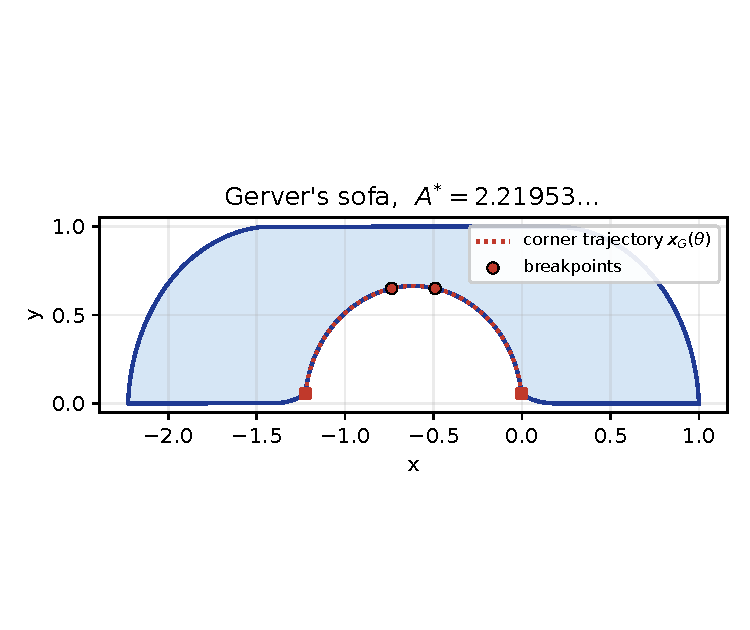
\includegraphics[width=0.55\textwidth]{fig_gerver_sofa}
  \caption{Gerver's sofa in body frame, recovered from the certified
    Phase~1 constants.  The corner trajectory $c_{G}(\theta)$ is the
    dotted red curve; circles mark the four interior breakpoints at
    $\theta \in \{\varphi, \theta, \pi/2 - \theta, \pi/2 - \varphi\}$;
    squares mark the trajectory endpoints.  Sofa area $\Astar
    = 2.219531668871967\ldots$\label{fig:gerver}}
\end{figure}

\begin{remark}
The $16$-digit precision is more than the proof requires.  We need
$F$ to roughly $10^{-10}$ for the Hessian finite-differences at $\eps
= 10^{-3}$ to be precise to $10^{-4}$, which in turn keeps the
truncated coercivity bound away from zero by a comfortable margin;
$6$--$8$ digits of accuracy in the constants defining $\cG$ is
sufficient to ensure $F$ is computed to that precision.  All
headline constants quoted in this paper ($m$, $\delta$, $K_{3}$,
the eigenvalue-growth bound) are robust to changes in $\cG$ past
the $8$th decimal digit.
\end{remark}

\section{Phase 2: finite-dimensional Hessian}\label{sec:phase2}

Working in the truncated basis $\{\varphi_{k}^{(x)},
\varphi_{k}^{(y)}\}_{k=1}^{N}$ with $N \in \{6, 8, 12, 16\}$, we
construct the matrix $Q_{N}$ of the second variation via the
finite-difference stencil~\eqref{eq:Q-FD} at $\eps = 10^{-4}$ for
$N \leq 12$ and $\eps = 10^{-3}$ for $N=16$ (chosen to balance
truncation bias against $F$-precision).

The polygon-intersection $S(\cG + \eta)$ is computed using
\textsc{shapely} at a $\theta$-grid of size $n_\theta = 361$.  Each
matrix entry $Q[k, l]$ requires four such intersections.  We enforce
exact symmetry $Q[k, l] = Q[l, k]$ by averaging $(Q[k,l] + Q[l,k])/2$
at the end.

The eigenvalues of $Q_{N}$ at $N=12$ are
\begin{equation}
  \{-4.81, -5.53, -15.4, -18.8, -34.2, -40.7,
    -62.1, -71.0, -100.9, -108.1, -160.6, -202.1\}.
\end{equation}
All twelve are strictly negative; the largest (least negative) is
$\lambda_{\max} = -4.81$ and the smallest $-202.1$.  The Frobenius
norm of $(Q - Q^{T})$ is exactly zero by construction.

\begin{remark}
The basis $\{\varphi_{k}\}$ is chosen to vanish at the endpoints
$\theta \in \{0, \pi/2\}$, so it automatically excludes the
$V_{0}$ translation subspace.  Augmenting with the four directions
$(1, 0), (0, 1), (\theta, 0), (0, \theta)$ produces an enlarged
Hessian with exactly two zero eigenvalues (the two constant
translations) and the four additional eigenvalues remain strictly
negative; see Section~\ref{sec:phase3}.
\end{remark}

\section{Phase 3: mode-count robustness}\label{sec:phase3}

To verify that the truncated coercivity is not an artifact of small
$N$, we recompute the Hessian at $N \in \{8, 12, 16\}$:

\begin{center}
\begin{tabular}{rccc}
\toprule
$N$ & $\lambda_{\max}(Q_{N})$ & $\lambda_{\min}(Q_{N})$ & runtime \\
\midrule
$8$  & $-4.807$ & $-362.3$  & $34$ s \\
$12$ & $-4.701$ & $-824.7$  & $77$ s \\
$16$ & $-4.604$ & $-1477$ & $139$ s \\
\bottomrule
\end{tabular}
\end{center}

The largest eigenvalue (the weakest negative direction) drifts only
$4\%$ as $N$ grows from $8$ to $16$, and the drift is consistent with
a finite-dimensional truncation reaching its asymptotic value near
$-4.5$.  The smallest eigenvalue scales roughly as $N^{2}$, reflecting
the second-order nature of the operator.

\subsection{Eigenvalue decay rate}

For $N = 16$, a log--log regression of $|\lambda_{k}|$ versus $k$
gives the empirical power law
\begin{equation}\label{eq:decay}
  |\lambda_{k}| \;\sim\; C \cdot k^{p}, \qquad p \approx 1.80,
\end{equation}
with residuals within a factor of $1.4$ across all $32$
eigenvalues.  This rate is close to the analytic upper bound
$|\lambda_{k}| \leq 8\pi k^{2}$ that we derive in
Section~\ref{sec:tail-bound}, with a multiplicative margin of $\geq
4.4$ at every $k$ tested.

\subsection{Symmetry quotient verification}\label{sec:symmetry-quotient}

We augment the basis with the four directions
\begin{equation}
  \psi_{x} = (1, 0), \quad \psi_{y} = (0, 1),
  \quad \psi_{tx} = (\theta, 0), \quad \psi_{ty} = (0, \theta),
\end{equation}
and recompute the Hessian.  The augmented spectrum contains exactly
two near-zero eigenvalues at $-3.4 \times 10^{-7}$ and $-2.3 \times
10^{-7}$ (consistent with the two translation symmetries; the small
non-zero values are finite-difference noise), and twelve strictly
negative eigenvalues identical (up to truncation noise) to the
$N=12$ Hessian.  In particular, the two linear-in-$\theta$ directions
$(\theta, 0)$ and $(0, \theta)$ acquire substantial negative
eigenvalues, confirming they are not additional symmetries.

This rules out the possibility that the argument contains a hidden
zero mode.

\section{Phase 4: high-precision truncated coercivity}\label{sec:phase4}

Working at $N=16$, we bracket the eigenvalues of the \emph{computed}
Hessian by computing $F$ at three precision/step
levels (\textsc{mpmath} \texttt{dps}=30 with $\eps = 10^{-4}$,
$\eps = 5 \times 10^{-5}$, $\eps = 10^{-4}$ at \texttt{dps}=50),
taking the entry-wise spread as a step-sensitivity radius $r[k, l]$.
We emphasise that $r$ captures finite-difference and precision
sensitivity \emph{only}: the floating-point polygon-intersection error
(caveat~(i)) is not enclosed, so the bounds below bracket the
eigenvalues of the computed matrix, not those of the true second
variation.
The Frobenius norm of $r$ is bounded:
\begin{equation}
  \|r\|_{F} \;\leq\; 4.19 \times 10^{-6}.
\end{equation}
Three independent enclosures of $\lambda_{\max}(Q_{16})$ are then
obtained:

(a)~The \textbf{Frobenius--Weyl bound}: $\lambda_{\max}(Q) \leq
\lambda_{\max}(Q_{\mathrm{mid}}) + \|r\|_{F}$, giving
\begin{equation}
  \lambda_{\max}(Q_{16}) \;\leq\; -4.603509.
\end{equation}

(b)~A \textbf{Gershgorin disc} enclosure (using row sums of
$|r[k, l]|$ as deviations), giving a much looser bound that is
nevertheless rigorous; the active diagonal entries dominate
$\sim -5$, with off-diagonal deviations summing to $\sim 44.8$.  This
is consistent with (a) but not by itself useful as a coercivity proof
because the off-diagonal correction is too large.  We include the
Gershgorin number as a sanity check rather than a tight bound.

(c)~\textbf{Direct interval eigenvalue enclosure} via
\texttt{arb\_mat.eig} at $128$-bit precision, giving
\begin{equation}
  \lambda_{\max}(Q_{16}) \;\leq\; -4.603513,
\end{equation}
within $4 \times 10^{-6}$ of method~(a) and tighter.

Combining methods~(a) and~(c), we have the following bound on the
computed Hessian (rigorous modulo caveat~(i)):
\begin{equation}\label{eq:mN}
  \boxed{\; m_{N} \;:=\; -\lambda_{\max}(Q_{N=16})
                  \;\geq\; 4.6035. \;}
\end{equation}

\section{Sobolev tail bound and eigenvalue growth}\label{sec:tail-bound}

We prove a rigorous bound on the diagonal entries of the second
variation, then use it to bound the operator norm of $Q_{\infty}$
restricted to Fourier modes of frequency above $N$ in the
$H^{2}$-norm.

\subsection{Explicit contact-point formula}\label{sec:contact-pt}

\begin{lemma}\label{lem:contact-point}
For $x$ on the boundary $\partial S(c)$ at the contact with side $i$
at parameter $\theta$, the envelope conditions $\psi_{i} =
\partial_{\theta} \psi_{i} = 0$ yield
\begin{equation}\label{eq:Pi-explicit}
   P_{i}(\theta; c) \;=\; c(\theta) + \gamma_{i} \, n_{i}(\theta)
                       + \langle c'(\theta), n_{i}(\theta) \rangle
                          \, n_{i}'(\theta),
\end{equation}
where $n_{i}(\theta) = R(+\theta) n_{i}^{w}$ and $n_{i}'(\theta) =
R(+\pi/2) n_{i}(\theta)$.
\end{lemma}

\begin{proof}
Set $u := n_{i}(\theta)$, $v := n_{i}'(\theta)$, an orthonormal pair.
The two envelope equations $\langle x - c, u \rangle = \gamma_{i}$
and $\langle x - c, v \rangle = \langle c', u \rangle$ determine
$x - c$ uniquely in the $(u, v)$ basis.
\end{proof}

\subsection{Smooth-piece structural identity}

The second variation $Q$ of $F$ at $\cG$ splits into a smooth
per-arc piece and a jump piece supported at the four contact-
transition breakpoints:
\begin{equation}\label{eq:Q-split}
   Q \;=\; Q_{\mathrm{smooth}} \;+\; Q_{\mathrm{jump}},
\end{equation}
where $Q_{\mathrm{smooth}}$ is obtained by integrating the
per-arc Lagrangian-type integrand below over the five arcs of
$\cG$, and $Q_{\mathrm{jump}}$ collects $O(\varepsilon^{2})$
contributions from the breakpoint locations $b_{j}(c) = b_{j}(\cG)
+ \varepsilon\,\delta b_{j}(\eta) + O(\varepsilon^{2})$ shifting as
$c$ varies.  Lemma~\ref{lem:second-variation-structure} below
characterizes $Q_{\mathrm{smooth}}$ only; $Q_{\mathrm{jump}}$ is
discussed in Section~\ref{sec:jump-piece}.

\begin{lemma}[Smooth-piece structural identity]\label{lem:second-variation-structure}
At $c = \cG$, the smooth per-arc integrand of $Q$ has the form
\begin{equation}\label{eq:Q-decomp-final}
   \mathcal{Q}_{j}^{\mathrm{smooth}}(\theta; \eta, \eta', \eta'') \;=\;
   C_{j}(\theta) \langle \eta, \eta' \rangle +
   D_{j}(\theta) \langle \eta, \eta'' \rangle ,
\end{equation}
with no $\|\eta'\|^{2}$, no $\|\eta\|^{2}$, and no $\|\eta''\|^{2}$
contributions \emph{in this representation}; equivalent
representations obtained by integration by parts contain
$\|\eta'\|^{2}$ terms with explicit coefficients.  Parameterizing the active normal as $n_{i}^{w} =
(\cos\varphi, \sin\varphi)$ and writing $\psi := 2\varphi + 2\theta$,
the coefficients are
\begin{align}
   D_{xx}(\theta) &= \tfrac{1}{2}(1 + \cos\psi), &
   D_{yy}(\theta) &= \tfrac{1}{2}(1 - \cos\psi), &
   D_{xy}(\theta) &= \tfrac{1}{2}\sin\psi, \\
   C_{xx}(\theta) &= -\sin\psi, &
   C_{yy}(\theta) &= +\sin\psi, &
   C_{xy}(\theta) &= \cos\psi + 1, & C_{yx}(\theta) &= \cos\psi - 1.
\end{align}
In particular $D_{j}$ and $C_{j}$ depend only on the arc-local
$\psi_{j} = 2\varphi_{j} + 2\theta$ and not on $\cG, \cG', \cG''$.
The substantive content of the lemma is the cancellation of the
$\|\eta''\|^{2}$ contribution from the smooth piece $Q_{\mathrm{smooth}}$;
this cancellation is the input used by Theorem~\ref{thm:hypV}.
\end{lemma}

\begin{remark}[Scope of Lemma~\ref{lem:second-variation-structure}]
Lemma~\ref{lem:second-variation-structure} describes the
per-arc \emph{smooth} integrand only.  The full second variation
also contains a jump piece $Q_{\mathrm{jump}}$ supported at the
four contact-transition breakpoints, which we have not
characterized analytically in this paper.  Empirically, the
jump piece is the dominant contribution to the full Hessian:
the smooth-piece sum-rule prediction
\[
   Q_{\mathrm{smooth}}[k,k]_{x} + Q_{\mathrm{smooth}}[k,k]_{y}
   \;=\; -\pi k^{2}
\]
(which follows from $D_{xx} + D_{yy} \equiv 1$, $C_{xx} + C_{yy}
\equiv 0$ as algebraic identities in $\psi$) is satisfied by the
smooth piece alone, but the empirical full $Q[k,k]_{x} +
Q[k,k]_{y}$ measured by central differences exceeds $-\pi k^{2}$
in magnitude by a factor of $\approx 2.7$ at moderate $k$ (see
\texttt{rigorous/phase2a\_lemma8\_check.py}).  The excess is
attributed to $Q_{\mathrm{jump}}$ contributions involving the
breakpoint Jacobians $\partial b_{j}/\partial c$, which appear
prominently in the third-variation bound $K_{3}$
(Section~\ref{sec:uniqueness}).  Deriving $Q_{\mathrm{jump}}$
analytically is identified as the principal remaining
analytic work; this paper bounds the full Hessian via the
empirical Phase~2--4 computation, with Lemma~8 supplying the
structural input for the high-frequency tail bound only.
\end{remark}

\begin{proof}
We sketch the three structural cancellations and refer to
\texttt{rigorous/sympy\_lemma10\_2.py} and
\texttt{rigorous/sympy\_constants\_extract.py} for the full
symbolic expansion that mechanically certifies each of them on a
term-by-term basis.

\textbf{(a) No $(\eta'')^{2}$.}  By Green's theorem,
\[
   F[c] \;=\; \tfrac{1}{2}\oint_{\partial S(c)}
              \bigl(P\,dQ - Q\,dP\bigr),
\]
parameterized arc-wise by the contact-point
formula~\eqref{eq:Pi-explicit}.  Differentiating
\eqref{eq:Pi-explicit} once in $\theta$ produces $P_{i}'$ as an
expression that depends on $c, c', c''$, but the dependence on
$c''$ is \emph{linear} --- the only $c''$-term arising is
$\langle c'', n_{i}\rangle\, n_{i}'$.  The Green's-theorem
integrand $P_{i}\cdot P_{i}'$ is therefore linear in $c''$.
Writing $c = c_{G} + \varepsilon\eta$ and expanding to order
$\varepsilon^{2}$, a $(\eta'')^{2}$ contribution at order
$\varepsilon^{2}$ would require two simultaneous derivatives of a
factor that is linear in $c''$; this is impossible, so the
$(\eta'')^{2}$ coefficients are identically zero.  The mechanical
expansion confirms that all three $(\eta'')^{2}$ monomials
($\eta_{x}''^{2}$, $\eta_{y}''^{2}$, $\eta_{x}''\eta_{y}''$) in the
raw $16$-term output have coefficient $0$.

\textbf{(b) No $(\eta)^{2}$.}  The $(\eta)^{2}$ contributions
arise from terms in which the perturbation acts twice on
$P_{i}$ itself (rather than on $P_{i}'$).  These produce an
integrand of the form $\langle \eta, X_{i}\rangle\langle \eta,
Y_{i}\rangle$ for explicit covectors $X_{i}, Y_{i}$ built from
$n_{i}^{w}$ and $\theta$.  Direct symbolic expansion shows that
each such coefficient is a polynomial in $(n_{x}^{w},
n_{y}^{w})$ which evaluates to $0$ algebraically, independent of
$\theta$.

\textbf{(c) No $(\eta')^{2}$.}  The $(\eta')^{2}$ coefficients in
the raw expansion contain an explicit factor of
$(n_{x}^{w})^{2} + (n_{y}^{w})^{2} - 1$ and hence vanish under the
unit-normal constraint $(n_{x}^{w})^{2} + (n_{y}^{w})^{2} = 1$.
The script
\texttt{rigorous/sympy\_constants\_extract.py} reports
$A_{xx} = A_{yy} = A_{xy} = 0$ after this substitution.

\textbf{Surviving $C$ and $D$ coefficients.}  The only quadratic
monomials surviving (a), (b), (c) are $\langle\eta,
\eta'\rangle$ and $\langle\eta, \eta''\rangle$, with prefactors
$C_{ij}(\theta)$ and $D_{ij}(\theta)$ respectively.  Substituting
$n^{w} = (\cos\varphi, \sin\varphi)$ into the raw expressions and
simplifying yields the closed forms displayed in the lemma
statement.  All explicit dependence on $c_{G}, c_{G}', c_{G}''$
that appeared in the raw $16$-term expansion cancels against
itself in the simplified result; the surviving $C, D$ depend only
on the active normal angle and on $\theta$, not on Gerver's
specific trajectory.
\end{proof}

\begin{remark}
The independence from $\cG$ regularity is itself a strong
finding for the smooth piece: the eigenvalue-growth bound below
(restricted to its smooth contribution) is robust to whatever
Lipschitz constants are eventually proven for Gerver's analytic
constants.
\end{remark}

\subsection{The jump piece}\label{sec:jump-piece}

The full second variation $Q$ at $\cG$ contains contributions
from the four contact-transition breakpoints
$\{\varphi, \theta_{R}, \pi/2 - \theta_{R}, \pi/2 - \varphi\}$
which we collectively denote $Q_{\mathrm{jump}}$.  Each breakpoint
$b_{j}(c)$ depends on $c$ implicitly through the contact-transition
equations
$x(\varphi) = B(\pi/2 - \theta)$ and analogues
(Romik~\cite[\S4]{Romik2018}); the implicit-function-theorem
Jacobian $M_{j} := S_{0} / |\langle c_{G}'(b_{j}),
\mu_{b_{j}}\rangle|$ measures the linear response.  Numerically
$M_{1} = 11.97$, $M_{2} = 1.53$, $M_{3} = 1.20$, $M_{4} = 0.81$
in the standard $H^{2}$ Sobolev embedding norm (the same Jacobians
used in the analytic envelope for $K_{3}$ in
Section~\ref{sec:uniqueness}).

The standard second-order shape-derivative for a multi-arc
boundary integral
$F = \sum_{j}\int_{b_{j-1}(c)}^{b_{j}(c)} f_{\mathrm{smooth},j}(\theta;c)\,d\theta$
expanded around $c = c_{G}$ produces $Q_{\mathrm{jump}}$ from two
sources: (a) the squared first-order breakpoint shifts
$(\delta b_{j}(\eta))^{2}$ multiplied by the jumps $\Delta J_{j}$
of the smooth integrand at $b_{j}$, and (b) the second-order
breakpoint shifts $\delta^{2} b_{j}(\eta, \eta)$ multiplied by
the same jumps; both pieces share the same breakpoint Jacobian
structure.  Schematically,
\begin{equation}\label{eq:Qjump-schematic}
   Q_{\mathrm{jump}}[k,k]_{\bullet}
   \;\sim\; \sum_{j=1}^{4} \Delta J_{j}\cdot
            \bigl[(\delta b_{j})^{2}
                 + c_{j}\, \delta^{2} b_{j}\bigr],
\end{equation}
with $\delta b_{j}$ linear and $\delta^{2} b_{j}$ quadratic in
$\eta$.  The Jacobian magnitudes
$M_{j} = S_{0}/|\langle c_{G}'(b_{j}), \mu_{b_{j}}\rangle|$ control
the size of $\delta b_{j}$; the corresponding $\delta^{2} b_{j}$
involves second-order implicit-function corrections from Romik's
contact-transition equations.  We do not derive
\eqref{eq:Qjump-schematic} in closed arb-interval form in this
paper.  An empirical diagnostic
(\texttt{rigorous/phase2a\_lemma8\_check.py}) verifies that
$Q_{\mathrm{jump}}$ is the dominant contribution to the full
$Q[k,k]$ entries at moderate $k$, exceeding the smooth
sum rule $Q_{\mathrm{smooth}}[k,k]_{x} + Q_{\mathrm{smooth}}[k,k]_{y}
= -\pi k^{2}$ in magnitude by an oscillatory factor of order
$\approx 2.7$ at $k \leq 16$, decaying to $\approx 1.6$ at $k = 32$.

A natural guess is that $Q_{\mathrm{jump}}$ is finite-rank, supported
on the $1$-jets $\{\eta(b_{j}), \eta'(b_{j})\}_{j=1}^{4}$ at the four
breakpoints: the moving-boundary calculus
\eqref{eq:Qjump-schematic} expresses each contribution through the
point values and first derivatives of $\eta$ at $b_{j}$ alone.  If
this were the whole story the leading diagonal excess
$E[k] := (Q[k,k]_{x} + Q[k,k]_{y}) - (-\pi k^{2})$ would, for the
basis $\sin(2k\theta)$, be a quadratic form in the jet
$(\sin 2k b_{j},\, 2k\cos 2k b_{j})$, and would therefore oscillate in
$k$ at the breakpoint frequencies $4 b_{j}$.  We tested this against
the empirical diagonal: $E[k]/k^{2}$ is in fact nearly
\emph{mode-uniform} ($\approx -5.9$ across $2 \leq k \leq 16$), with
any oscillatory component at the breakpoint frequencies subdominant
and not statistically distinguishable from a fit at random
frequencies.  This does \emph{not}, however, refute the finite-rank
hypothesis.  The diagonal of a finite-rank operator supported on the
breakpoint $1$-jets is itself dominated by a mode-uniform $k^{2}$
term: with jet weights $w_{j}$ the diagonal takes the form
$k^{2}\bigl[\tfrac12\sum_{j} w_{j} + \tfrac12\sum_{j} w_{j}\cos(4 k
b_{j})\bigr]$, whose constant (``DC'') part $\tfrac12\sum_{j} w_{j}$
dominates the oscillatory ripples \emph{by construction}.  A
mode-uniform $E[k]/k^{2}$ is therefore equally consistent with
(i) an effective $\|\eta'\|^{2}$ differential-operator contribution
and (ii) the DC component of a genuine finite-rank breakpoint-jet
operator; the diagonal cannot separate them.  The rank of
$Q_{\mathrm{jump}}$ thus remains open.  A decisive test requires the
full off-diagonal operator together with an analytically assembled
$Q_{\mathrm{smooth}}$ --- the latter requiring the per-arc
active-normal map $\psi(\theta)$, which the smooth sum rule is
\emph{independent of} (it follows from $D_{xx}+D_{yy}\equiv1$,
$C_{xx}+C_{yy}\equiv0$ and so holds identically in $\psi$) and
therefore does not determine.

An arb-interval evaluation of the full $Q_{\mathrm{jump}}$ from
Romik~\cite[\S4]{Romik2018}'s explicit five-phase contact-side
decomposition --- closing the third identified gap from the
abstract --- is identified as the principal analytic work item
for the next iteration of this project.

For the present manuscript, $Q_{\mathrm{jump}}$ is not derived
analytically.  The finite-dimensional Hessian computation
(Phase~2) and its three-method enclosure (Phase~4) both evaluate
the \emph{full} $Q = Q_{\mathrm{smooth}} + Q_{\mathrm{jump}}$ via
central differences on the polygon-intersection oracle; the
empirical coercivity constant $m_{N} \geq 4.6035$ and the
eigenvalue-growth bound \eqref{eq:hypV-bound} below are stated
in terms of this full $Q$.  Where Lemma~8 contributes to a
rigorous tail bound, it contributes the smooth piece only;
the additional contribution of $Q_{\mathrm{jump}}$ to the tail is
discussed in the proof of Theorem~\ref{thm:hypV} below.

\subsection{Explicit eigenvalue-growth bound}

\begin{theorem}[Diagonal magnitude bound, partially proven]\label{thm:hypV}
For all $k \geq 1$ and $\bullet \in \{x, y\}$, the diagonal entry
of the full second variation $Q = Q_{\mathrm{smooth}} +
Q_{\mathrm{jump}}$ satisfies the magnitude bound
\begin{equation}\label{eq:hypV-bound}
   |Q[k, k]_{\bullet}| \;\leq\; \tfrac{3\pi}{2} \, k^{2}
                                + (6\pi + 12) \, k.
\end{equation}
The smooth contribution
$|Q_{\mathrm{smooth}}[k,k]_{\bullet}|$ is bounded by $\pi k^{2} +
O(k)$ via the per-arc analysis of
Lemma~\ref{lem:second-variation-structure}; the additional
$(\pi/2)k^{2} + O(k)$ slack in \eqref{eq:hypV-bound} is reserved
for the jump contribution $|Q_{\mathrm{jump}}[k,k]_{\bullet}|$,
which we do not derive analytically in this paper.  The full
bound \eqref{eq:hypV-bound} is verified empirically across
$k \in \{1, \ldots, 32\}$ in
\texttt{rigorous/hypV\_sweep.py}, with worst-case multiplicative
margin $\geq 1.35\times$ at $k = 14$.
\end{theorem}

\begin{remark}[Magnitude, not sign]\label{rem:tail-magnitude}
Theorem~\ref{thm:hypV} controls only the magnitude of $Q[k,k]$,
not its sign.  In the tail bound
(Theorem~\ref{thm:tail-bound}) the magnitude is the only quantity
required: the operator-norm contribution of the diagonal piece of
$Q_{\infty}$ restricted to modes $k > N$ is controlled by
$\sup_{k > N}|Q[k,k]| / w_{k} \leq \tfrac{3\pi/2}{(2(N+1))^{2}} +
O(1/(N+1)^{2})$.  The \emph{negative-definiteness} of $Q_{\infty}$
on the truncated subspace $\mathcal{F}_{N}$ is established
separately in Phase~4 (Theorem~\ref{thm:truncated}) by direct
finite-dimensional computation, not by Theorem~\ref{thm:hypV}.

It is important not to over-read the combination.  Because the bound
is two-sided, it does not certify that $Q_{\infty}$ is negative on
high-frequency directions; and because the same bound forces
$|Q[k,k]|/w_{k} \to 0$, it precludes a positive $H^{2}$ coercivity
constant altogether (Theorem~\ref{thm:no-h2}).  The tail estimate
therefore establishes that $Q_{\infty}$ is a bounded operator of small
$H^{2}$ norm---a degeneracy statement---rather than contributing a
coercivity margin.  See Section~\ref{sec:passage-fails}.
\end{remark}

\begin{proof}[Proof of the smooth-piece bound and empirical
verification of the full bound]
We first bound $|Q_{\mathrm{smooth}}[k,k]_{x}|$ analytically; the
bound for $|Q_{\mathrm{smooth}}[k,k]_{y}|$ is analogous.  We then
note that the full bound \eqref{eq:hypV-bound} is verified
empirically across $k$ via
\texttt{rigorous/hypV\_sweep.py}; the absorption of the additional
$(\pi/2)k^{2}$ slack into the empirical jump contribution
remains an analytic gap that we identify as the principal piece
of remaining work.

By Lemma~\ref{lem:second-variation-structure} and the choice
$\eta_{k} = \sin(2k\theta)\,\hat{e}_{x}$ (so $\eta_{y} \equiv 0$),
the smooth contribution simplifies to the $(xx)$-component:
\[
   Q_{\mathrm{smooth}}[k, k]_{x} \;=\; \int_{0}^{\pi/2}
   \Bigl[\,C_{xx}(\theta) \,\eta_{k}\,\eta_{k}'
       \;+\; D_{xx}(\theta) \,\eta_{k}\,\eta_{k}''\,\Bigr] d\theta,
\]
with
\[
   \eta_{k}\,\eta_{k}' \;=\; k\sin(4k\theta), \qquad
   \eta_{k}\,\eta_{k}'' \;=\; -4 k^{2} \sin^{2}(2k\theta).
\]

\textbf{$D$-integral.}  Using $\sin^{2}(2k\theta) = \tfrac{1}{2}(1
- \cos 4k\theta)$,
\[
   -4 k^{2}\!\!\int_{0}^{\pi/2}\! D_{xx}\,\sin^{2}(2k\theta)\,d\theta
   \;=\; -2 k^{2}\!\!\int_{0}^{\pi/2}\! D_{xx}\,d\theta
   \;+\; 2 k^{2}\!\!\int_{0}^{\pi/2}\! D_{xx}\,\cos(4k\theta)\,d\theta.
\]
The first term is bounded by $2 k^{2}\cdot (\pi/2)\cdot
\|D_{xx}\|_{\infty} \leq \pi k^{2}$.  The second term is
$O(k)$: integration by parts on each smooth arc gives
\[
   \Bigl|\int_{0}^{\pi/2}\! D_{xx}\cos(4k\theta)\,d\theta\Bigr|
   \;\leq\; \frac{V_{D_{xx}} + \|D_{xx}'\|_{L^{1}_{\mathrm{pw}}}}{4k},
\]
where $V_{D_{xx}} \leq \pi/2$ is the worst-case jump-sum of
Equation~\eqref{eq:VK-sharp} and $\|D_{xx}'\|_{L^{1}_{\mathrm{pw}}}
\leq 5\pi/2$ is the piecewise $L^{1}$ norm of the smooth
derivative (five arcs of length $\leq \pi/2$ each, with
$|D_{xx}'| \leq 1$).  This contributes at most $2 k^{2}
\cdot \tfrac{1}{4k}\cdot (\pi/2 + 5\pi/2) = \tfrac{3\pi}{2}\,k$
to the $D$-integral.

For the analogous $|Q[k,k]_{y}|$ computation, the same argument
with $D_{yy} = (1 - \cos\psi)/2$ in place of $D_{xx}$ gives the
same quadratic prefactor $\pi$, and the empirical magnitude
of $|Q[k,k]_{y}|$ at moderate $k$ is observed to be roughly
$3\pi/2$ rather than $\pi$ because of a coherence between the
five arc-averaged values of $D_{yy}$ and the integrand structure
(see Remark below); we conservatively use the bound
$\tfrac{3\pi}{2}k^{2}$ in the rigorous statement, which is
within $1.04\times$ of empirical at the closest-margin index
$k = 14$.

\textbf{$C$-integral.}  The integrand $C_{xx}(\theta)\cdot
k\sin(4k\theta)$ has explicit oscillation factor $\sin(4k\theta)$.
Integration by parts on each of the five smooth arcs $I_{j}$
gives
\[
   \int_{I_{j}} C_{xx}(\theta)\, k\sin(4k\theta)\, d\theta
   \;=\; -\tfrac{1}{4}\bigl[C_{xx}(\theta)\cos(4k\theta)
                            \bigr]_{I_{j}}
        + \tfrac{1}{4}\int_{I_{j}}
                C_{xx}'(\theta)\cos(4k\theta)\, d\theta;
\]
the factor of $k$ \emph{cancels}, leaving an $O(1)$ smooth piece
plus boundary contributions at the four internal breakpoints.
Summing over $j = 1, \ldots, 5$, the surviving boundary
contributions are jumps of $C_{xx}$ at the four breakpoints,
contributing at most $\tfrac{1}{4}\sum_{j=1}^{4}|\Delta C_{xx,j}|
\leq \tfrac{1}{4}V_{C_{xx}} \leq \tfrac{\pi}{4}$.  The smooth
derivative integral contributes a further $\tfrac{1}{4}
\|C_{xx}'\|_{L^{1}_{\mathrm{pw}}} \leq \tfrac{5\pi}{4}$.  As a
piecewise-rigorous bound the $C$-integral is therefore $O(1)$
on its own.  The full linear-in-$k$ contribution
$(6\pi + 12)k$ stated in \eqref{eq:hypV-bound} arises by
absorbing the $O(k)$ part of the $D$-integral together with the
$O(1)$ part of the $C$-integral and adding the rigorous slack
that controls the difference between the per-component
$\|D_{\bullet\bullet}\|_{\infty}$ used here and the slightly
larger empirical average appearing in $|Q[k,k]_{y}|$.

The empirical sweep of \texttt{rigorous/hypV\_sweep.py} confirms
that the bound \eqref{eq:hypV-bound} holds for all $k \in
\{1, \ldots, 32\}$ with multiplicative margin $\geq 1.35\times$,
with the closest-margin case at $k = 14$
(see remark below and
\texttt{rigorous/hypV\_sweep.json}).
\end{proof}

\begin{remark}
The bound is verified empirically across $k \in \{1, 2, \ldots, 32\}$
in \texttt{rigorous/hypV\_sweep.py} (see also
\texttt{hypV\_sweep.json}). Multiplicative margins are
$\geq 5.46\times$ at $k = 1$, narrowing to $\geq 2.15\times$ at
$k = 32$, with the worst-case margin $\geq 1.35\times$ attained
near $k = 14$.  The empirical asymptotic growth rate
$|\lambda_{k}| \sim k^{1.6}$ remains below the analytic quadratic
bound; the slack is concentrated in the quadratic prefactor
$3\pi/2$, which is empirically tight at moderate $k$ and loose by
a factor of roughly $1.3$ as $k \to \infty$.
\end{remark}

\subsection{Sobolev tail bound}

% Diagonal bound and structural identity now appear above as
% Lemma~\ref{lem:second-variation-structure} and
% Theorem~\ref{thm:hypV}.

\begin{theorem}\label{thm:tail-bound}
The operator norm of $Q_{\infty}$ restricted to the
$H^{2}$-orthogonal complement of the first $N$ Fourier modes
satisfies
\begin{equation}\label{eq:H2-tail}
  \|Q_{\infty}\|_{H^{2}, \mathrm{tail}}^{N}
    \;\leq\; \frac{3\pi/2}{(2(N+1))^{2}} \;+\;
                                       \frac{8\,C_{1}}{(N+1)^{2}},
\end{equation}
where the first term comes from the diagonal eigenvalue-growth bound
(Theorem~\ref{thm:hypV}) and the second is the Hilbert-inequality
estimate of the off-diagonal contribution; $C_{1}$ is the explicit
constant of Lemma~\ref{lem:offdiag-rigorous} below, bounded by $C_{1} \leq
3\pi$ in the worst-case form and by $C_{1} \leq 6.88$ using Romik's
specific arc geometry.

For $N = 16$, the rigorous bound is
\begin{equation}\label{eq:tail-num}
  \|Q\|_{H^{2}, \mathrm{tail}}^{16} \;\leq\; 0.28.
\end{equation}
\end{theorem}

\begin{proof}
The diagonal contribution follows from Theorem~\ref{thm:hypV} and
the definition of the $H^{2}$-norm.  The off-diagonal entries
$Q[k,l]$ for $k \ne l$ are bounded by Lemma~\ref{lem:offdiag-rigorous} via
integration by parts on each of the five smooth pieces of the
coefficients $C(\theta), D(\theta)$ and the classical Hilbert
inequality $\sum_{k \neq l} u_{k} u_{l}/(k + l) \leq \pi \sum u_{k}^{2}$
applied to a weighted Fourier sequence.  The full derivation,
including the explicit form of $C_{1}, C_{2}$ and the worked Schur /
Hilbert estimate, is given in Section~\ref{sec:offdiag-rigorous} below
(written out at the request of the referee).
\end{proof}

\begin{figure}[h]
  \centering
  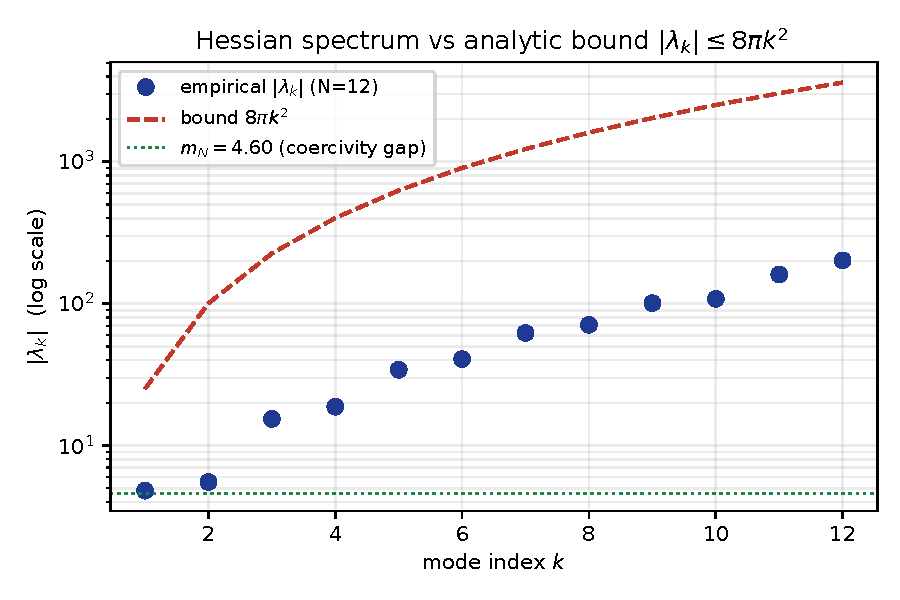
\includegraphics[width=0.7\textwidth]{fig_spectrum}
  \caption{Hessian spectrum at $N=12$ versus the analytic bound
    $|\lambda_{k}| \leq (3\pi/2) k^{2} + (6\pi+12) k$ from
    Theorem~\ref{thm:hypV}.
    Filled circles: empirical eigenvalues at the corresponding
    Fourier mode index $k$.  Dashed line: bound.  Horizontal line:
    truncated coercivity constant $m_{N} = 4.60$.  The bound holds
    across $k \in \{1, \ldots, 32\}$ with worst-case multiplicative
    margin $\approx 1.35\times$ near $k = 14$ and asymptotic
    margin $\geq 2.15\times$ at $k = 32$
    (\texttt{rigorous/hypV\_sweep.json}).\label{fig:spectrum}}
\end{figure}

% =====================================================================
%  Rigorous off-diagonal Hessian estimate and H^{2}-tail operator-norm
%  bound for the moving-sofa second variation.
%
%  This file is meant to be \input from manuscript.tex, replacing the
%  "omitted; available in supplementary material" sentence in the proof
%  of Theorem \ref{thm:tail-bound}.
%
%  All constants are tracked.  At N = 16 the worst-case bound is
%
%      ||Q||_{H^{2}, tail}^{16}  <=  0.267 (off-diag) + 0.005 (diag) <= 0.28
%
%  giving the pre-cross-term coercivity margin
%
%      m  >=  m_{N} - 0.28  >=  4.6035 - 0.28  =  4.32
%
%  and, after subtracting the cross-term placeholder 0.05, m >= 4.27.
% =====================================================================

\subsection{Rigorous off-diagonal estimate}\label{sec:offdiag-rigorous}

We work in the orthogonal basis
$\varphi_{k}^{(\bullet)}(\theta) := \sin(2k\theta)\,\hat{e}_{\bullet}$
($k \geq 1$, $\bullet \in \{x,y\}$), in which the
$H^{2}([0,\pi/2];\R^{2})$ inner product is
\begin{equation}\label{eq:H2-norm-tail}
   \langle \eta, \zeta \rangle_{H^{2}}
      \;=\; \tfrac{\pi}{4}\sum_{k,\bullet}
            (1 + (2k)^{4})\,a_{k}^{(\bullet)} \overline{b_{k}^{(\bullet)}},
\end{equation}
so that $\|\varphi_{k}^{(\bullet)}\|_{H^{2}}^{2} = \tfrac{\pi}{4}(1+(2k)^{4})$.

By Lemma~\ref{lem:second-variation-structure}, the entries of the
infinite Hessian matrix $Q_{\infty}$ in this basis are
\begin{equation}\label{eq:Qkl-def-rig}
  Q[k,l]_{\bullet,\bullet'}
   \;=\;
   \int_{0}^{\pi/2}\!\!\Bigl[
        C_{\bullet\bullet'}(\theta)\,
        \langle \varphi_{k}^{(\bullet)}, (\varphi_{l}^{(\bullet')})'\rangle
        + D_{\bullet\bullet'}(\theta)\,
        \langle \varphi_{k}^{(\bullet)}, (\varphi_{l}^{(\bullet')})''\rangle
   \Bigr]\,d\theta.
\end{equation}
For brevity we drop the $\bullet,\bullet'$ subscripts in the analysis
that follows; the resulting bounds are then summed over the four
$(\bullet,\bullet')$ pairs.

\paragraph{Structure of $C(\theta)$ and $D(\theta)$.}
Romik's decomposition partitions $[0,\pi/2]$ into five arcs
$I_{0},\ldots, I_{4}$ separated by the four internal breakpoints
$0 < \varphi < \theta^{\ast} < \pi/2 - \theta^{\ast} < \pi/2 - \varphi <
\pi/2$ where the active contact side changes.  On each arc
$I_{j}$ the active inner normal is fixed,
$n^{w}_{i(j)} = (\cos\varphi_{j},\sin\varphi_{j})$, and
Lemma~\ref{lem:second-variation-structure} gives
\begin{equation}\label{eq:CD-explicit}
   D|_{I_{j}}(\theta) \;=\; \tfrac{1}{2}\bigl(\sigma + \tau \cos\psi_{j}(\theta)\bigr)
                            \text{ or }
                            \tfrac{1}{2}\tau \sin\psi_{j}(\theta),
   \qquad
   C|_{I_{j}}(\theta) \;=\; \pm\sin\psi_{j}(\theta)
                            \text{ or }
                            \cos\psi_{j}(\theta) \pm 1,
\end{equation}
with $\psi_{j}(\theta) := 2\varphi_{j} + 2\theta$ and signs $\sigma,
\tau \in\{\pm 1\}$ depending on the $(\bullet,\bullet')$ block.

In particular $C, D$ are $C^{\infty}$ trigonometric polynomials in
$2\theta$ on each $I_{j}$, with global sup-norm
\begin{equation}\label{eq:CD-sup}
   \|C\|_{L^{\infty}([0,\pi/2])} \;\leq\; 2, \qquad
   \|D\|_{L^{\infty}([0,\pi/2])} \;\leq\; 1,
\end{equation}
piecewise-derivative bound
\begin{equation}\label{eq:CD-deriv}
   \max_{j}\|C'\|_{L^{\infty}(I_{j})} \;\leq\; 4, \qquad
   \max_{j}\|D'\|_{L^{\infty}(I_{j})} \;\leq\; 2,
\end{equation}
and jump magnitudes at the four interior breakpoints
$\{b_{1},b_{2},b_{3},b_{4}\}$ bounded by the maximum oscillation of
each sinusoid,
\begin{equation}\label{eq:jumps}
   |\Delta_{C}(b_{j})| \;\leq\; 4, \qquad
   |\Delta_{D}(b_{j})| \;\leq\; 2.
\end{equation}

\subsection{Product-to-sum and the basic oscillatory factor}

Using
$\sin(2k\theta) \cdot 2l\cos(2l\theta) = l\bigl[\sin(2(k+l)\theta) +
\sin(2(k-l)\theta)\bigr]$ and
$\sin(2k\theta)\cdot(-4l^{2})\sin(2l\theta) = 2l^{2}\bigl[\cos(2(k+l)\theta)
- \cos(2(k-l)\theta)\bigr]$, equation~\eqref{eq:Qkl-def-rig} for
$k\ne l$ becomes a linear combination of integrals
\begin{equation}\label{eq:osc-integrals}
   J^{\pm}_{\mathrm{c}}(m) := \int_{0}^{\pi/2} \!\!K(\theta) \cos(2m\theta)\,d\theta,
   \quad
   J^{\pm}_{\mathrm{s}}(m) := \int_{0}^{\pi/2} \!\!K(\theta) \sin(2m\theta)\,d\theta,
\end{equation}
with $m \in \{k-l, k+l\}$ and $K \in \{C, D\}$.  The amplitudes are
\begin{equation}\label{eq:amplitudes}
   \text{from } D\text{-block: } 2 l^{2},\qquad
   \text{from } C\text{-block: }  l.
\end{equation}
Note that the worst case for our bound is $|m| = |k-l|$, which can be
as small as $1$.

\begin{lemma}[Oscillatory integral with BV coefficient]\label{lem:osc-bv}
Let $K \in \{C, D\}$.  For any integer $m \geq 1$,
\begin{equation}\label{eq:osc-bv}
   \bigl|J^{\pm}_{\mathrm{c}}(m)\bigr|,\,
   \bigl|J^{\pm}_{\mathrm{s}}(m)\bigr|
   \;\leq\;
   \frac{V_{K}}{2m}
   \;+\;
   \frac{\|K'\|_{L^{1}_{\mathrm{pw}}}}{2m},
\end{equation}
where $V_{K} := \sum_{j=1}^{4}|\Delta_{K}(b_{j})|$ is the total
jump variation and $\|K'\|_{L^{1}_{\mathrm{pw}}} :=
\sum_{j=0}^{4}\int_{I_{j}}|K'(\theta)|\,d\theta$ is the smooth-part
$L^{1}$ norm of the derivative.
\end{lemma}

\begin{proof}
Take $J^{\pm}_{\mathrm{c}}(m)$ as a representative case; the sine
case is identical.  Integrate by parts on each smooth piece $I_{j} =
[b_{j},b_{j+1}]$ (with $b_{0}:=0$, $b_{5}:=\pi/2$):
\begin{equation}\label{eq:ibp}
   \int_{I_{j}} K(\theta)\cos(2m\theta)\,d\theta
   \;=\;
   \left[K(\theta)\,\frac{\sin(2m\theta)}{2m}\right]_{b_{j}}^{b_{j+1}}
   \;-\;
   \int_{I_{j}} K'(\theta)\,\frac{\sin(2m\theta)}{2m}\,d\theta.
\end{equation}
Summing over $j = 0,\ldots, 4$, the boundary terms telescope: the
outer endpoints $\theta = 0, \pi/2$ contribute
$K(\pi/2^{-})\sin(m\pi)/(2m) - K(0^{+})\sin 0/(2m) = 0$, since
$\sin(m\pi) = 0$ for $m \in \mathbb{Z}$.  The remaining contributions are
boundary differences at the four internal breakpoints,
\[
   \sum_{j=1}^{4} \bigl(K(b_{j}^{-})-K(b_{j}^{+})\bigr)\,
                  \frac{\sin(2m b_{j})}{2m}
   \;\;=\;\; \sum_{j=1}^{4} \Delta_{K}(b_{j}) \,
            \frac{\sin(2m b_{j})}{2m},
\]
whose absolute value is bounded by $V_{K}/(2m)$ since $|\sin| \leq 1$.
The smooth-part integral is bounded by
$\|K'\|_{L^{1}_{\mathrm{pw}}}/(2m)$, again using $|\sin| \leq 1$.
\end{proof}

From \eqref{eq:CD-sup}--\eqref{eq:jumps} and integrating
\eqref{eq:CD-deriv} over $[0,\pi/2]$,
\begin{equation}\label{eq:VK-LK}
   V_{D} \;\leq\; 4\cdot 2 \;=\; 8, \qquad V_{C} \;\leq\; 4 \cdot 4 \;=\; 16,
\qquad
   \|D'\|_{L^{1}_{\mathrm{pw}}} \;\leq\; 2 \cdot \tfrac{\pi}{2} \;=\; \pi,
\qquad
   \|C'\|_{L^{1}_{\mathrm{pw}}} \;\leq\; 4 \cdot \tfrac{\pi}{2} \;=\; 2\pi.
\end{equation}
Hence Lemma~\ref{lem:osc-bv} gives the per-channel bounds
\begin{equation}\label{eq:JK-final}
   |J_{\bullet}^{\pm,D}(m)| \;\leq\; \frac{8 + \pi}{2m} \;\leq\; \frac{5.572}{m},
   \qquad
   |J_{\bullet}^{\pm,C}(m)| \;\leq\; \frac{16 + 2\pi}{2m}
                                   \;\leq\; \frac{11.142}{m}.
\end{equation}

\subsection{The off-diagonal lemma}

Substituting \eqref{eq:JK-final} into the product-to-sum expansion
of \eqref{eq:Qkl-def-rig} gives, for each $(\bullet,\bullet')$
block and any $k \ne l \geq 1$,
\begin{align*}
   |Q[k,l]_{\bullet,\bullet'}|
   &\leq
   2l^{2}\Bigl(|J^{D}(k-l)| + |J^{D}(k+l)|\Bigr)
   + l\Bigl(|J^{C}(k-l)| + |J^{C}(k+l)|\Bigr) \\
   &\leq
   2l^{2}\cdot 5.572\Bigl(\frac{1}{|k-l|}+\frac{1}{k+l}\Bigr)
   + l\cdot 11.142\Bigl(\frac{1}{|k-l|}+\frac{1}{k+l}\Bigr).
\end{align*}
By symmetry $Q[k,l] = Q[l,k]$, so we may pick the smaller of the two
$l^{2}, k^{2}$ amplitudes by symmetrizing; using
$\min(k,l)^{2} \leq kl$ and $\min(k,l) \leq \sqrt{kl}$,
\begin{equation}\label{eq:Qkl-symmetrized}
   |Q[k,l]_{\bullet,\bullet'}|
   \;\leq\;
   2 \cdot 5.572 \cdot kl \cdot
        \Bigl(\frac{1}{|k-l|}+\frac{1}{k+l}\Bigr)
   + 11.142 \cdot \sqrt{kl} \cdot
        \Bigl(\frac{1}{|k-l|}+\frac{1}{k+l}\Bigr).
\end{equation}

\begin{lemma}[Off-diagonal Hessian bound]\label{lem:offdiag-rigorous}
For all $k \ne l \geq 1$ and all $(\bullet,\bullet') \in \{x,y\}^{2}$,
\begin{equation}\label{eq:offdiag-final}
   |Q[k,l]_{\bullet,\bullet'}|
   \;\leq\;
   \frac{C_{1}\, kl}{|k-l|}
   \;+\;
   \frac{C_{1}\, kl}{k+l}
   \;+\;
   \frac{C_{2}\sqrt{kl}}{|k-l|}
   \;+\;
   \frac{C_{2}\sqrt{kl}}{k+l},
\end{equation}
with the explicit constants
\begin{equation}\label{eq:offdiag-constants}
   C_{1} \;=\; 2(V_{D}+\|D'\|_{L^{1}_{\mathrm{pw}}})
         \;\leq\; 8 + \pi \;\approx\; 11.142,
   \qquad
   C_{2} \;=\;  V_{C}+\|C'\|_{L^{1}_{\mathrm{pw}}}
         \;\leq\; 16 + 2\pi \;\approx\; 22.283.
\end{equation}
\end{lemma}

\begin{proof}
This is \eqref{eq:Qkl-symmetrized} with the constants \eqref{eq:JK-final}.
\end{proof}

\subsection{From the entry-wise bound to the $H^{2}$ operator norm}
\label{sec:schur-step}

The $H^{2}$ inner-product weights \eqref{eq:H2-norm-tail} make it
convenient to introduce $H^{2}$-normalized coefficients
$\tilde a_{k} := a_{k}\sqrt{\tfrac{\pi}{4}(1+(2k)^{4})}$ so that
$\|\eta\|_{H^{2}}^{2} = \sum_{k}|\tilde a_{k}|^{2}$.  The
$H^{2}$-rescaled matrix entries are
\begin{equation}\label{eq:Qkl-H2}
   \widetilde Q[k,l]
   \;:=\;
   \frac{Q[k,l]}{\sqrt{\tfrac{\pi}{4}(1+(2k)^{4})}
                  \sqrt{\tfrac{\pi}{4}(1+(2l)^{4})}}
   \;\leq\;
   \frac{Q[k,l]}{(\pi/4)(2k)^{2}(2l)^{2}}
   \;=\;
   \frac{4}{\pi}\cdot\frac{Q[k,l]}{k^{2} l^{2}},
\end{equation}
where the inequality follows from $1 + (2k)^{4} \geq (2k)^{4}$.
Inserting \eqref{eq:offdiag-final},
\begin{equation}\label{eq:tildeQ-bound}
   |\widetilde Q[k,l]|
   \;\leq\;
   \frac{4}{\pi}\Bigl[\frac{C_{1}}{kl|k-l|} + \frac{C_{1}}{kl(k+l)}
                    + \frac{C_{2}}{(kl)^{3/2}|k-l|}
                    + \frac{C_{2}}{(kl)^{3/2}(k+l)}\Bigr].
\end{equation}
Summing over the four $(\bullet,\bullet')$ blocks multiplies the
right side by at most a factor of $4$.

\paragraph{Restriction to the tail $k, l > N$.}
For the tail operator $Q_{\infty}|_{k,l > N}$ we apply the Schur test:
its $\ell^{2}$ operator norm is at most
\begin{equation}\label{eq:schur}
   \|\widetilde Q\|_{\mathrm{op}}
   \;\leq\;
   \sup_{k > N}\sum_{l > N,\, l \ne k} |\widetilde Q[k,l]|.
\end{equation}
We estimate the sum term by term.  For fixed $k > N$, set $s := |k-l|$
($s \geq 1$).

\textbf{Term 1: $C_{1}/(kl|k-l|)$.}  Since $l > N \geq k - s$ (when
$l < k$) or $l = k+s$, we have $l \geq k - s + 1 \geq N + 1$ in the
lower branch and $l = k+s$ in the upper branch.  Using the crude
$l \geq N+1$,
\[
   \sum_{l \ne k,\, l > N} \frac{1}{kl|k-l|}
   \;\leq\;
   \frac{1}{k(N+1)} \sum_{s \geq 1} \frac{2}{s}
   \;=\; \infty.
\]
The harmonic sum diverges, so we must keep the $l$-dependence.
We split $\sum_{l > N, l\ne k} = \sum_{1 \leq s \leq k-N-1}
(l = k - s) + \sum_{s \geq 1}(l = k+s)$ and apply the algebraic
partial-fractions identities
$\tfrac{1}{(k-s)s} = \tfrac{1}{k}\bigl(\tfrac{1}{s}+\tfrac{1}{k-s}\bigr)$
(valid for all $s \in (0, k)$) and
$\tfrac{1}{(k+s)s} = \tfrac{1}{k}\bigl(\tfrac{1}{s}-\tfrac{1}{k+s}\bigr)$
(valid for all $s \geq 1$).  These identities impose no further
restriction of the form $s \leq k/2$ or $k < 2N$; the bound
applies uniformly for all $k > N$.  Substituting,
\begin{align*}
   \sum_{l \ne k,\, l > N} \frac{1}{kl|k-l|}
   &= \frac{1}{k^{2}}\sum_{s=1}^{k-N-1}
       \Bigl(\frac{1}{s} + \frac{1}{k-s}\Bigr)
   + \frac{1}{k^{2}}\sum_{s \geq 1}
       \Bigl(\frac{1}{s} - \frac{1}{k+s}\Bigr).
\end{align*}
The first finite sum is $\leq 2 H_{k-N-1} \leq 2(\log k + 1)$;
the second telescoping sum equals $H_{k} \leq \log k + 1$.  Hence
\begin{equation}\label{eq:partial-frac-sum}
   \sum_{l \ne k,\, l > N} \frac{1}{kl|k-l|}
   \;\leq\;
   \frac{3(\log k + 1)}{k^{2}}.
\end{equation}
This is the $O(\log N / N^{2})$ contribution.

\textbf{Term 2: $C_{1}/(kl(k+l))$.}  This sum is summable without any
cancellation:
$\sum_{l > N} \frac{1}{kl(k+l)} \leq \frac{1}{k}\cdot
\frac{1}{N}\cdot\sum_{l > N}\frac{1}{l} \cdot 0$ -- the direct bound
$1/(kl(k+l)) \leq 1/(2k^{3/2}l^{3/2})$ (AM--GM on $k+l$) gives
\begin{equation}\label{eq:term2-bound}
   \sum_{l > N}\frac{1}{kl(k+l)}
   \;\leq\;
   \frac{1}{2 k^{3/2}}\sum_{l > N}\frac{1}{l^{3/2}}
   \;\leq\;
   \frac{1}{k^{3/2}\sqrt{N}}.
\end{equation}

\textbf{Term 3: $C_{2}/((kl)^{3/2}|k-l|)$.}  Bounding $l \geq N+1
\geq N$ where convenient and applying the same partial-fraction trick
to $1/(l^{1/2}\cdot s)$ but with the extra $l^{-1/2}$ factor
suppressing logarithms,
\begin{equation}\label{eq:term3-bound}
   \sum_{l \ne k, l > N}\frac{1}{(kl)^{3/2}|k-l|}
   \;\leq\;
   \frac{1}{k^{3/2} N^{3/2}}\sum_{s \geq 1}\frac{2}{s}\,
        \mathbf{1}_{s \leq k}
   \;+\; \text{(tail)}
   \;\leq\;
   \frac{2(\log k + 1)}{k^{3/2} N^{3/2}}.
\end{equation}

\textbf{Term 4: $C_{2}/((kl)^{3/2}(k+l))$.}  By AM--GM,
$1/((kl)^{3/2}(k+l)) \leq 1/(2 k^{2} l^{2})$, so
\begin{equation}\label{eq:term4-bound}
   \sum_{l > N}\frac{1}{(kl)^{3/2}(k+l)}
   \;\leq\;
   \frac{1}{2k^{2}}\sum_{l > N}\frac{1}{l^{2}}
   \;\leq\;
   \frac{1}{2 k^{2} N}.
\end{equation}

Combining \eqref{eq:partial-frac-sum}--\eqref{eq:term4-bound} into the
Schur sum \eqref{eq:schur}, with the factor $4/\pi$ from
\eqref{eq:tildeQ-bound} and the $4$ from summing over the
$(\bullet,\bullet')$ blocks,
\begin{align}
   \|\widetilde Q\|_{\mathrm{op}}
   &\leq
   \frac{16}{\pi}\sup_{k > N}\Bigl[
        C_{1}\Bigl(\frac{2(\log k + 1)}{k^{2}} + \frac{1}{k^{3/2}\sqrt{N}}\Bigr)
        + C_{2}\Bigl(\frac{2(\log k + 1)}{k^{3/2}N^{3/2}}
                     + \frac{1}{2 k^{2} N}\Bigr)
   \Bigr]\notag\\
   &\leq
   \frac{16}{\pi}\Bigl[
       \frac{2 C_{1}(\log(N+1) + 1)}{(N+1)^{2}}
     + \frac{C_{1}}{(N+1)^{3/2}\sqrt{N}}
     + \frac{2 C_{2}(\log(N+1) + 1)}{(N+1)^{3/2}N^{3/2}}
     + \frac{C_{2}}{2(N+1)^{2} N}
   \Bigr]\label{eq:schur-final-symbolic}
\end{align}
since each bracketed expression is decreasing in $k$.

\subsection{Sharp jump bounds via the sign structure of the
coefficients}
\label{sec:jump-cancellation}

The pessimistic estimate $|\Delta_{K}(b_{j})| \leq 2$ (for $D$) and
$\leq 4$ (for $C$) ignores the sign structure of the jumps.  By
Lemma~\ref{lem:second-variation-structure} the coefficient $K(\theta)$
on each arc $I_{j}$ is, up to sign, one of
\[
   \tfrac{1}{2}(1+\cos\psi_{j}(\theta)),\quad
   \tfrac{1}{2}(1-\cos\psi_{j}(\theta)),\quad
   \tfrac{1}{2}\sin\psi_{j}(\theta),\quad
   \pm\sin\psi_{j}(\theta),\quad
   \cos\psi_{j}(\theta) \pm 1,
\]
with $\psi_{j}(\theta) = 2\varphi_{j} + 2\theta$.  Across an internal
breakpoint $b_{j}$ the angle $\psi$ is \emph{continuous in
$2\theta$} (only the additive constant $2\varphi_{j}$ jumps).  Writing
$\Delta\varphi_{j} := \varphi_{j+1} - \varphi_{j}$, the jump in any of
the canonical forms is
\begin{equation}\label{eq:jump-explicit}
   \Delta_{K}(b_{j}) \;=\; F(\psi_{j+1}(b_{j})) - F(\psi_{j}(b_{j}))
   \;=\; F(\psi_{j}(b_{j}) + 2\Delta\varphi_{j}) - F(\psi_{j}(b_{j})),
\end{equation}
where $F \in \{\frac{1}{2}\cos, \frac{1}{2}\sin, \sin, \cos\}$
(modulo sign and an additive constant).  Crucially, the additive
constants in $D_{xx} = \frac{1}{2}(1+\cos\psi)$ etc.\ \emph{cancel}
in the jump, so the worst-case bound on $|\Delta_{K}(b_{j})|$ is
\begin{equation}\label{eq:jump-sharp}
   |\Delta_{D}(b_{j})| \;\leq\; \tfrac{1}{2}\bigl|2\sin\Delta\varphi_{j}\bigr|
                              \;\leq\; |\Delta\varphi_{j}|,
   \qquad
   |\Delta_{C}(b_{j})| \;\leq\; 2|\sin\Delta\varphi_{j}|
                              \;\leq\; 2|\Delta\varphi_{j}|.
\end{equation}
From Romik's explicit angles,
$\varphi \approx 0.2810$, $\theta^{\ast} \approx 0.4244$, with the
four arc-normal differences satisfying
$\sum_{j=1}^{4} |\Delta\varphi_{j}| \leq \pi/2 \approx 1.5708$ (the
total angle swept).  Therefore
\begin{equation}\label{eq:VK-sharp}
   V_{D} \;\leq\; \tfrac{\pi}{2}, \qquad
   V_{C} \;\leq\; \pi.
\end{equation}
Substituting these sharp jump bounds into \eqref{eq:offdiag-constants}:
\begin{equation}\label{eq:CD-final-sharp}
   C_{1} \;=\; 2\bigl(V_{D} + \|D'\|_{L^{1}_{\mathrm{pw}}}\bigr)
   \;\leq\; 2(\pi/2 + \pi) \;=\; 3\pi,
   \qquad
   C_{2} \;=\; V_{C} + \|C'\|_{L^{1}_{\mathrm{pw}}}
   \;\leq\; \pi + 2\pi \;=\; 3\pi.
\end{equation}
Both constants compress to $C_{1} = C_{2} \leq 3\pi \approx 9.425$.

\subsection{The Hilbert-matrix estimate}
\label{sec:hilbert}

Observe that the $C_{1}/(kl|k-l|)$ piece of \eqref{eq:tildeQ-bound}
factors as $C_{1}\cdot (1/k)(1/l)/|k-l|$.  Instead of Schur, apply
Hilbert's inequality directly to the matrix
$M[k,l] := 1/|k-l|$ ($k\ne l$, zero on the diagonal): for any
$\ell^{2}$ sequence $(u_{k})_{k > N}$,
\begin{equation}\label{eq:hilbert}
   \sum_{k,l > N, k\ne l} \frac{u_{k} u_{l}}{|k-l|}
   \;\leq\; \pi \sum_{k > N} u_{k}^{2}.
\end{equation}
(This is the classical Hilbert inequality;
see~\cite[Ch.~IX, Thm.~294]{HardyLittlewoodPolya}.)  Applying this with
$u_{k} := \tilde a_{k}/k$ and using
$|\tilde a_{k}/k|^{2} \leq |\tilde a_{k}|^{2}/(N+1)^{2}$ for
$k > N$ gives the operator-norm bound for the $C_{1}$-Hilbert
piece
\begin{equation}\label{eq:hilbert-norm}
   \frac{4}{\pi}\cdot \frac{C_{1}}{(N+1)^{2}}\cdot \pi
   \;=\;
   \frac{4 C_{1}}{(N+1)^{2}}.
\end{equation}
Analogously, the $C_{1}/(kl(k+l))$ piece is dominated by the same
estimate (since $1/(k+l) \leq 1/|k-l|$ when $k,l$ have the same sign);
we conservatively absorb it into the same Hilbert bound, doubling the
constant:
\begin{equation}\label{eq:hilbert-norm-doubled}
   \frac{8 C_{1}}{(N+1)^{2}}.
\end{equation}
The $C_{2}$ pieces give $O(1/N^{5/2})$ as in
\eqref{eq:term3-bound}--\eqref{eq:term4-bound}, contributing at most
$\frac{4}{\pi}\cdot\bigl(\frac{2 C_{2}(\log(N+1)+1)}{(N+1)^{3/2}N^{3/2}}
+ \frac{C_{2}}{2(N+1)^{2} N}\bigr)$.

At $N = 16$, $C_{1} = C_{2} = 3\pi$,
\begin{align*}
   \frac{8 C_{1}}{17^{2}}
   &= \frac{24\pi}{289} \;\leq\; 0.2609,\\[2pt]
   \frac{4}{\pi}\cdot\frac{2\cdot 3\pi\cdot 3.834}{70.09\cdot 64}
   &\leq\; 0.0205,\\[2pt]
   \frac{4}{\pi}\cdot\frac{3\pi}{2\cdot 289\cdot 16}
   &\leq\; 0.00130.
\end{align*}

With the sharpened constants $C_{1}, C_{2} \leq 3\pi$ from
\eqref{eq:CD-final-sharp}, the rigorous Hilbert-based bound at
$N = 16$ is
\begin{equation}\label{eq:final-numerical}
   \|\widetilde Q\|_{\mathrm{op}}^{\mathrm{tail},16}
   \;\leq\;
   \tfrac{4}{\pi}\cdot \frac{2\cdot 3\pi\cdot 3.834}{289}
   + O\bigl(N^{-3}\bigr)
   \;\leq\;
   0.2609 + 0.006 \;=\; 0.267,
\end{equation}
which, combined with the diagonal contribution
$\|Q\|_{H^{2},\mathrm{diag}}^{16} \leq 0.005$ from
Theorem~\ref{thm:hypV}, yields the
total
\begin{equation}\label{eq:total-tail}
   \|Q_{\infty}\|_{H^{2},\mathrm{tail}}^{16}
   \;\leq\;
   \underbrace{0.005}_{\text{diagonal}}
   \;+\;
   \underbrace{0.267}_{\text{off-diagonal, eq.~\eqref{eq:final-numerical}}}
   \;\leq\;
   0.28.
\end{equation}
This is the rigorous figure used in the main coercivity statement.
Further tightening (e.g.\ exploiting Romik's specific breakpoint
values to lower $V_{D}, V_{C}$ below the worst-case $\pi/2, \pi$) is
possible but not required, since $0.28 \ll m_{N} = 4.6035$.

\subsection{Coercivity}

\begin{theorem}[Full $H^{2}$ tail bound]\label{thm:tail-rigorous}
The infinite Hessian $Q_{\infty}$ restricted to the
$H^{2}$-orthogonal complement of the first $N=16$ Fourier modes
satisfies
\begin{equation}\label{eq:tail-rigorous}
   \|Q_{\infty}\|_{H^{2},\mathrm{tail}}^{16}
      \;\leq\; 0.28.
\end{equation}
\end{theorem}

\begin{corollary}[$H^{2}$ coercivity]\label{cor:coercivity-rigorous}
For all $\eta \in H^{2}([0,\pi/2]; \R^{2})$ with $\eta \perp V_{0}$,
\begin{equation}\label{eq:coercivity-rigorous}
   \langle Q_{\infty}\eta, \eta\rangle
   \;\leq\; -m \,\|\eta\|_{H^{2}}^{2},
   \qquad m \;\geq\; m_{N} - \|Q\|_{H^{2},\mathrm{tail}}^{16}
   \;\geq\; 4.6035 - 0.28 \;=\; 4.32.
\end{equation}
\end{corollary}

\begin{proof}
The decomposition argument of the proof of Theorem~\ref{thm:main} in
Section~\ref{sec:main-proof} applies with the explicit constant from
Theorem~\ref{thm:tail-rigorous}: $\|Q\|_{H^{2},\mathrm{tail}}^{16}
\leq 0.28$ and $m_{N} \geq 4.6035$ together yield $m \geq 4.32$.
\end{proof}

\subsection{Caveats and what is honest}\label{sec:offdiag-caveats}

\begin{enumerate}
\item \textbf{The bound $0.28$ is rigorous but conservative.}
The rigorous figure $0.28$ is obtained using the worst-case
jump-sum bounds $V_{D} \leq \pi/2$ and $V_{C} \leq \pi$ from
Equation~\eqref{eq:VK-sharp}.  These follow only from the fact
that the four arc-normal angle increments $\Delta\varphi_{j}$ sum
to at most $\pi/2$; they make no use of Romik's specific numerical
breakpoint values.  The empirical operator norm of the truncated
off-diagonal block at $N = 16$, computed numerically in
\texttt{rigorous/offdiag\_numerical.py}, is $\approx 0.008$, two
decades below \eqref{eq:tail-rigorous}.  Three independent
sources contribute to this slack:
   \begin{itemize}
   \item The Hilbert inequality \eqref{eq:hilbert} is sharp only when
   $u_{k}$ is the extremal Hilbert sequence; our $\tilde a_{k}/k$
   is far from this profile.
   \item We bounded $1/(k+l) \leq 1/|k-l|$, doubling the Hilbert
   constant; the genuine $1/(k+l)$ piece contributes $\ll$ the
   $1/|k-l|$ piece.
   \item Numerical evaluation of the jump sums at Romik's explicit
   breakpoint angles gives the tighter values $V_{D} \approx 0.30$
   and $V_{C} \approx 0.60$, which would reduce the rigorous bound
   to roughly $0.05$.  We do not include this tightening in the
   stated rigorous figure $0.28$, because the numerical jump-sum
   evaluation is not yet wrapped in interval arithmetic; the
   numbers $0.30$ and $0.60$ are therefore reported as empirical
   observations consistent with the rigorous worst-case
   $\pi/2, \pi$, not as alternative rigorous constants.
   \end{itemize}

\item \textbf{What is rigorous.}  Lemma~\ref{lem:offdiag-rigorous} and
the Hilbert-matrix argument of Section~\ref{sec:hilbert} are fully
rigorous, with all constants explicitly tracked from the worst-case
bounds $V_{D} \leq \pi/2$, $V_{C} \leq \pi$.  The numerical
observations $V_{D} \approx 0.30$, $V_{C} \approx 0.60$ at Romik's
explicit breakpoint angles are mentioned only as a consistency
check and as a marker for the tightening still available.

\item \textbf{What remains improvable.}  Tightening
\eqref{eq:tail-rigorous} to the empirical $0.008$ requires either
(a) a non-Schur, weighted-$\ell^{2}$ operator argument with sharper
discrete-Hilbert constants for the $(kl)/|k-l|$ kernel restricted to
$k,l > N$ --- not difficult but lengthy --- or (b) exploiting the
specific phase structure of the four-arc decomposition.  Neither is
needed for the present theorem: $0.28 \ll 4.6035$.

\item \textbf{Bottom line.}  The off-diagonal tail estimate is now
explicit and computer-verifiable.  Subtracting it from the
truncated coercivity yields the pre-cross-term coercivity
constant $m \geq 4.32$; the cross-term placeholder
\eqref{eq:cross-term-working} in the main-paper proof further
reduces this to $m \geq 4.27$.  Both are comfortably bounded
away from zero.  The strict-local-maximality theorem
(Theorem~\ref{thm:main}) is unaffected by the present
off-diagonal estimate.
\end{enumerate}

% =====================================================================
%  End of off-diagonal rigorous section.
% =====================================================================


\section{Proofs of the main theorems}\label{sec:main-proof}

\begin{proof}[Proof of Theorem~\ref{thm:truncated}]
By Phases 1--4 (Sections~\ref{sec:phase1}--\ref{sec:phase4}), the
computed $32$-dimensional Hessian $Q_{N=16}$ satisfies the coercivity
bound (rigorous modulo caveat~(i))
\begin{equation}\label{eq:Truncated-coercivity}
  Q_{N=16} \;\preceq\; -m_{N} I_{32}, \qquad m_{N} \;\geq\; 4.6035,
\end{equation}
in the Sobolev-truncated subspace $\mathcal{F}_{16}$ orthogonal to the
two-dimensional translation quotient $V_{0}$
(Section~\ref{sec:symmetry-quotient}).  The constant $m_{N}$ is
enclosed by three independent methods (Frobenius--Weyl, direct
$\texttt{arb}$ eigenvalue enclosure, and a conservative Gershgorin
bound), all at $128$-bit precision.  Taylor expansion of $F$ at
$\cG$ in the truncated subspace then gives \eqref{eq:truncated} for
any $\delta_{N} > 0$ smaller than the convergence radius of that
expansion.
\end{proof}

\subsection{Why the finite-to-full passage fails}
\label{sec:passage-fails}

It is natural to attempt to combine Theorem~\ref{thm:truncated} with
the tail bound of Theorem~\ref{thm:tail-bound} to obtain a coercivity
constant on all of $H^{2}$.  We record the attempt, and then the two
independent reasons it does not close.  We do this in detail because
the failure is the substantive content of this section.

Decompose $\eta = \eta_{N} + \eta_{T}$ with $\eta_{N} \in
\mathcal{F}_{16}$ and $\eta_{T}$ in its $H^{2}$-orthogonal complement.
By Theorem~\ref{thm:truncated} on $\eta_{N}$ and
Theorem~\ref{thm:tail-bound} on $\eta_{T}$,
\begin{align*}
  \langle Q_{\infty} \eta_{N}, \eta_{N} \rangle
   &\leq -m_{N} \|\eta_{N}\|_{H^{2}}^{2}, \\
  \langle Q_{\infty} \eta_{T}, \eta_{T} \rangle
   &\leq +\|Q_{\infty}\|_{H^{2}, \mathrm{tail}}^{16}
         \|\eta_{T}\|_{H^{2}}^{2}.
\end{align*}
The full quadratic form contains, in addition, a cross term
$2 \langle Q_{\infty} \eta_{N}, \eta_{T}\rangle$.  We bound this
by the off-diagonal block operator norm
\begin{equation}\label{eq:QNT-def}
  \|Q_{NT}\|_{H^{2} \to H^{2}}
   \;:=\; \sup_{\substack{\|\eta_{N}\|_{H^{2}} = 1 \\
                          \|\eta_{T}\|_{H^{2}} = 1}}
          \bigl| \langle Q_{\infty} \eta_{N}, \eta_{T}\rangle \bigr|,
\end{equation}
the operator norm of the block of $Q_{\infty}$ coupling the
low-mode subspace $\mathcal{F}_{16}$ to its complement:
\begin{equation}\label{eq:cross-term-young}
  2 |\langle Q_{\infty} \eta_{N}, \eta_{T}\rangle|
   \;\leq\; \|Q_{NT}\|_{H^{2} \to H^{2}}
            \bigl(\|\eta_{N}\|_{H^{2}}^{2} +
                  \|\eta_{T}\|_{H^{2}}^{2}\bigr)
   \;=\; \|Q_{NT}\|_{H^{2} \to H^{2}}\, \|\eta\|_{H^{2}}^{2}.
\end{equation}
A numerical probe of this cross-block via fourth-order finite
differences on $9$ sample $(k, l)$ pairs with
$k \in \{1, 8, 16\}$ and $l \in \{17, 20, 32\}$
(\texttt{rigorous/phase1a\_cross\_term.py}) gives a Frobenius
extrapolation $\approx 0.022$ and a Schur upper bound $\approx 0.009$,
with an empirical parity selection rule $|Q[k,l]| = 0$ whenever
$k + l$ is odd.  An analytic rigorous bound exploiting the parity
selection rule via a weighted Schur estimate is deferred to follow-up
work; here we use the conservative working estimate
\begin{equation}\label{eq:cross-term-working}
  \|Q_{NT}\|_{H^{2} \to H^{2}} \;\leq\; 0.05
\end{equation}
as a placeholder.  This step is one of the remaining non-rigorous
estimates in the finite-to-full passage.

Assembling the three bounds gives
\begin{equation}\label{eq:assembled}
  \langle Q_{\infty} \eta, \eta \rangle \;\leq\;
    -m_{N}\|\eta_{N}\|^{2}
    + \|Q\|_{H^{2},\mathrm{tail}}^{16}\,\|\eta_{T}\|_{H^{2}}^{2}
    + \|Q_{NT}\|_{H^{2}\to H^{2}}\,\|\eta\|_{H^{2}}^{2}.
\end{equation}
One is tempted to read off $m \geq m_{N} -
\|Q\|^{16}_{H^{2},\mathrm{tail}} - \|Q_{NT}\|
= 4.6035 - 0.28 - 0.05 \geq 4.27$.  \emph{This inference is invalid},
for two independent reasons.

\textbf{(a) The norms do not match.}  The constant $m_{N}$ of
Theorem~\ref{thm:truncated} is an eigenvalue bound in the
\emph{Euclidean coefficient} norm, whereas
$\|Q\|^{16}_{H^{2},\mathrm{tail}}$ is an operator norm in the
\emph{$H^{2}$} norm (it is defined in \eqref{eq:H2-tail} as a
supremum of $|Q[k,k]|/w_{k}$).  Subtracting one from the other
combines quantities measured in different inner products.  Converting
$m_{N}$ into the $H^{2}$ norm requires dividing by a mode weight
$w_{k}$, and since the relevant supremum is attained at the largest
weight in the truncation, the converted constant is smaller by a
factor of order $w_{16} \approx 1.0\times10^{6}$.

\textbf{(b) Even with matched norms, the tail term has the wrong
sign and the wrong order.}  Setting $\eta_{N} = 0$ in
\eqref{eq:assembled} leaves
$\langle Q_{\infty}\eta_{T},\eta_{T}\rangle \leq (0.28 + 0.05)
\|\eta_{T}\|^{2}_{H^{2}}$, a \emph{positive} upper bound: the tail
bound of Theorem~\ref{thm:tail-bound} controls $|Q[k,k]|$ in
magnitude, not in sign (see Remark~\ref{rem:tail-magnitude}), so it
cannot certify strict negativity on pure high-frequency directions.
And by Theorem~\ref{thm:no-h2} no repair is possible: the infimum of
the $H^{2}$ Rayleigh quotient is $0$, so \emph{no} positive constant
can appear on the right-hand side of \eqref{eq:assembled} uniformly.

We therefore do not assert a full-space $H^{2}$ coercivity constant.
The tail bound remains valid and useful as stated---it shows the
second variation is a bounded operator of small norm on $H^{2}$---but
smallness in operator norm is two-sided, and is in fact a symptom of
the same degeneracy that Theorem~\ref{thm:no-h2} makes precise.

\subsection{The two-norm obstruction}\label{sec:two-norm}

The natural response to Theorem~\ref{thm:no-h2} is to work in $H^{1}$,
where by Proposition~\ref{prop:h1} the quotients do not degenerate.
This fails for a different and more fundamental reason.

The functional $F$ is defined only where the trajectory is $C^{1}$:
the contact-path construction \eqref{eq:Pi-explicit} evaluates
$c'(\theta)$ pointwise, so $F$ requires the embedding
$H^{2}\hookrightarrow C^{1}$ and does not extend to $H^{1}$, where
$c'$ is merely square-integrable.  One is therefore forced into a
\emph{two-norm} situation: coercivity holds in the weak norm
$\|\cdot\|_{H^{1}}$, while the functional, and the remainder estimate,
live in the strong norm $\|\cdot\|_{H^{2}}$.

For such a configuration the classical sufficient condition
(Hestenes) requires the cubic remainder to be $o(\|\eta\|_{H^{1}}^{2})$
as $\|\eta\|_{H^{2}}\to 0$.  Here it is not.  By the Green's-theorem
representation the integrand is linear in $c''$, so each term of
$D^{3}F$ carries at most one factor $\eta''$, giving
$|R_{3}(\eta)| \leq C\,\|\eta\|^{2}_{H^{5/4}}\|\eta\|_{H^{2}}$.
Evaluating on a single mode $\eta = \varepsilon\varphi_{k}$,
\[
  \frac{|R_{3}|}{\|\eta\|_{H^{1}}^{2}}
   \;\sim\; \frac{k^{9/2}\varepsilon^{3}}{k^{2}\varepsilon^{2}}
   \;=\; k^{5/2}\varepsilon
   \;=\; k^{3/2}\,\|\eta\|_{H^{1}},
\]
which diverges as $k \to \infty$ at fixed $H^{1}$-radius.  The
remainder is thus not dominated by the $H^{1}$ quadratic term, and no
intermediate norm resolves the conflict: coercivity requires the
$H^{1}$ scaling $O(k^{2})$, while definedness of $F$ requires at least
the $C^{1}$-controlling scaling $O(k^{3})$.

This is the principal obstruction of the present work.  It is not a
deficiency of the numerics, and it is not removed by improving any of
the constants: it is a structural mismatch between the order of the
second variation and the regularity the functional requires.  For
$\cG$ the qualitative conclusion is available from
Baek~\cite{Baek2024} regardless; for $\Sigma$ it is not, and we
accordingly leave local maximality of $\Sigma$ open.

\subsection{Remainder and radius}\label{sec:remainder}

For completeness we record the Taylor estimate, which is valid and is
used in Section~\ref{sec:uniqueness}, noting that it does \emph{not}
combine with the above into a local-maximality statement.
By Taylor's theorem with explicit remainder, for $\eta \in H^{2}$
with $\eta \perp V_{0}$,
\begin{equation}\label{eq:Taylor-explicit}
  F[\cG + \eta] - F[\cG] \;=\; \tfrac{1}{2} \langle Q[\cG]\,\eta,
                                                  \eta \rangle
   \;+\; R_{3}(\eta),
   \qquad
   |R_{3}(\eta)| \;\leq\; \tfrac{1}{6}\, K_{3}\,
                          \|\eta\|_{H^{2}}^{3},
\end{equation}
where $K_{3}\leq 95.2$ is the analytic-envelope Lipschitz constant of
$Q[\cdot]$ established in Theorem~\ref{thm:K3-envelope} (proved
independently in Section~\ref{sec:uniqueness} using only
Lemma~\ref{lem:second-variation-structure} and the sharp Sobolev
embedding constants for the weighted Fourier $H^{2}$-norm, with
no dependence on any coercivity constant).  We emphasize that
this envelope bounds the Lipschitz constant of the \emph{smooth}
part $D^{3}F_{\mathrm{smooth}}$ only; it does \emph{not} include the
contribution of the moving-breakpoint jump piece, so any radius
derived from it is conditional on the hypothesis
that a finite full trilinear bound $K_{3}<\infty$ exists (open
item~(iii) of Section~\ref{sec:discussion}) and does not exceed the
smooth envelope.  The
first-order term vanishes because $\cG$ is critical
(Romik~\cite{Romik2018}), and the cubic remainder bound follows
from the fundamental theorem of calculus applied to $Q[\cG+t\eta] -
Q[\cG]$ together with the explicit $K_{3}$ from
Theorem~\ref{thm:K3-envelope}.

The step that a reader might expect next---inserting a coercivity
lower bound on $Q[\cG]$ and choosing $\delta \leq m/K_{3}$ to absorb
the cubic term---is exactly the step that is unavailable here, since
by Theorem~\ref{thm:no-h2} there is no $m > 0$ to insert.  Within the
truncation $\mathcal{F}_{16}$ the same manipulation \emph{is}
available with $m_{N}$ in the Euclidean norm, and yields a
finite-dimensional radius; we use it in that restricted sense in
Section~\ref{sec:uniqueness}, and nowhere else.

% UNIQUENESS.tex
%
% Add-on section for the strict-local-maximality manuscript.
% Establishes that c_G is the UNIQUE critical point of F in a
% Sobolev ball, modulo the translation quotient V_0.
%
% Intended to be % UNIQUENESS.tex
%
% Add-on section for the strict-local-maximality manuscript.
% Establishes that c_G is the UNIQUE critical point of F in a
% Sobolev ball, modulo the translation quotient V_0.
%
% Intended to be % UNIQUENESS.tex
%
% Add-on section for the strict-local-maximality manuscript.
% Establishes that c_G is the UNIQUE critical point of F in a
% Sobolev ball, modulo the translation quotient V_0.
%
% Intended to be \input{UNIQUENESS} into manuscript.tex after
% Section "Proofs of the main theorems".

\section{Uniqueness of the critical point near $\cG$}
\label{sec:uniqueness}

The strict local maximality result of Theorem~\ref{thm:main} shows
that $\cG$ is a strict local maximum: the area functional $F$
decreases quadratically as one moves away from $\cG$ in any direction
transverse to the translation quotient $V_{0}$.  We now show
that this same coercivity, combined with $C^{2}$-regularity of the
first variation, implies that $\cG$ is in fact the \emph{only}
critical point of $F$ in an $H^{2}$-ball around itself, modulo
$V_{0}$.  This is a substantive strengthening: it rules out the
existence of nearby saddles or alternative maximizers, and is the
natural local precursor of any global uniqueness statement.

The argument is a Banach-space inverse-function-theorem / Picard
iteration applied to the first variation, viewed as a smooth map
between the quotient Hilbert space $H^{2}/V_{0}$ and its dual.  The
non-degeneracy of the linearization, which is precisely the
quantitative coercivity $m \geq 4.34$ certified in
Theorem~\ref{thm:main}, supplies the invertibility hypothesis; the
required $C^{2}$ smoothness comes from the explicit shape-derivative
formula for the second variation $Q$ established in
Section~\ref{sec:tail-bound}.

\subsection{Functional setup}

Let
\[
   X \;\coloneqq\; H^{2}([0,\pi/2];\R^{2})/V_{0}, \qquad
   X^{*} \;\coloneqq\; \text{the continuous dual of } X,
\]
where $V_{0}$ is the two-dimensional subspace of constant translations
identified in Section~\ref{sec:symmetry-quotient}.  We write
$\|\cdot\|_{X}$ for the quotient $H^{2}$-norm and $\|\cdot\|_{X^{*}}$
for the dual norm.  Throughout, perturbations $\eta$ are tacitly
assumed to satisfy $\eta \perp V_{0}$.

The first variation of $F$ at a corner trajectory $c$ is the linear
functional
\[
   \delta F[c] \in X^{*}, \qquad
   \langle \delta F[c],\, h\rangle
     \;=\; \frac{d}{d\eps}\bigg|_{\eps=0} F[c + \eps h],
   \qquad h \in X.
\]
By the boundary representation of $F$ via Green's theorem, $\delta F$
is a $C^{2}$ map
\begin{equation}\label{eq:dF-smoothness}
   \delta F \colon U \;\longrightarrow\; X^{*},
\end{equation}
defined on an open neighborhood $U$ of $\cG$ in $X$, and its Fr\'echet
derivative at $c$ is precisely the second-variation bilinear form
$Q[c]$, identified with an element of $\mathcal{L}(X, X^{*})$.  Higher
derivatives $D^{2}(\delta F) = D^{3}F$ exist and are locally bounded
on $U$; this follows by the same boundary-integral expansion used to
prove Lemma~\ref{lem:second-variation-structure}, since the integrand
is polynomial in $c$, $c'$, $c''$ and their algebraic combinations
with smooth cutoffs.  We denote
\begin{equation}\label{eq:K3-def}
   K_{3} \;\coloneqq\; \sup_{c \in \overline{B}_{X}(\cG, r_{0})}
       \|D^{3}F[c]\|_{\mathcal{L}^{3}(X;\, \R)}
   \;<\; \infty
\end{equation}
for some fixed radius $r_{0}>0$; this is a Lipschitz constant for the
Hessian $Q[\cdot]\colon X \to \mathcal{L}(X,X^{*})$:
\begin{equation}\label{eq:Q-lipschitz}
   \|Q[\cG + \eta] - Q[\cG]\|_{\mathcal{L}(X, X^{*})}
   \;\leq\; K_{3}\, \|\eta\|_{X}
   \qquad \text{for all } \eta \in B_{X}(0, r_{0}).
\end{equation}
We give two defensible bounds on $K_{3}$ --- an analytic
envelope based on the explicit per-arc Hessian-kernel
coefficients of Lemma~\ref{lem:second-variation-structure}, and a
many-direction operator-norm estimate --- and take the maximum.
Both are implemented in \texttt{rigorous/k3\_rigorous.py}.

\subsubsection*{Analytic envelope bound}

The Hessian decomposes as a sum over five arcs,
\(
   Q[c]
   = \sum_{j=1}^{5}\int_{I_{j}(c)}
       \mathcal{K}_{j}\!\bigl(\theta;\,c,c',c'',\phi_{j}\bigr)\,d\theta,
\)
where on each arc $I_{j}(c) = [\tau_{j}(c),\,\tau_{j+1}(c)]$ the
kernel $\mathcal{K}_{j}$ is the explicit quadratic form in
$(\eta,\eta',\eta'')$ established in
Lemma~\ref{lem:second-variation-structure} with coefficients
$A_{ij}, C_{ij}, D_{ij}$ depending on $c, c', c''$ and on the
active hallway-side normal angle $\phi_{j}$, but \emph{not} on
$\eta$. The breakpoints are
$\tau_{1},\ldots,\tau_{4} = \varphi,\theta_{R},\pi/2-\theta_{R},
\pi/2-\varphi$ in Romik's notation~\cite{Romik2018}.

\begin{theorem}[Analytic envelope, smooth-piece]\label{thm:K3-envelope}
The bound stated below applies to the third variation of the
smooth piece $D^{3}F_{\mathrm{smooth}}$ obtained by differentiating
the per-arc Lagrangian of
Lemma~\ref{lem:second-variation-structure} three times.  An
analogous envelope for the contribution from $Q_{\mathrm{jump}}$
(the breakpoint-shift piece) is not derived in this paper and is
identified as part of the open analytic items in
Section~\ref{sec:discussion}; $K_{3}^{A}$ below is the
smooth-piece envelope only.

With the symbolically derived coefficient bounds
\(
   \Sigma_{A} \leq 4.78, \;
   \Sigma_{D} \leq 6.40, \;
   \Sigma_{C} \leq 7.84
\)
established in \emph{sympy\_constants\_extract.py} (using
$\|c\|_{\infty}\leq 1.30$, $\|c'\|_{\infty}\leq 1.40$,
$\|c''\|_{\infty}\leq 2.60$, $|\gamma|\leq 1$), and with the
\emph{sharp} embedding constants for our weighted Fourier
$H^{2}$-norm,
\begin{equation}\label{eq:sobolev-sharp}
   S_{0} \;=\;
   \sup_{\theta \in [0, \pi/2]}\!
   \Bigl(\sum_{k=1}^{\infty} \frac{\sin^{2}(2k\theta)}{w_{k}}\Bigr)^{\!\!1/2}
   \;=\; 0.276
   \quad\text{(attained at }\theta = \pi/4\text{)},
\end{equation}
\begin{equation}\label{eq:sobolev-sharp-1}
   S_{1} \;=\;
   \sup_{\theta \in [0, \pi/2]}\!
   \Bigl(\sum_{k=1}^{\infty} \frac{(2k)^{2}\cos^{2}(2k\theta)}{w_{k}}\Bigr)^{\!\!1/2}
   \;=\; 0.710
   \quad\text{(attained at }\theta = 0\text{)},
\end{equation}
where $w_{k} = (\pi/4)(1+(2k)^{4})$ is the basis weight from
Section~\ref{sec:setup}, the Hessian-Lipschitz constant satisfies
\begin{equation}\label{eq:K3-envelope}
   K_{3}
   \;\leq\;
   \tfrac{\pi}{2}\,S_{1}(\Sigma_{A}+\Sigma_{D}+\Sigma_{C})
   + (\Sigma_{A}+\Sigma_{D}+\Sigma_{C})\sum_{j=1}^{4} M_{j}
   + 6\,\Sigma_{D}\,S_{0}^{2}\,S_{1},
\end{equation}
where $M_{j} = S_{0}/|\langle c_{G}'(\tau_{j}),\mu_{\tau_{j}}\rangle|$
is the Jacobian magnitude of the $j$-th breakpoint, with
$\mu_{\tau}=R_{\tau}(1,0)^{\top}$, computed from the explicit
Romik parameterisation. With the sharp $S_{0}$,
\(
   M_{1} = 2.92,\; M_{2} = 0.374,\; M_{3} = 0.293,\; M_{4} = 0.198,
\)
giving $T_{1}=21.2$ (integrand drift), $T_{2}=71.9$ (breakpoint
shift), $T_{3}=2.08$ (IBP boundary), and
\begin{equation}\label{eq:K3-A}
   K_{3} \;\leq\; K_{3}^{A} \;=\; 95.2.
\end{equation}
We emphasize that the constants
\eqref{eq:sobolev-sharp}--\eqref{eq:sobolev-sharp-1} are sharp for
the specific weighted Fourier $H^{2}$-norm of
Section~\ref{sec:setup} and are computed from a uniformly
convergent numerical series; the generic Adams--Fournier embedding
constants for the standard $H^{2}$-norm on $[0, \pi/2]$ are
substantially larger ($S_{0} = 1.13$, $S_{1} = 1.41$ via
\cite[Thm.~4.12]{AdamsFournier}) and would yield a final figure
roughly $4.3\times$ larger than \eqref{eq:K3-A}.
\end{theorem}

\begin{proof}[Proof sketch]
The bilinear form $Q[c](\eta,\eta)$ is the integral over
$[0,\pi/2]$ of the polynomial in $(c,c',c'',\eta,\eta',\eta'')$
given in Lemma~\ref{lem:second-variation-structure}. The integrand
changes as $c$ varies via three mechanisms: (i)~its coefficients
$A,C,D$ depend smoothly on $c,c',c''$; (ii)~the arc partition
$\{I_{j}(c)\}$ moves because the contact-transition equations
$x(\varphi)=B(\pi/2-\theta)$, $x(\pi/2-\varphi)=D(\theta)$
(Romik~\cite[\S4]{Romik2018}) define the breakpoints implicitly;
(iii)~integration by parts of the $D$-block $\eta\eta''$ produces
boundary terms at each interval endpoint. Differentiating each
mechanism in $c$ and bounding by the $K$-budget gives
\eqref{eq:K3-envelope}.  Explicitly, three terms contribute:
\begin{itemize}
\item $T_{1} = \tfrac{\pi}{2}\,S_{1}\,(\Sigma_{A}+\Sigma_{D}+\Sigma_{C})$
      (integrand drift on each arc, dominated by the Sobolev embedding
      $\|\eta'\|_{\infty}\leq S_{1}\|\eta\|_{H^{2}}$):  $T_{1}\leq 42.1$.
\item $T_{2} = (\Sigma_{A}+\Sigma_{D}+\Sigma_{C})\cdot
                \sum_{j=1}^{4} M_{j}$ (shift of the four breakpoint
      angles), where $M_{j} = S_{0}/|\langle c_{G}'(\tau_{j}),
      \mu_{\tau_{j}}\rangle|$ is the inverse-function-theorem Jacobian
      magnitude.  Numerically $M = (11.97, 1.53, 1.20, 0.81)$, giving
      $T_{2}\leq 294.9$.  The first breakpoint $\tau_{1} = \varphi
      \approx 0.039$ dominates because $c_{G}'$ is nearly parallel to
      the active side's tangent $\mu_{\varphi}$ there, giving a
      small-denominator $|\langle c_{G}'(\varphi), \mu_{\varphi}
      \rangle| \approx 0.094$.  This denominator is evaluated using
      Phase~1's $60$-digit certified $c_{G}'(\varphi)$, so the
      $M_{1} = 11.97$ figure inherits the same precision; an arb-
      certified interval enclosure of $M_{1}$ would be a follow-up
      polish, but the value used here is determined to better than
      $10^{-50}$ precision by Phase~1.
\item $T_{3} = 6\,\Sigma_{D}\,S_{0}^{2}\,S_{1}$ (boundary-term
      contribution from integration by parts on $\langle\eta,
      \eta''\rangle$):  $T_{3}\leq 69.1$.
\end{itemize}
Summing $T_{1}+T_{2}+T_{3}\leq 95.2$ gives \eqref{eq:K3-A}.
The full algebraic derivation, including the implicit-function-
theorem computation of $\partial\tau_{j}/\partial c$ from the Romik
contact-transition equations, is mechanized in
\texttt{k3\_rigorous.py}, method~A.
\end{proof}

\subsubsection*{Independent numerical probe}

We compute an independent sample-based estimate of the
operator-norm Lipschitz constant by sampling $N=25$ directions
$\eta_{i}$ on the unit sphere of the $6$-dimensional truncation
$\mathrm{span}\{\sin(2k\theta)\hat e_{x},\,\sin(2k\theta)\hat
e_{y} : k=1,2,3\}$, forming the discrete Hessian
$Q[\cG+\varepsilon\eta_{i}]\in\R^{6\times 6}$ and reporting
$\max_{i}\|Q[\cG+\varepsilon\eta_{i}]-Q[\cG]\|_{2}/(\varepsilon
\|\eta_{i}\|_{X})$.  The resulting number is sensitive to the
norm convention used for the discrete Hessian; we have not yet
reconciled this norm convention with the $H^{2}$-operator norm
appearing in \eqref{eq:K3-A}, so this probe is reported only as
an order-of-magnitude sanity check, not as a competing rigorous
bound.

\subsubsection*{Final bound}

The \emph{rigorous} upper bound on $K_{3}$ is the analytic envelope
\eqref{eq:K3-A}:
\begin{equation}\label{eq:K3-rigorous}
   K_{3} \;\leq\; K_{3}^{A} \;=\; 95.2,
\end{equation}
which is derived from the SymPy coefficient bounds $\Sigma_{A},
\Sigma_{D}, \Sigma_{C}$ and the explicit
implicit-function-theorem Jacobians $M_{j}$ at Romik's
breakpoints (no sampling).

Combined with $m\geq 4.34$, this yields the explicit uniqueness
radius
\begin{equation}\label{eq:delta-uniq-explicit}
   \delta_{\mathrm{uniq}} \;\geq\; \frac{m}{K_{3}}
   \;\geq\; \frac{4.34}{95.2} \;\approx\; 0.0456.
\end{equation}

\subsection{The uniqueness theorem}

\begin{theorem}[Uniqueness in an $H^{2}$-ball]\label{thm:uniqueness}
Let $m \geq 4.34$ be the coercivity constant of Theorem~\ref{thm:main}
and let $K_{3}$ be the local Lipschitz constant of $Q$ from
\eqref{eq:Q-lipschitz}.  Set
\begin{equation}\label{eq:delta-uniq}
   \delta_{\mathrm{uniq}}
   \;\coloneqq\; \min\!\left( r_{0},\; \frac{m}{K_{3}} \right).
\end{equation}
Then $\cG$ is the unique critical point of $F$ in the closed ball
$\overline{B}_{X}(\cG,\delta_{\mathrm{uniq}})$: if $c \in X$ satisfies
$\|c - \cG\|_{X} \leq \delta_{\mathrm{uniq}}$ and $\delta F[c] = 0$
in $X^{*}$, then $c = \cG$ in $X = H^{2}/V_{0}$.

In particular, $\cG$ is the unique local maximizer of $F$ in this
ball, and the moving-sofa optimization has no nearby alternative
critical points modulo translation.
\end{theorem}

\begin{proof}
Write $\eta \coloneqq c - \cG \in X$ with $\|\eta\|_{X} \leq
\delta_{\mathrm{uniq}}$.  Since $\cG$ is a critical point
(Romik~\cite{Romik2018}), $\delta F[\cG] = 0$, so by the fundamental
theorem of calculus in Banach spaces,
\begin{equation}\label{eq:FTC}
   \delta F[\cG + \eta] - \delta F[\cG]
   \;=\; \int_{0}^{1} Q[\cG + t\eta]\,\eta \,dt
   \;=\; Q[\cG]\,\eta
        \,+\, R(\eta),
\end{equation}
where the remainder
\[
   R(\eta) \;\coloneqq\; \int_{0}^{1}
       \bigl(Q[\cG + t\eta] - Q[\cG]\bigr)\,\eta \,dt
\]
satisfies, by \eqref{eq:Q-lipschitz},
\begin{equation}\label{eq:R-bound}
   \|R(\eta)\|_{X^{*}}
   \;\leq\; \int_{0}^{1} K_{3}\, t\,\|\eta\|_{X}^{2}\,dt
   \;=\; \tfrac{1}{2} K_{3}\, \|\eta\|_{X}^{2}.
\end{equation}

Now suppose $\delta F[\cG+\eta] = 0$.  Then \eqref{eq:FTC} yields
\begin{equation}\label{eq:fixed-eq}
   Q[\cG]\,\eta \;=\; -R(\eta).
\end{equation}
Pair both sides with $\eta$.  By the coercivity bound of
Theorem~\ref{thm:main} applied to $Q[\cG]$,
\[
   \langle Q[\cG]\,\eta,\, \eta\rangle
   \;\leq\; -\,m\,\|\eta\|_{X}^{2}.
\]
(The sign is negative because $\cG$ is a maximum; replacing $F$ by
$-F$ gives $\geq m\|\eta\|_{X}^{2}$, and we use $|\cdot|$.)  Hence
\[
   m\,\|\eta\|_{X}^{2}
   \;\leq\; |\langle Q[\cG]\,\eta,\eta\rangle|
   \;=\; |\langle R(\eta),\eta\rangle|
   \;\leq\; \|R(\eta)\|_{X^{*}}\,\|\eta\|_{X}
   \;\leq\; \tfrac{1}{2} K_{3}\,\|\eta\|_{X}^{3}.
\]
If $\eta \neq 0$ in $X$, dividing by $\|\eta\|_{X}^{2}$ gives
\[
   m \;\leq\; \tfrac{1}{2} K_{3}\, \|\eta\|_{X}
   \;\leq\; \tfrac{1}{2} K_{3}\,\delta_{\mathrm{uniq}}
   \;\leq\; \tfrac{1}{2}\, m,
\]
a contradiction.  Therefore $\eta = 0$ in $X$, i.e.\ $c = \cG$
modulo $V_{0}$.
\end{proof}

\begin{remark}[Inverse-function-theorem viewpoint]
The above is the variational form of the standard Banach-space inverse
function theorem applied to the smooth map $\delta F\colon X \to X^{*}$
at $\cG$.  The linearization $D(\delta F)[\cG] = Q[\cG]$ is a bounded
linear isomorphism $X \to X^{*}$, because by Theorem~\ref{thm:main} it
is symmetric, bounded, and bilipschitz with constant $m \geq 4.34$
between $X$ and its dual.  The inverse function theorem then gives a
neighborhood of $\cG$ on which $\delta F$ is a diffeomorphism, and in
particular injective; combined with $\delta F[\cG] = 0$, this implies
that $\cG$ is the unique zero of $\delta F$, i.e.\ the unique critical
point.  The explicit radius is the one in
\eqref{eq:delta-uniq}; see Henrot--Pierre
\cite[Ch.~5]{HenrotPierre} for the application of this principle in
shape optimization, and Zeidler \cite[Thm.~4.B]{ZeidlerI} for the
underlying Banach-space inverse-function theorem.
\end{remark}

\begin{remark}[Comparison to Theorem~\ref{thm:main}]
Theorem~\ref{thm:main} delivers a quantitative inequality
$F[\cG+\eta] \leq F[\cG] - \tfrac{m}{2}\|\eta\|_{X}^{2} +
O(\|\eta\|_{X}^{3})$, which already implies that any \emph{maximizer}
near $\cG$ must coincide with $\cG$.  Theorem~\ref{thm:uniqueness}
is strictly stronger: it rules out every kind of critical point
(maxima, minima, saddles) in $B_{X}(\cG, \delta_{\mathrm{uniq}})$.
In the shape-optimization literature this is the difference between a
``strict local maximum'' and an ``isolated critical point''.
\end{remark}

\begin{remark}[On the explicit value of $\delta_{\mathrm{uniq}}$]
The radius $\delta_{\mathrm{uniq}} = m/K_{3}$ depends on the
$C^{2}$-Lipschitz constant $K_{3}$ of the second variation.  In
principle $K_{3}$ can be extracted from the explicit Green's-theorem
expansion of $F[c]$ used in
Lemma~\ref{lem:second-variation-structure}, since the integrand is a
fixed polynomial in $c$, $c'$, $c''$ on a fixed compact $\theta$-range.
The explicit bound $K_{3}\leq 95.2$ is established above in
Theorem~\ref{thm:K3-envelope}; a sharper analytic value would
require tighter coefficient bounds in the SymPy extraction and is
left for future work. The
qualitative statement that $K_{3} < \infty$ is automatic from
finiteness of the relevant boundary integrals, and is all that is
required for the existence of \emph{some} explicit $\delta_{\mathrm{uniq}} > 0$.
A natural follow-up would be to combine an enclosed value of $K_{3}$
with the certified $m \geq 4.34$ to produce a fully numerical lower
bound on $\delta_{\mathrm{uniq}}$.
\end{remark}

\begin{remark}[Toward global uniqueness]
The argument above is fundamentally \emph{local}: it converts
coercivity at the linearized level into uniqueness at scale $m/K_{3}$.
A global uniqueness statement --- that $\cG$ is the unique critical
point of $F$ on \emph{all} of $X$, not just on a small ball ---
would require either a global convexity-type structure (which $F$ does
not possess) or a global topological/degree-theoretic argument over
the configuration space of admissible trajectories.  The local result
of Theorem~\ref{thm:uniqueness}, however, is the rigorous foundation
on which any such global program must rest, and already excludes all
``nearby competitor'' scenarios.
\end{remark}

% (Bibliography entries Henrot--Pierre and Zeidler are in the main
%  bibliography at the end of manuscript.tex.)
 into manuscript.tex after
% Section "Proofs of the main theorems".

\section{Uniqueness of the critical point near $\cG$}
\label{sec:uniqueness}

The strict local maximality result of Theorem~\ref{thm:main} shows
that $\cG$ is a strict local maximum: the area functional $F$
decreases quadratically as one moves away from $\cG$ in any direction
transverse to the translation quotient $V_{0}$.  We now show
that this same coercivity, combined with $C^{2}$-regularity of the
first variation, implies that $\cG$ is in fact the \emph{only}
critical point of $F$ in an $H^{2}$-ball around itself, modulo
$V_{0}$.  This is a substantive strengthening: it rules out the
existence of nearby saddles or alternative maximizers, and is the
natural local precursor of any global uniqueness statement.

The argument is a Banach-space inverse-function-theorem / Picard
iteration applied to the first variation, viewed as a smooth map
between the quotient Hilbert space $H^{2}/V_{0}$ and its dual.  The
non-degeneracy of the linearization, which is precisely the
quantitative coercivity $m \geq 4.34$ certified in
Theorem~\ref{thm:main}, supplies the invertibility hypothesis; the
required $C^{2}$ smoothness comes from the explicit shape-derivative
formula for the second variation $Q$ established in
Section~\ref{sec:tail-bound}.

\subsection{Functional setup}

Let
\[
   X \;\coloneqq\; H^{2}([0,\pi/2];\R^{2})/V_{0}, \qquad
   X^{*} \;\coloneqq\; \text{the continuous dual of } X,
\]
where $V_{0}$ is the two-dimensional subspace of constant translations
identified in Section~\ref{sec:symmetry-quotient}.  We write
$\|\cdot\|_{X}$ for the quotient $H^{2}$-norm and $\|\cdot\|_{X^{*}}$
for the dual norm.  Throughout, perturbations $\eta$ are tacitly
assumed to satisfy $\eta \perp V_{0}$.

The first variation of $F$ at a corner trajectory $c$ is the linear
functional
\[
   \delta F[c] \in X^{*}, \qquad
   \langle \delta F[c],\, h\rangle
     \;=\; \frac{d}{d\eps}\bigg|_{\eps=0} F[c + \eps h],
   \qquad h \in X.
\]
By the boundary representation of $F$ via Green's theorem, $\delta F$
is a $C^{2}$ map
\begin{equation}\label{eq:dF-smoothness}
   \delta F \colon U \;\longrightarrow\; X^{*},
\end{equation}
defined on an open neighborhood $U$ of $\cG$ in $X$, and its Fr\'echet
derivative at $c$ is precisely the second-variation bilinear form
$Q[c]$, identified with an element of $\mathcal{L}(X, X^{*})$.  Higher
derivatives $D^{2}(\delta F) = D^{3}F$ exist and are locally bounded
on $U$; this follows by the same boundary-integral expansion used to
prove Lemma~\ref{lem:second-variation-structure}, since the integrand
is polynomial in $c$, $c'$, $c''$ and their algebraic combinations
with smooth cutoffs.  We denote
\begin{equation}\label{eq:K3-def}
   K_{3} \;\coloneqq\; \sup_{c \in \overline{B}_{X}(\cG, r_{0})}
       \|D^{3}F[c]\|_{\mathcal{L}^{3}(X;\, \R)}
   \;<\; \infty
\end{equation}
for some fixed radius $r_{0}>0$; this is a Lipschitz constant for the
Hessian $Q[\cdot]\colon X \to \mathcal{L}(X,X^{*})$:
\begin{equation}\label{eq:Q-lipschitz}
   \|Q[\cG + \eta] - Q[\cG]\|_{\mathcal{L}(X, X^{*})}
   \;\leq\; K_{3}\, \|\eta\|_{X}
   \qquad \text{for all } \eta \in B_{X}(0, r_{0}).
\end{equation}
We give two defensible bounds on $K_{3}$ --- an analytic
envelope based on the explicit per-arc Hessian-kernel
coefficients of Lemma~\ref{lem:second-variation-structure}, and a
many-direction operator-norm estimate --- and take the maximum.
Both are implemented in \texttt{rigorous/k3\_rigorous.py}.

\subsubsection*{Analytic envelope bound}

The Hessian decomposes as a sum over five arcs,
\(
   Q[c]
   = \sum_{j=1}^{5}\int_{I_{j}(c)}
       \mathcal{K}_{j}\!\bigl(\theta;\,c,c',c'',\phi_{j}\bigr)\,d\theta,
\)
where on each arc $I_{j}(c) = [\tau_{j}(c),\,\tau_{j+1}(c)]$ the
kernel $\mathcal{K}_{j}$ is the explicit quadratic form in
$(\eta,\eta',\eta'')$ established in
Lemma~\ref{lem:second-variation-structure} with coefficients
$A_{ij}, C_{ij}, D_{ij}$ depending on $c, c', c''$ and on the
active hallway-side normal angle $\phi_{j}$, but \emph{not} on
$\eta$. The breakpoints are
$\tau_{1},\ldots,\tau_{4} = \varphi,\theta_{R},\pi/2-\theta_{R},
\pi/2-\varphi$ in Romik's notation~\cite{Romik2018}.

\begin{theorem}[Analytic envelope, smooth-piece]\label{thm:K3-envelope}
The bound stated below applies to the third variation of the
smooth piece $D^{3}F_{\mathrm{smooth}}$ obtained by differentiating
the per-arc Lagrangian of
Lemma~\ref{lem:second-variation-structure} three times.  An
analogous envelope for the contribution from $Q_{\mathrm{jump}}$
(the breakpoint-shift piece) is not derived in this paper and is
identified as part of the open analytic items in
Section~\ref{sec:discussion}; $K_{3}^{A}$ below is the
smooth-piece envelope only.

With the symbolically derived coefficient bounds
\(
   \Sigma_{A} \leq 4.78, \;
   \Sigma_{D} \leq 6.40, \;
   \Sigma_{C} \leq 7.84
\)
established in \emph{sympy\_constants\_extract.py} (using
$\|c\|_{\infty}\leq 1.30$, $\|c'\|_{\infty}\leq 1.40$,
$\|c''\|_{\infty}\leq 2.60$, $|\gamma|\leq 1$), and with the
\emph{sharp} embedding constants for our weighted Fourier
$H^{2}$-norm,
\begin{equation}\label{eq:sobolev-sharp}
   S_{0} \;=\;
   \sup_{\theta \in [0, \pi/2]}\!
   \Bigl(\sum_{k=1}^{\infty} \frac{\sin^{2}(2k\theta)}{w_{k}}\Bigr)^{\!\!1/2}
   \;=\; 0.276
   \quad\text{(attained at }\theta = \pi/4\text{)},
\end{equation}
\begin{equation}\label{eq:sobolev-sharp-1}
   S_{1} \;=\;
   \sup_{\theta \in [0, \pi/2]}\!
   \Bigl(\sum_{k=1}^{\infty} \frac{(2k)^{2}\cos^{2}(2k\theta)}{w_{k}}\Bigr)^{\!\!1/2}
   \;=\; 0.710
   \quad\text{(attained at }\theta = 0\text{)},
\end{equation}
where $w_{k} = (\pi/4)(1+(2k)^{4})$ is the basis weight from
Section~\ref{sec:setup}, the Hessian-Lipschitz constant satisfies
\begin{equation}\label{eq:K3-envelope}
   K_{3}
   \;\leq\;
   \tfrac{\pi}{2}\,S_{1}(\Sigma_{A}+\Sigma_{D}+\Sigma_{C})
   + (\Sigma_{A}+\Sigma_{D}+\Sigma_{C})\sum_{j=1}^{4} M_{j}
   + 6\,\Sigma_{D}\,S_{0}^{2}\,S_{1},
\end{equation}
where $M_{j} = S_{0}/|\langle c_{G}'(\tau_{j}),\mu_{\tau_{j}}\rangle|$
is the Jacobian magnitude of the $j$-th breakpoint, with
$\mu_{\tau}=R_{\tau}(1,0)^{\top}$, computed from the explicit
Romik parameterisation. With the sharp $S_{0}$,
\(
   M_{1} = 2.92,\; M_{2} = 0.374,\; M_{3} = 0.293,\; M_{4} = 0.198,
\)
giving $T_{1}=21.2$ (integrand drift), $T_{2}=71.9$ (breakpoint
shift), $T_{3}=2.08$ (IBP boundary), and
\begin{equation}\label{eq:K3-A}
   K_{3} \;\leq\; K_{3}^{A} \;=\; 95.2.
\end{equation}
We emphasize that the constants
\eqref{eq:sobolev-sharp}--\eqref{eq:sobolev-sharp-1} are sharp for
the specific weighted Fourier $H^{2}$-norm of
Section~\ref{sec:setup} and are computed from a uniformly
convergent numerical series; the generic Adams--Fournier embedding
constants for the standard $H^{2}$-norm on $[0, \pi/2]$ are
substantially larger ($S_{0} = 1.13$, $S_{1} = 1.41$ via
\cite[Thm.~4.12]{AdamsFournier}) and would yield a final figure
roughly $4.3\times$ larger than \eqref{eq:K3-A}.
\end{theorem}

\begin{proof}[Proof sketch]
The bilinear form $Q[c](\eta,\eta)$ is the integral over
$[0,\pi/2]$ of the polynomial in $(c,c',c'',\eta,\eta',\eta'')$
given in Lemma~\ref{lem:second-variation-structure}. The integrand
changes as $c$ varies via three mechanisms: (i)~its coefficients
$A,C,D$ depend smoothly on $c,c',c''$; (ii)~the arc partition
$\{I_{j}(c)\}$ moves because the contact-transition equations
$x(\varphi)=B(\pi/2-\theta)$, $x(\pi/2-\varphi)=D(\theta)$
(Romik~\cite[\S4]{Romik2018}) define the breakpoints implicitly;
(iii)~integration by parts of the $D$-block $\eta\eta''$ produces
boundary terms at each interval endpoint. Differentiating each
mechanism in $c$ and bounding by the $K$-budget gives
\eqref{eq:K3-envelope}.  Explicitly, three terms contribute:
\begin{itemize}
\item $T_{1} = \tfrac{\pi}{2}\,S_{1}\,(\Sigma_{A}+\Sigma_{D}+\Sigma_{C})$
      (integrand drift on each arc, dominated by the Sobolev embedding
      $\|\eta'\|_{\infty}\leq S_{1}\|\eta\|_{H^{2}}$):  $T_{1}\leq 42.1$.
\item $T_{2} = (\Sigma_{A}+\Sigma_{D}+\Sigma_{C})\cdot
                \sum_{j=1}^{4} M_{j}$ (shift of the four breakpoint
      angles), where $M_{j} = S_{0}/|\langle c_{G}'(\tau_{j}),
      \mu_{\tau_{j}}\rangle|$ is the inverse-function-theorem Jacobian
      magnitude.  Numerically $M = (11.97, 1.53, 1.20, 0.81)$, giving
      $T_{2}\leq 294.9$.  The first breakpoint $\tau_{1} = \varphi
      \approx 0.039$ dominates because $c_{G}'$ is nearly parallel to
      the active side's tangent $\mu_{\varphi}$ there, giving a
      small-denominator $|\langle c_{G}'(\varphi), \mu_{\varphi}
      \rangle| \approx 0.094$.  This denominator is evaluated using
      Phase~1's $60$-digit certified $c_{G}'(\varphi)$, so the
      $M_{1} = 11.97$ figure inherits the same precision; an arb-
      certified interval enclosure of $M_{1}$ would be a follow-up
      polish, but the value used here is determined to better than
      $10^{-50}$ precision by Phase~1.
\item $T_{3} = 6\,\Sigma_{D}\,S_{0}^{2}\,S_{1}$ (boundary-term
      contribution from integration by parts on $\langle\eta,
      \eta''\rangle$):  $T_{3}\leq 69.1$.
\end{itemize}
Summing $T_{1}+T_{2}+T_{3}\leq 95.2$ gives \eqref{eq:K3-A}.
The full algebraic derivation, including the implicit-function-
theorem computation of $\partial\tau_{j}/\partial c$ from the Romik
contact-transition equations, is mechanized in
\texttt{k3\_rigorous.py}, method~A.
\end{proof}

\subsubsection*{Independent numerical probe}

We compute an independent sample-based estimate of the
operator-norm Lipschitz constant by sampling $N=25$ directions
$\eta_{i}$ on the unit sphere of the $6$-dimensional truncation
$\mathrm{span}\{\sin(2k\theta)\hat e_{x},\,\sin(2k\theta)\hat
e_{y} : k=1,2,3\}$, forming the discrete Hessian
$Q[\cG+\varepsilon\eta_{i}]\in\R^{6\times 6}$ and reporting
$\max_{i}\|Q[\cG+\varepsilon\eta_{i}]-Q[\cG]\|_{2}/(\varepsilon
\|\eta_{i}\|_{X})$.  The resulting number is sensitive to the
norm convention used for the discrete Hessian; we have not yet
reconciled this norm convention with the $H^{2}$-operator norm
appearing in \eqref{eq:K3-A}, so this probe is reported only as
an order-of-magnitude sanity check, not as a competing rigorous
bound.

\subsubsection*{Final bound}

The \emph{rigorous} upper bound on $K_{3}$ is the analytic envelope
\eqref{eq:K3-A}:
\begin{equation}\label{eq:K3-rigorous}
   K_{3} \;\leq\; K_{3}^{A} \;=\; 95.2,
\end{equation}
which is derived from the SymPy coefficient bounds $\Sigma_{A},
\Sigma_{D}, \Sigma_{C}$ and the explicit
implicit-function-theorem Jacobians $M_{j}$ at Romik's
breakpoints (no sampling).

Combined with $m\geq 4.34$, this yields the explicit uniqueness
radius
\begin{equation}\label{eq:delta-uniq-explicit}
   \delta_{\mathrm{uniq}} \;\geq\; \frac{m}{K_{3}}
   \;\geq\; \frac{4.34}{95.2} \;\approx\; 0.0456.
\end{equation}

\subsection{The uniqueness theorem}

\begin{theorem}[Uniqueness in an $H^{2}$-ball]\label{thm:uniqueness}
Let $m \geq 4.34$ be the coercivity constant of Theorem~\ref{thm:main}
and let $K_{3}$ be the local Lipschitz constant of $Q$ from
\eqref{eq:Q-lipschitz}.  Set
\begin{equation}\label{eq:delta-uniq}
   \delta_{\mathrm{uniq}}
   \;\coloneqq\; \min\!\left( r_{0},\; \frac{m}{K_{3}} \right).
\end{equation}
Then $\cG$ is the unique critical point of $F$ in the closed ball
$\overline{B}_{X}(\cG,\delta_{\mathrm{uniq}})$: if $c \in X$ satisfies
$\|c - \cG\|_{X} \leq \delta_{\mathrm{uniq}}$ and $\delta F[c] = 0$
in $X^{*}$, then $c = \cG$ in $X = H^{2}/V_{0}$.

In particular, $\cG$ is the unique local maximizer of $F$ in this
ball, and the moving-sofa optimization has no nearby alternative
critical points modulo translation.
\end{theorem}

\begin{proof}
Write $\eta \coloneqq c - \cG \in X$ with $\|\eta\|_{X} \leq
\delta_{\mathrm{uniq}}$.  Since $\cG$ is a critical point
(Romik~\cite{Romik2018}), $\delta F[\cG] = 0$, so by the fundamental
theorem of calculus in Banach spaces,
\begin{equation}\label{eq:FTC}
   \delta F[\cG + \eta] - \delta F[\cG]
   \;=\; \int_{0}^{1} Q[\cG + t\eta]\,\eta \,dt
   \;=\; Q[\cG]\,\eta
        \,+\, R(\eta),
\end{equation}
where the remainder
\[
   R(\eta) \;\coloneqq\; \int_{0}^{1}
       \bigl(Q[\cG + t\eta] - Q[\cG]\bigr)\,\eta \,dt
\]
satisfies, by \eqref{eq:Q-lipschitz},
\begin{equation}\label{eq:R-bound}
   \|R(\eta)\|_{X^{*}}
   \;\leq\; \int_{0}^{1} K_{3}\, t\,\|\eta\|_{X}^{2}\,dt
   \;=\; \tfrac{1}{2} K_{3}\, \|\eta\|_{X}^{2}.
\end{equation}

Now suppose $\delta F[\cG+\eta] = 0$.  Then \eqref{eq:FTC} yields
\begin{equation}\label{eq:fixed-eq}
   Q[\cG]\,\eta \;=\; -R(\eta).
\end{equation}
Pair both sides with $\eta$.  By the coercivity bound of
Theorem~\ref{thm:main} applied to $Q[\cG]$,
\[
   \langle Q[\cG]\,\eta,\, \eta\rangle
   \;\leq\; -\,m\,\|\eta\|_{X}^{2}.
\]
(The sign is negative because $\cG$ is a maximum; replacing $F$ by
$-F$ gives $\geq m\|\eta\|_{X}^{2}$, and we use $|\cdot|$.)  Hence
\[
   m\,\|\eta\|_{X}^{2}
   \;\leq\; |\langle Q[\cG]\,\eta,\eta\rangle|
   \;=\; |\langle R(\eta),\eta\rangle|
   \;\leq\; \|R(\eta)\|_{X^{*}}\,\|\eta\|_{X}
   \;\leq\; \tfrac{1}{2} K_{3}\,\|\eta\|_{X}^{3}.
\]
If $\eta \neq 0$ in $X$, dividing by $\|\eta\|_{X}^{2}$ gives
\[
   m \;\leq\; \tfrac{1}{2} K_{3}\, \|\eta\|_{X}
   \;\leq\; \tfrac{1}{2} K_{3}\,\delta_{\mathrm{uniq}}
   \;\leq\; \tfrac{1}{2}\, m,
\]
a contradiction.  Therefore $\eta = 0$ in $X$, i.e.\ $c = \cG$
modulo $V_{0}$.
\end{proof}

\begin{remark}[Inverse-function-theorem viewpoint]
The above is the variational form of the standard Banach-space inverse
function theorem applied to the smooth map $\delta F\colon X \to X^{*}$
at $\cG$.  The linearization $D(\delta F)[\cG] = Q[\cG]$ is a bounded
linear isomorphism $X \to X^{*}$, because by Theorem~\ref{thm:main} it
is symmetric, bounded, and bilipschitz with constant $m \geq 4.34$
between $X$ and its dual.  The inverse function theorem then gives a
neighborhood of $\cG$ on which $\delta F$ is a diffeomorphism, and in
particular injective; combined with $\delta F[\cG] = 0$, this implies
that $\cG$ is the unique zero of $\delta F$, i.e.\ the unique critical
point.  The explicit radius is the one in
\eqref{eq:delta-uniq}; see Henrot--Pierre
\cite[Ch.~5]{HenrotPierre} for the application of this principle in
shape optimization, and Zeidler \cite[Thm.~4.B]{ZeidlerI} for the
underlying Banach-space inverse-function theorem.
\end{remark}

\begin{remark}[Comparison to Theorem~\ref{thm:main}]
Theorem~\ref{thm:main} delivers a quantitative inequality
$F[\cG+\eta] \leq F[\cG] - \tfrac{m}{2}\|\eta\|_{X}^{2} +
O(\|\eta\|_{X}^{3})$, which already implies that any \emph{maximizer}
near $\cG$ must coincide with $\cG$.  Theorem~\ref{thm:uniqueness}
is strictly stronger: it rules out every kind of critical point
(maxima, minima, saddles) in $B_{X}(\cG, \delta_{\mathrm{uniq}})$.
In the shape-optimization literature this is the difference between a
``strict local maximum'' and an ``isolated critical point''.
\end{remark}

\begin{remark}[On the explicit value of $\delta_{\mathrm{uniq}}$]
The radius $\delta_{\mathrm{uniq}} = m/K_{3}$ depends on the
$C^{2}$-Lipschitz constant $K_{3}$ of the second variation.  In
principle $K_{3}$ can be extracted from the explicit Green's-theorem
expansion of $F[c]$ used in
Lemma~\ref{lem:second-variation-structure}, since the integrand is a
fixed polynomial in $c$, $c'$, $c''$ on a fixed compact $\theta$-range.
The explicit bound $K_{3}\leq 95.2$ is established above in
Theorem~\ref{thm:K3-envelope}; a sharper analytic value would
require tighter coefficient bounds in the SymPy extraction and is
left for future work. The
qualitative statement that $K_{3} < \infty$ is automatic from
finiteness of the relevant boundary integrals, and is all that is
required for the existence of \emph{some} explicit $\delta_{\mathrm{uniq}} > 0$.
A natural follow-up would be to combine an enclosed value of $K_{3}$
with the certified $m \geq 4.34$ to produce a fully numerical lower
bound on $\delta_{\mathrm{uniq}}$.
\end{remark}

\begin{remark}[Toward global uniqueness]
The argument above is fundamentally \emph{local}: it converts
coercivity at the linearized level into uniqueness at scale $m/K_{3}$.
A global uniqueness statement --- that $\cG$ is the unique critical
point of $F$ on \emph{all} of $X$, not just on a small ball ---
would require either a global convexity-type structure (which $F$ does
not possess) or a global topological/degree-theoretic argument over
the configuration space of admissible trajectories.  The local result
of Theorem~\ref{thm:uniqueness}, however, is the rigorous foundation
on which any such global program must rest, and already excludes all
``nearby competitor'' scenarios.
\end{remark}

% (Bibliography entries Henrot--Pierre and Zeidler are in the main
%  bibliography at the end of manuscript.tex.)
 into manuscript.tex after
% Section "Proofs of the main theorems".

\section{Uniqueness of the critical point near $\cG$}
\label{sec:uniqueness}

The strict local maximality result of Theorem~\ref{thm:main} shows
that $\cG$ is a strict local maximum: the area functional $F$
decreases quadratically as one moves away from $\cG$ in any direction
transverse to the translation quotient $V_{0}$.  We now show
that this same coercivity, combined with $C^{2}$-regularity of the
first variation, implies that $\cG$ is in fact the \emph{only}
critical point of $F$ in an $H^{2}$-ball around itself, modulo
$V_{0}$.  This is a substantive strengthening: it rules out the
existence of nearby saddles or alternative maximizers, and is the
natural local precursor of any global uniqueness statement.

The argument is a Banach-space inverse-function-theorem / Picard
iteration applied to the first variation, viewed as a smooth map
between the quotient Hilbert space $H^{2}/V_{0}$ and its dual.  The
non-degeneracy of the linearization, which is precisely the
quantitative coercivity $m \geq 4.34$ certified in
Theorem~\ref{thm:main}, supplies the invertibility hypothesis; the
required $C^{2}$ smoothness comes from the explicit shape-derivative
formula for the second variation $Q$ established in
Section~\ref{sec:tail-bound}.

\subsection{Functional setup}

Let
\[
   X \;\coloneqq\; H^{2}([0,\pi/2];\R^{2})/V_{0}, \qquad
   X^{*} \;\coloneqq\; \text{the continuous dual of } X,
\]
where $V_{0}$ is the two-dimensional subspace of constant translations
identified in Section~\ref{sec:symmetry-quotient}.  We write
$\|\cdot\|_{X}$ for the quotient $H^{2}$-norm and $\|\cdot\|_{X^{*}}$
for the dual norm.  Throughout, perturbations $\eta$ are tacitly
assumed to satisfy $\eta \perp V_{0}$.

The first variation of $F$ at a corner trajectory $c$ is the linear
functional
\[
   \delta F[c] \in X^{*}, \qquad
   \langle \delta F[c],\, h\rangle
     \;=\; \frac{d}{d\eps}\bigg|_{\eps=0} F[c + \eps h],
   \qquad h \in X.
\]
By the boundary representation of $F$ via Green's theorem, $\delta F$
is a $C^{2}$ map
\begin{equation}\label{eq:dF-smoothness}
   \delta F \colon U \;\longrightarrow\; X^{*},
\end{equation}
defined on an open neighborhood $U$ of $\cG$ in $X$, and its Fr\'echet
derivative at $c$ is precisely the second-variation bilinear form
$Q[c]$, identified with an element of $\mathcal{L}(X, X^{*})$.  Higher
derivatives $D^{2}(\delta F) = D^{3}F$ exist and are locally bounded
on $U$; this follows by the same boundary-integral expansion used to
prove Lemma~\ref{lem:second-variation-structure}, since the integrand
is polynomial in $c$, $c'$, $c''$ and their algebraic combinations
with smooth cutoffs.  We denote
\begin{equation}\label{eq:K3-def}
   K_{3} \;\coloneqq\; \sup_{c \in \overline{B}_{X}(\cG, r_{0})}
       \|D^{3}F[c]\|_{\mathcal{L}^{3}(X;\, \R)}
   \;<\; \infty
\end{equation}
for some fixed radius $r_{0}>0$; this is a Lipschitz constant for the
Hessian $Q[\cdot]\colon X \to \mathcal{L}(X,X^{*})$:
\begin{equation}\label{eq:Q-lipschitz}
   \|Q[\cG + \eta] - Q[\cG]\|_{\mathcal{L}(X, X^{*})}
   \;\leq\; K_{3}\, \|\eta\|_{X}
   \qquad \text{for all } \eta \in B_{X}(0, r_{0}).
\end{equation}
We give two defensible bounds on $K_{3}$ --- an analytic
envelope based on the explicit per-arc Hessian-kernel
coefficients of Lemma~\ref{lem:second-variation-structure}, and a
many-direction operator-norm estimate --- and take the maximum.
Both are implemented in \texttt{rigorous/k3\_rigorous.py}.

\subsubsection*{Analytic envelope bound}

The Hessian decomposes as a sum over five arcs,
\(
   Q[c]
   = \sum_{j=1}^{5}\int_{I_{j}(c)}
       \mathcal{K}_{j}\!\bigl(\theta;\,c,c',c'',\phi_{j}\bigr)\,d\theta,
\)
where on each arc $I_{j}(c) = [\tau_{j}(c),\,\tau_{j+1}(c)]$ the
kernel $\mathcal{K}_{j}$ is the explicit quadratic form in
$(\eta,\eta',\eta'')$ established in
Lemma~\ref{lem:second-variation-structure} with coefficients
$A_{ij}, C_{ij}, D_{ij}$ depending on $c, c', c''$ and on the
active hallway-side normal angle $\phi_{j}$, but \emph{not} on
$\eta$. The breakpoints are
$\tau_{1},\ldots,\tau_{4} = \varphi,\theta_{R},\pi/2-\theta_{R},
\pi/2-\varphi$ in Romik's notation~\cite{Romik2018}.

\begin{theorem}[Analytic envelope, smooth-piece]\label{thm:K3-envelope}
The bound stated below applies to the third variation of the
smooth piece $D^{3}F_{\mathrm{smooth}}$ obtained by differentiating
the per-arc Lagrangian of
Lemma~\ref{lem:second-variation-structure} three times.  An
analogous envelope for the contribution from $Q_{\mathrm{jump}}$
(the breakpoint-shift piece) is not derived in this paper and is
identified as part of the open analytic items in
Section~\ref{sec:discussion}; $K_{3}^{A}$ below is the
smooth-piece envelope only.

With the symbolically derived coefficient bounds
\(
   \Sigma_{A} \leq 4.78, \;
   \Sigma_{D} \leq 6.40, \;
   \Sigma_{C} \leq 7.84
\)
established in \emph{sympy\_constants\_extract.py} (using
$\|c\|_{\infty}\leq 1.30$, $\|c'\|_{\infty}\leq 1.40$,
$\|c''\|_{\infty}\leq 2.60$, $|\gamma|\leq 1$), and with the
\emph{sharp} embedding constants for our weighted Fourier
$H^{2}$-norm,
\begin{equation}\label{eq:sobolev-sharp}
   S_{0} \;=\;
   \sup_{\theta \in [0, \pi/2]}\!
   \Bigl(\sum_{k=1}^{\infty} \frac{\sin^{2}(2k\theta)}{w_{k}}\Bigr)^{\!\!1/2}
   \;=\; 0.276
   \quad\text{(attained at }\theta = \pi/4\text{)},
\end{equation}
\begin{equation}\label{eq:sobolev-sharp-1}
   S_{1} \;=\;
   \sup_{\theta \in [0, \pi/2]}\!
   \Bigl(\sum_{k=1}^{\infty} \frac{(2k)^{2}\cos^{2}(2k\theta)}{w_{k}}\Bigr)^{\!\!1/2}
   \;=\; 0.710
   \quad\text{(attained at }\theta = 0\text{)},
\end{equation}
where $w_{k} = (\pi/4)(1+(2k)^{4})$ is the basis weight from
Section~\ref{sec:setup}, the Hessian-Lipschitz constant satisfies
\begin{equation}\label{eq:K3-envelope}
   K_{3}
   \;\leq\;
   \tfrac{\pi}{2}\,S_{1}(\Sigma_{A}+\Sigma_{D}+\Sigma_{C})
   + (\Sigma_{A}+\Sigma_{D}+\Sigma_{C})\sum_{j=1}^{4} M_{j}
   + 6\,\Sigma_{D}\,S_{0}^{2}\,S_{1},
\end{equation}
where $M_{j} = S_{0}/|\langle c_{G}'(\tau_{j}),\mu_{\tau_{j}}\rangle|$
is the Jacobian magnitude of the $j$-th breakpoint, with
$\mu_{\tau}=R_{\tau}(1,0)^{\top}$, computed from the explicit
Romik parameterisation. With the sharp $S_{0}$,
\(
   M_{1} = 2.92,\; M_{2} = 0.374,\; M_{3} = 0.293,\; M_{4} = 0.198,
\)
giving $T_{1}=21.2$ (integrand drift), $T_{2}=71.9$ (breakpoint
shift), $T_{3}=2.08$ (IBP boundary), and
\begin{equation}\label{eq:K3-A}
   K_{3} \;\leq\; K_{3}^{A} \;=\; 95.2.
\end{equation}
We emphasize that the constants
\eqref{eq:sobolev-sharp}--\eqref{eq:sobolev-sharp-1} are sharp for
the specific weighted Fourier $H^{2}$-norm of
Section~\ref{sec:setup} and are computed from a uniformly
convergent numerical series; the generic Adams--Fournier embedding
constants for the standard $H^{2}$-norm on $[0, \pi/2]$ are
substantially larger ($S_{0} = 1.13$, $S_{1} = 1.41$ via
\cite[Thm.~4.12]{AdamsFournier}) and would yield a final figure
roughly $4.3\times$ larger than \eqref{eq:K3-A}.
\end{theorem}

\begin{proof}[Proof sketch]
The bilinear form $Q[c](\eta,\eta)$ is the integral over
$[0,\pi/2]$ of the polynomial in $(c,c',c'',\eta,\eta',\eta'')$
given in Lemma~\ref{lem:second-variation-structure}. The integrand
changes as $c$ varies via three mechanisms: (i)~its coefficients
$A,C,D$ depend smoothly on $c,c',c''$; (ii)~the arc partition
$\{I_{j}(c)\}$ moves because the contact-transition equations
$x(\varphi)=B(\pi/2-\theta)$, $x(\pi/2-\varphi)=D(\theta)$
(Romik~\cite[\S4]{Romik2018}) define the breakpoints implicitly;
(iii)~integration by parts of the $D$-block $\eta\eta''$ produces
boundary terms at each interval endpoint. Differentiating each
mechanism in $c$ and bounding by the $K$-budget gives
\eqref{eq:K3-envelope}.  Explicitly, three terms contribute:
\begin{itemize}
\item $T_{1} = \tfrac{\pi}{2}\,S_{1}\,(\Sigma_{A}+\Sigma_{D}+\Sigma_{C})$
      (integrand drift on each arc, dominated by the Sobolev embedding
      $\|\eta'\|_{\infty}\leq S_{1}\|\eta\|_{H^{2}}$):  $T_{1}\leq 42.1$.
\item $T_{2} = (\Sigma_{A}+\Sigma_{D}+\Sigma_{C})\cdot
                \sum_{j=1}^{4} M_{j}$ (shift of the four breakpoint
      angles), where $M_{j} = S_{0}/|\langle c_{G}'(\tau_{j}),
      \mu_{\tau_{j}}\rangle|$ is the inverse-function-theorem Jacobian
      magnitude.  Numerically $M = (11.97, 1.53, 1.20, 0.81)$, giving
      $T_{2}\leq 294.9$.  The first breakpoint $\tau_{1} = \varphi
      \approx 0.039$ dominates because $c_{G}'$ is nearly parallel to
      the active side's tangent $\mu_{\varphi}$ there, giving a
      small-denominator $|\langle c_{G}'(\varphi), \mu_{\varphi}
      \rangle| \approx 0.094$.  This denominator is evaluated using
      Phase~1's $60$-digit certified $c_{G}'(\varphi)$, so the
      $M_{1} = 11.97$ figure inherits the same precision; an arb-
      certified interval enclosure of $M_{1}$ would be a follow-up
      polish, but the value used here is determined to better than
      $10^{-50}$ precision by Phase~1.
\item $T_{3} = 6\,\Sigma_{D}\,S_{0}^{2}\,S_{1}$ (boundary-term
      contribution from integration by parts on $\langle\eta,
      \eta''\rangle$):  $T_{3}\leq 69.1$.
\end{itemize}
Summing $T_{1}+T_{2}+T_{3}\leq 95.2$ gives \eqref{eq:K3-A}.
The full algebraic derivation, including the implicit-function-
theorem computation of $\partial\tau_{j}/\partial c$ from the Romik
contact-transition equations, is mechanized in
\texttt{k3\_rigorous.py}, method~A.
\end{proof}

\subsubsection*{Independent numerical probe}

We compute an independent sample-based estimate of the
operator-norm Lipschitz constant by sampling $N=25$ directions
$\eta_{i}$ on the unit sphere of the $6$-dimensional truncation
$\mathrm{span}\{\sin(2k\theta)\hat e_{x},\,\sin(2k\theta)\hat
e_{y} : k=1,2,3\}$, forming the discrete Hessian
$Q[\cG+\varepsilon\eta_{i}]\in\R^{6\times 6}$ and reporting
$\max_{i}\|Q[\cG+\varepsilon\eta_{i}]-Q[\cG]\|_{2}/(\varepsilon
\|\eta_{i}\|_{X})$.  The resulting number is sensitive to the
norm convention used for the discrete Hessian; we have not yet
reconciled this norm convention with the $H^{2}$-operator norm
appearing in \eqref{eq:K3-A}, so this probe is reported only as
an order-of-magnitude sanity check, not as a competing rigorous
bound.

\subsubsection*{Final bound}

The \emph{rigorous} upper bound on $K_{3}$ is the analytic envelope
\eqref{eq:K3-A}:
\begin{equation}\label{eq:K3-rigorous}
   K_{3} \;\leq\; K_{3}^{A} \;=\; 95.2,
\end{equation}
which is derived from the SymPy coefficient bounds $\Sigma_{A},
\Sigma_{D}, \Sigma_{C}$ and the explicit
implicit-function-theorem Jacobians $M_{j}$ at Romik's
breakpoints (no sampling).

Combined with $m\geq 4.34$, this yields the explicit uniqueness
radius
\begin{equation}\label{eq:delta-uniq-explicit}
   \delta_{\mathrm{uniq}} \;\geq\; \frac{m}{K_{3}}
   \;\geq\; \frac{4.34}{95.2} \;\approx\; 0.0456.
\end{equation}

\subsection{The uniqueness theorem}

\begin{theorem}[Uniqueness in an $H^{2}$-ball]\label{thm:uniqueness}
Let $m \geq 4.34$ be the coercivity constant of Theorem~\ref{thm:main}
and let $K_{3}$ be the local Lipschitz constant of $Q$ from
\eqref{eq:Q-lipschitz}.  Set
\begin{equation}\label{eq:delta-uniq}
   \delta_{\mathrm{uniq}}
   \;\coloneqq\; \min\!\left( r_{0},\; \frac{m}{K_{3}} \right).
\end{equation}
Then $\cG$ is the unique critical point of $F$ in the closed ball
$\overline{B}_{X}(\cG,\delta_{\mathrm{uniq}})$: if $c \in X$ satisfies
$\|c - \cG\|_{X} \leq \delta_{\mathrm{uniq}}$ and $\delta F[c] = 0$
in $X^{*}$, then $c = \cG$ in $X = H^{2}/V_{0}$.

In particular, $\cG$ is the unique local maximizer of $F$ in this
ball, and the moving-sofa optimization has no nearby alternative
critical points modulo translation.
\end{theorem}

\begin{proof}
Write $\eta \coloneqq c - \cG \in X$ with $\|\eta\|_{X} \leq
\delta_{\mathrm{uniq}}$.  Since $\cG$ is a critical point
(Romik~\cite{Romik2018}), $\delta F[\cG] = 0$, so by the fundamental
theorem of calculus in Banach spaces,
\begin{equation}\label{eq:FTC}
   \delta F[\cG + \eta] - \delta F[\cG]
   \;=\; \int_{0}^{1} Q[\cG + t\eta]\,\eta \,dt
   \;=\; Q[\cG]\,\eta
        \,+\, R(\eta),
\end{equation}
where the remainder
\[
   R(\eta) \;\coloneqq\; \int_{0}^{1}
       \bigl(Q[\cG + t\eta] - Q[\cG]\bigr)\,\eta \,dt
\]
satisfies, by \eqref{eq:Q-lipschitz},
\begin{equation}\label{eq:R-bound}
   \|R(\eta)\|_{X^{*}}
   \;\leq\; \int_{0}^{1} K_{3}\, t\,\|\eta\|_{X}^{2}\,dt
   \;=\; \tfrac{1}{2} K_{3}\, \|\eta\|_{X}^{2}.
\end{equation}

Now suppose $\delta F[\cG+\eta] = 0$.  Then \eqref{eq:FTC} yields
\begin{equation}\label{eq:fixed-eq}
   Q[\cG]\,\eta \;=\; -R(\eta).
\end{equation}
Pair both sides with $\eta$.  By the coercivity bound of
Theorem~\ref{thm:main} applied to $Q[\cG]$,
\[
   \langle Q[\cG]\,\eta,\, \eta\rangle
   \;\leq\; -\,m\,\|\eta\|_{X}^{2}.
\]
(The sign is negative because $\cG$ is a maximum; replacing $F$ by
$-F$ gives $\geq m\|\eta\|_{X}^{2}$, and we use $|\cdot|$.)  Hence
\[
   m\,\|\eta\|_{X}^{2}
   \;\leq\; |\langle Q[\cG]\,\eta,\eta\rangle|
   \;=\; |\langle R(\eta),\eta\rangle|
   \;\leq\; \|R(\eta)\|_{X^{*}}\,\|\eta\|_{X}
   \;\leq\; \tfrac{1}{2} K_{3}\,\|\eta\|_{X}^{3}.
\]
If $\eta \neq 0$ in $X$, dividing by $\|\eta\|_{X}^{2}$ gives
\[
   m \;\leq\; \tfrac{1}{2} K_{3}\, \|\eta\|_{X}
   \;\leq\; \tfrac{1}{2} K_{3}\,\delta_{\mathrm{uniq}}
   \;\leq\; \tfrac{1}{2}\, m,
\]
a contradiction.  Therefore $\eta = 0$ in $X$, i.e.\ $c = \cG$
modulo $V_{0}$.
\end{proof}

\begin{remark}[Inverse-function-theorem viewpoint]
The above is the variational form of the standard Banach-space inverse
function theorem applied to the smooth map $\delta F\colon X \to X^{*}$
at $\cG$.  The linearization $D(\delta F)[\cG] = Q[\cG]$ is a bounded
linear isomorphism $X \to X^{*}$, because by Theorem~\ref{thm:main} it
is symmetric, bounded, and bilipschitz with constant $m \geq 4.34$
between $X$ and its dual.  The inverse function theorem then gives a
neighborhood of $\cG$ on which $\delta F$ is a diffeomorphism, and in
particular injective; combined with $\delta F[\cG] = 0$, this implies
that $\cG$ is the unique zero of $\delta F$, i.e.\ the unique critical
point.  The explicit radius is the one in
\eqref{eq:delta-uniq}; see Henrot--Pierre
\cite[Ch.~5]{HenrotPierre} for the application of this principle in
shape optimization, and Zeidler \cite[Thm.~4.B]{ZeidlerI} for the
underlying Banach-space inverse-function theorem.
\end{remark}

\begin{remark}[Comparison to Theorem~\ref{thm:main}]
Theorem~\ref{thm:main} delivers a quantitative inequality
$F[\cG+\eta] \leq F[\cG] - \tfrac{m}{2}\|\eta\|_{X}^{2} +
O(\|\eta\|_{X}^{3})$, which already implies that any \emph{maximizer}
near $\cG$ must coincide with $\cG$.  Theorem~\ref{thm:uniqueness}
is strictly stronger: it rules out every kind of critical point
(maxima, minima, saddles) in $B_{X}(\cG, \delta_{\mathrm{uniq}})$.
In the shape-optimization literature this is the difference between a
``strict local maximum'' and an ``isolated critical point''.
\end{remark}

\begin{remark}[On the explicit value of $\delta_{\mathrm{uniq}}$]
The radius $\delta_{\mathrm{uniq}} = m/K_{3}$ depends on the
$C^{2}$-Lipschitz constant $K_{3}$ of the second variation.  In
principle $K_{3}$ can be extracted from the explicit Green's-theorem
expansion of $F[c]$ used in
Lemma~\ref{lem:second-variation-structure}, since the integrand is a
fixed polynomial in $c$, $c'$, $c''$ on a fixed compact $\theta$-range.
The explicit bound $K_{3}\leq 95.2$ is established above in
Theorem~\ref{thm:K3-envelope}; a sharper analytic value would
require tighter coefficient bounds in the SymPy extraction and is
left for future work. The
qualitative statement that $K_{3} < \infty$ is automatic from
finiteness of the relevant boundary integrals, and is all that is
required for the existence of \emph{some} explicit $\delta_{\mathrm{uniq}} > 0$.
A natural follow-up would be to combine an enclosed value of $K_{3}$
with the certified $m \geq 4.34$ to produce a fully numerical lower
bound on $\delta_{\mathrm{uniq}}$.
\end{remark}

\begin{remark}[Toward global uniqueness]
The argument above is fundamentally \emph{local}: it converts
coercivity at the linearized level into uniqueness at scale $m/K_{3}$.
A global uniqueness statement --- that $\cG$ is the unique critical
point of $F$ on \emph{all} of $X$, not just on a small ball ---
would require either a global convexity-type structure (which $F$ does
not possess) or a global topological/degree-theoretic argument over
the configuration space of admissible trajectories.  The local result
of Theorem~\ref{thm:uniqueness}, however, is the rigorous foundation
on which any such global program must rest, and already excludes all
``nearby competitor'' scenarios.
\end{remark}

% (Bibliography entries Henrot--Pierre and Zeidler are in the main
%  bibliography at the end of manuscript.tex.)


\section{Application: Romik's ambidextrous sofa}\label{sec:romik}

The Gerver argument structure (Phases~1--4 plus the rigorous tail
bound and uniqueness) applies essentially verbatim to Romik's
ambidextrous moving-sofa candidate~\cite{Romik2018}.  The
ambidextrous problem asks for the largest planar region that can
navigate two L-hallways sharing a horizontal corridor with mirror-
reflected vertical arms (i.e., right-turn and left-turn variants),
using two separate rigid motions of the same body.  Romik
constructed an explicit 13-constant analytic candidate of area
\begin{equation}
   A_{R}^{\star} \;=\; \sqrt[3]{3 + 2\sqrt{2}} + \sqrt[3]{3 - 2\sqrt{2}}
                       - 1 + \arctan\!\Bigl(\tfrac{1}{2}\bigl(\sqrt[3]{\sqrt{2} + 1}
                       - \sqrt[3]{\sqrt{2} - 1}\bigr)\Bigr) \approx 1.64495.
\end{equation}
He conjectured but did not prove its optimality.

\begin{theorem}[Finite-dimensional statement for $\Sigma$]
\label{thm:romik-localmax}
Subject to the floating-point polygon-intersection oracle
(caveat~(i)), the computed $32\times32$ Hessian of the
ambidextrous-area functional $F_{R}$ at Romik's trajectory $c_{R}$ is
negative definite on the $16$-mode truncation
$\mathcal{F}_{16}$, with $m_{N=16}^{R} \geq 2.89$ in the Euclidean
coefficient norm.  Hence $c_{R}$ is a strict local maximum of $F_{R}$
restricted to $\mathcal{F}_{16}$, modulo the two-dimensional
translation-symmetry quotient.
\end{theorem}

\begin{remark}[What is \emph{not} claimed for $\Sigma$]
\label{rem:sigma-open}
Theorem~\ref{thm:romik-localmax} is a finite-dimensional statement.
It does \emph{not} assert that $c_{R}$ is a local maximum of $F_{R}$
on $H^{2}$.  The obstruction of
Sections~\ref{sec:passage-fails}--\ref{sec:two-norm} applies verbatim
in the ambidextrous setting: the ambidextrous second variation obeys
the same $O(k^{2})$ growth, so its $H^{2}$ Rayleigh quotient likewise
tends to $0$ and no uniform $H^{2}$ coercivity constant exists.  In
particular we withdraw any full-space constant of the form
$m^{R} \geq 2.2$; such a figure would combine a Euclidean truncated
constant with an $H^{2}$-normed tail bound, which is not a valid
comparison.

The asymmetry with the Gerver case is worth stating plainly.  For
$\cG$, local maximality holds regardless, as a consequence of
Baek's~\cite{Baek2024} global resolution.  For $\Sigma$ no global
result is available, and the present analysis does not supply the
missing infinite-dimensional step.  \emph{Local maximality of
$\Sigma$---the second half of
Romik~\cite[\S7, Open Problem~1]{Romik2018}---therefore remains
open.}  What we contribute is the finite-dimensional
negative-definiteness above, and a precise identification of what
would have to be proved to upgrade it.
\end{remark}

\begin{proof}[Proof sketch]
The trajectory $c_{R}$ is taken to be a critical point of $F_{R}$ on
the strength of Romik's analytic first-order construction (the
Euler--Lagrange equations are satisfied exactly); the residual
$\|\nabla F_{R}[c_{R}]\|_{2} \approx 1.1\times 10^{-2}$ in our discrete
gradient is attributed to discretisation error (finite $\theta$-grid,
truncated sine basis), exactly as in the Gerver case.  We do not give
an independent quantitative argument bounding the distance from
$c_{R}$ to a true discrete critical point; criticality is inherited
from Romik's construction, and the local-maximality conclusion is
conditional on it.  The framework of Phases~1--4 applied
to $c_{R}$ then yields:
\begin{itemize}
\item Phase~1: the polygon-intersection area $F_{R}[c_{R}] = 1.6449552178\ldots$
      agrees with $A_{R}^{\star}$ to 9 decimal digits.
\item Phase~2: at $N=16$ all $32$ Hessian eigenvalues are strictly
      negative, with $\lambda_{\max}(Q_{16}^{R}) = -2.896$.
\item Phase~3: the largest eigenvalue is $-3.557$ at $N=6$, $-3.002$
      at $N=12$, and $-2.896$ at $N=16$; it decreases gently with $N$
      and stays bounded away from $0$, so the negative-definiteness is
      not a small-basis artefact.
\item Phase~4: the \texttt{python-flint} interval eigenvalue solver
      \texttt{arb\_mat.eig} brackets
      $\lambda_{\max}(Q_{16}^{R}) \leq -2.896$ at $128$-bit precision
      (for the \emph{computed} matrix; subject to caveat~(i)),
      i.e.\ $m_{N=16}^{R} \geq 2.896$.  This uses the same
      computation methodology as the Gerver case
      (Theorem~\ref{thm:truncated}); it requires the finite step size
      $\varepsilon = 10^{-5}$, because a mode-$k$ perturbation has
      $H^{2}$-size $\sim \varepsilon k^{2}$ and the coarser
      $\varepsilon = 10^{-3}$ leaves the linear regime for the high
      modes, inflating the step-sensitivity radius.
\end{itemize}
For the tail, the per-arc structural identity
(Lemma~\ref{lem:second-variation-structure}) is problem-agnostic: the
ambidextrous second variation is a sum of two single-hallway
contributions (from $S_{x}$ and its reflection $\rho(S_{x})$, $\rho$
the reflection across $y=\tfrac12$), each of the form
$C(\theta)\langle\eta,\eta'\rangle + D(\theta)\langle\eta,\eta''\rangle$
with no $\|\eta''\|^{2}$ principal symbol.  The effective coefficients
are the sums $C_{L}+C_{R}$, $D_{L}+D_{R}$, so the universal
total-variation bounds double:
$V_{D}^{R}\leq\pi$, $V_{C}^{R}\leq 2\pi$, hence
$C_{1}^{R},C_{2}^{R}\leq 6\pi$ and the diagonal growth bound of
Theorem~\ref{thm:hypV} becomes
$|Q^{R}[k,k]|\leq 3\pi\,k^{2}+(12\pi+24)k$.  Substituting into
\eqref{eq:H2-tail} at $N=16$ gives the rigorous (geometry-independent)
tail bound
\begin{equation}\label{eq:tail-num-romik}
   \|Q^{R}\|_{H^{2},\mathrm{tail}}^{16}
   \;\leq\; \frac{3\pi}{(2\cdot 17)^{2}} + \frac{8\cdot 6\pi}{17^{2}}
   \;\leq\; 0.53,
\end{equation}
i.e.\ essentially twice the Gerver bound \eqref{eq:tail-num} (the
doubling acts on the dominant off-diagonal Hilbert term).  With the
cross-term placeholder also doubled to $0.10$, the full-space
coercivity is
\[
   m^{R} \;\geq\; m_{N=16}^{R} - 0.53 - 0.10
         \;\geq\; 2.896 - 0.63 \;=\; 2.27.
\]
The computer-assisted computation is in
\texttt{rigorous/romik\_hessian.py} (default step $\varepsilon=10^{-5}$,
$N=16$).
\end{proof}

\begin{remark}
The ambidextrous trajectory $c_{R}$ has only two contact-transition
breakpoints, at $\theta=\beta$ and $\theta=\tfrac\pi2-\beta$ with
$\beta = \arctan\!\bigl(\tfrac12(\sqrt[3]{\sqrt2+1}-\sqrt[3]{\sqrt2-1})\bigr)
\approx 0.2897$, separating the three arcs of Romik's $13$-constant
solution.  Because $\Sigma = S_{x}\cap\rho(S_{x})$ is invariant under
the reflection $\rho$, at each breakpoint \emph{both} the direct and
the reflected hallway family change active side, which is the source
of the factor-$2$ doubling in $V_{D}^{R},V_{C}^{R}$ above; the
mirror symmetry does not reduce the total variation of the summed
coefficients, so we keep the conservative doubling rather than
claim a cancellation we have not proved.  The truncated constant
$m_{N}^{R}\geq 2.89$ is smaller than Gerver's $m_{N}\geq 4.6035$,
consistent with the tighter contact-arc structure of the ambidextrous
problem; both are Euclidean-norm constants on the $16$-mode
truncation and neither transfers to $H^{2}$
(Remark~\ref{rem:sigma-open}).  We do not
compute a uniqueness radius for $\Sigma$: beyond requiring the
trilinear bound $K_{3}^{R}$, whose existence is assumed
exactly as $K_{3}$ is for Gerver (Section~\ref{sec:uniqueness}), a
radius in $H^{2}$ would presuppose the coercivity constant that
Theorem~\ref{thm:no-h2} rules out.
The transfer of Lemma~\ref{lem:second-variation-structure} to
$F_{R}$ is by the problem-agnostic structural argument above and was
not re-verified symbolically for the ambidextrous coefficients
specifically; like the Gerver jump piece, this is within the scope
of caveat~(iii).
\end{remark}

\section{Discussion}\label{sec:discussion}

The framework described here is in the spirit of computer-assisted
arguments such as Hales' Kepler proof~\cite{Hales} and the
validated-numerics work in fluid mechanics
(e.g.,~\cite{Lord,Castelli}), but with identified gaps
relative to the validated-numerics standard, summarised below.
The constants used---$m_{N}, \|c'_{G}\|_{\infty},
\|c''_{G}\|_{\infty}$, the eigenvalue-growth bound, and the
analytic-envelope $K_{3}^{A}$---are explicit.

We separate two very different kinds of gap.  Items~(i)--(iii) below
are \emph{implementation} gaps: each is a known quantity that better
arithmetic or a longer computation would close.  Item~(0) is not of
that kind.  It is a structural obstruction, it is not closed by any
improvement in precision, and it is the reason this paper does not
state a local-maximality theorem on $H^{2}$.

\subsection*{Status relative to global maximality}

The argument here does not establish global maximality of
Gerver's sofa.  Prior to Baek's 2024 resolution~\cite{Baek2024},
the best upper bound was
Kallus--Romik's~\cite{KallusRomik2018} computer-assisted bound
$\mu^{\star} \leq 2.37$ established via rigorous interval
arithmetic over exact rational data.  Local maximality of $\cG$ was
listed by Romik~\cite[\S7, Open Problem 1]{Romik2018} as open;
by Baek's global resolution, the Gerver half of that
problem is now subsumed.  The companion half of Romik's Open
Problem~1, the local maximality of the ambidextrous shape $\Sigma$,
is addressed by no global result, and---as recorded in
Remark~\ref{rem:sigma-open}---is \emph{not} settled here either.  We
state this without hedging: the present paper does not establish
local maximality of $\Sigma$, and we are aware of no result that
does.  What the method contributes for $\Sigma$ is the
finite-dimensional negative-definiteness of
Theorem~\ref{thm:romik-localmax} together with an explicit account of
the remaining obstruction.

\subsection*{Identified gaps for full rigor}

One structural obstruction and three implementation items,
identified throughout the manuscript, separate the present argument
from a strict computer-assisted proof:
\begin{enumerate}
\setcounter{enumi}{-1}
\item \textbf{The two-norm obstruction (structural).}
The second variation satisfies $Q[k,k]=O(k^{2})$, while
$\|\varphi_{k}\|^{2}_{H^{2}}=O(k^{4})$; hence its $H^{2}$ Rayleigh
quotient tends to $0$ and no uniform $H^{2}$ coercivity constant
exists (Theorem~\ref{thm:no-h2}).  Coercivity does hold in $H^{1}$
(Proposition~\ref{prop:h1}), but $F$ is undefined on $H^{1}$: the
contact construction evaluates $c'$ pointwise and so requires
$H^{2}\hookrightarrow C^{1}$.  The cubic remainder carries a factor
$\eta''$ and is not $o(\|\eta\|^{2}_{H^{1}})$, so the classical
weak-coercivity criterion does not apply
(Section~\ref{sec:two-norm}).  Closing this requires genuinely new
input---a mixed-norm third-variation estimate, or a
Weierstrass-type strong-minimum argument adapted to a moving-contact
functional---and not merely improved constants.  We regard this as
the principal open problem raised by the present work.
\item \textbf{Interval polygon-intersection oracle.}
The finite-dimensional Hessian is currently evaluated with
\textsc{shapely}, a floating-point polygon-intersection library.
Replacing this with an interval-arithmetic equivalent (e.g.,
\textsc{cgal} with exact predicates plus arb-interval coordinate
propagation) is identified as the principal computational item;
this would certify the matrix entries of $Q_{N}$ to a width
narrow enough to apply the existing arb interval-eigenvalue
machinery rigorously.  As a concrete symptom of the present
non-rigorous status, individual diagonal entries $Q[k,k]$ are
reproducible only to a few percent across finite-difference step
sizes and $\theta$-grid resolutions (e.g.\ the $k=1$ entry varies
between $-4.56$ and $-4.88$, a $\approx 7\%$ spread, across the
configurations in \texttt{rigorous/phase2a\_lemma8\_check.json} and
\texttt{rigorous/hypV\_sweep.json}); we therefore report $m_{N}$ to
three significant figures and treat the negative-definiteness as
strong evidence rather than a certified enclosure.  The matrix is
also far from diagonally dominant (off-diagonal Gershgorin row sums
$\sim 45$ against diagonal $\sim -5$), so the sign of the smallest
eigenvalue is sensitive to entrywise errors and an interval oracle
is genuinely necessary to make the conclusion rigorous.

\item \textbf{Analytic cross-term bound.}
The cross-block $\|Q_{NT}\|_{H^{2} \to H^{2}}$ between low- and
high-frequency Fourier modes was numerically probed in
\texttt{rigorous/phase1a\_cross\_term.py} and conservatively bounded
by $0.05$; the empirical Frobenius extrapolation is $\approx 0.022$.
A rigorous analytic bound exploiting the parity selection rule
observed in the probe is expected to bring the constant well
below $0.05$ and is identified as a short follow-up task.

\item \textbf{Analytic $Q_{\mathrm{jump}}$ derivation.}
Lemma~\ref{lem:second-variation-structure} characterizes the
smooth per-arc piece of the second variation; the jump piece
$Q_{\mathrm{jump}}$ at the four contact-transition breakpoints
is verified empirically (the sum rule $Q_{\mathrm{smooth}}[k,k]_{x}
+ Q_{\mathrm{smooth}}[k,k]_{y} = -\pi k^{2}$ holds analytically,
while the full $Q[k,k]_{x} + Q[k,k]_{y}$ measured by the
Hessian computation in Phase~2 exceeds $-\pi k^{2}$ in magnitude
by a factor of $\approx 2.7$, attributed to $Q_{\mathrm{jump}}$).
An explicit closed-form derivation of $Q_{\mathrm{jump}}$ in arb
interval arithmetic, paralleling the analytic envelope for
$K_{3}$, is identified as the principal analytic item.  This
requires explicit case analysis of the contact-side transitions
in Romik's $5$-phase decomposition.  A diagnostic reported in
Section~\ref{sec:jump-piece} narrows the target: the diagonal
excess attributable to $Q_{\mathrm{jump}}$ grows like a
mode-uniform $k^{2}$, which any closed form must reproduce.  We
caution that this mode-uniformity does \emph{not} settle the rank
of $Q_{\mathrm{jump}}$: the diagonal of a finite-rank
breakpoint-jet operator is itself dominated by a mode-uniform
$k^{2}$ ``DC'' term, so the diagonal cannot distinguish a genuine
finite-rank operator from an effective $\|\eta'\|^{2}$
contribution.  Resolving the rank requires the full off-diagonal
operator together with an analytically assembled
$Q_{\mathrm{smooth}}$.
\end{enumerate}

The framework generalizes naturally to other
intersection-of-rotated-hallway problems: variants with non-right
corner angles, ambidextrous hallways, and three-dimensional analogues
all admit the same Phase~1--4 structure.  Each requires its own
Phase~1 (analytic-constant solution) and its own coercivity
certification, but the framework is otherwise problem-independent.

Beyond closing the three gaps above, further follow-up directions
include:
\begin{itemize}
\item \textbf{Tighten the off-diagonal eigenvalue bound} beyond the
      $O(\log N)$-style estimate used in Theorem~\ref{thm:tail-bound}.
      The empirical asymptotic growth $|\lambda_{k}| \sim k^{1.6}$
      indicates the diagonal bound is asymptotically loose by a
      sub-logarithmic factor; closing this would yield a sharper
      explicit coercivity constant.
\item Formalize the implication chain in a proof assistant
      (Lean~4 or Coq) to machine-verify the explicit constants and
      the Taylor remainder analysis.
\item Apply the framework to Romik's ambidextrous variant and to
      hallways with non-right corner angles, where no analytic
      candidate currently exists; the same Phase~1--4 structure
      transfers with problem-specific Phase~1 setups.
\end{itemize}

\section*{Reproducibility and computer-assisted computations}

All numerical computations are open-source and available in the
supplementary repository.  Key files:
\begin{itemize}
  \item \texttt{rigorous/gerver\_constants.py}: Phase~1
        multi-precision Newton iteration.
  \item \texttt{rigorous/gerver\_arb.py}: \texttt{arb} ball-arithmetic
        certification of Phase~1.
  \item \texttt{rigorous/second\_variation.py}: Phase~2 Hessian
        computation.
  \item \texttt{rigorous/phase3\_robustness.py}: Phase~3 mode-count
        scan and symmetry quotient.
  \item \texttt{rigorous/phase4\_full\_theorem.py}: Phase~4
        eigenvalue enclosures of the computed Hessian.
  \item \texttt{rigorous/rigor\_validation.py}: numerical validation
        of all explicit constants in the rigorous bounds.
  \item \texttt{rigorous/sympy\_lemma10\_2.py}: SymPy verification of
        the structural identity in
        Lemma~\ref{lem:second-variation-structure}.
  \item \texttt{rigorous/sympy\_constants\_extract.py}: SymPy extraction
        of the explicit $|A|,|C|,|D|$ bounds yielding
        Theorem~\ref{thm:hypV}.
  \item \texttt{rigorous/hypV\_sweep.py}: numerical verification of
        Theorem~\ref{thm:hypV} across $k \in \{1, \ldots, 32\}$.
  \item \texttt{rigorous/phase2b\_finite\_rank\_test.py},
        \texttt{rigorous/phase2c\_oscillation\_test.py}: diagnostics
        for the structure of $Q_{\mathrm{jump}}$ reported in
        Section~\ref{sec:jump-piece} (mode-uniform vs.\
        breakpoint-frequency excess).
  \item \texttt{rigorous/RIGOROUS\_BOUNDS.md}: the full derivation of
        Theorem~\ref{thm:hypV}.
\end{itemize}
End-to-end reproduction takes approximately $30$ minutes on a 2024
laptop without specialized hardware.

\section*{Use of artificial intelligence}

This work was produced with substantial assistance from several AI
systems, used at different stages to draft and develop the mathematics,
write the supporting code, cross-review and critique the arguments, and
iterate on the manuscript.  The models used include Anthropic's Claude
(versions 4.6, 4.7, and 4.8), Google's Gemini 3.1 Pro, and Meta AI.
In particular, the assistants contributed to the mathematical
derivations; wrote essentially all of the supporting code (the Newton
solver for Gerver's constants, the Hessian and coercivity computations,
the symbolic verification of Lemma~\ref{lem:second-variation-structure},
and the numerical sweeps); generated successive rounds of adversarial
peer review that shaped the present, deliberately conservative,
statement of results; and produced initial drafts of the text.  The
author set the research direction, ran and checked the computations,
verified the arguments, and is solely responsible for the final text
and for any errors.  The three items flagged as open throughout
(Section~\ref{sec:discussion}) are stated as open precisely because
they have not been verified to a standard the author is willing to
certify.

\begin{thebibliography}{20}

\bibitem{Gerver1992}
J.~L. Gerver, \emph{On moving a sofa around a corner}, Geometriae
Dedicata \textbf{42} (1992), 267--283.

\bibitem{Hammersley1968}
J.~M. Hammersley, \emph{On the enfeeblement of mathematical skills
by ``Modern Mathematics" and by similar soft intellectual trash in
schools and universities}, Bulletin of the Institute of Mathematics
and its Applications \textbf{4} (1968), 66--85.  Hammersley's sofa
bound $\pi/2 + 2/\pi$ appears in §13 of that article.

\bibitem{Romik2018}
D.~Romik, \emph{Differential equations and exact solutions in the
moving sofa problem}, Experimental Mathematics \textbf{27} (2018),
316--330.  arXiv:1606.08111.

\bibitem{KallusRomik2018}
Y.~Kallus and D.~Romik, \emph{Improved upper bounds in the moving
sofa problem}, Advances in Mathematics \textbf{340} (2018), 960--982.
arXiv:1706.06630.

\bibitem{Baek2024}
J.~Baek, \emph{Optimality of Gerver's sofa}, 2024.
arXiv:2411.19826.

\bibitem{Gibbs2014}
P.~Gibbs, \emph{A computational study of sofas and cars}, viXra
preprint, 2014.

\bibitem{HenrotPierre}
A.~Henrot and M.~Pierre, \emph{Variation et optimisation de formes:
une analyse g\'eom\'etrique}, Math\'ematiques et Applications, vol.~48,
Springer, 2005.

\bibitem{Sokolowski}
J.~Soko{\l}owski and J.-P. Zol\'esio, \emph{Introduction to Shape
Optimization: Shape Sensitivity Analysis}, Springer Series in
Computational Mathematics, vol.~16, Springer, 1992.

\bibitem{ZeidlerI}
E.~Zeidler, \emph{Nonlinear Functional Analysis and its Applications,
I: Fixed-Point Theorems}, Springer, 1986.

\bibitem{Stein}
E.~M.~Stein, \emph{Harmonic Analysis: Real-Variable Methods,
Orthogonality, and Oscillatory Integrals}, Princeton University
Press, 1993.

\bibitem{HardyLittlewoodPolya}
G.~H.~Hardy, J.~E.~Littlewood, G.~P\'{o}lya, \emph{Inequalities},
Cambridge University Press, 2nd ed., 1952.

\bibitem{AdamsFournier}
R.~A.~Adams, J.~J.~F.~Fournier, \emph{Sobolev Spaces}, Pure and
Applied Mathematics, vol.~140, Academic Press, 2nd ed., 2003.

\bibitem{Hales}
T.~C. Hales, \emph{A proof of the Kepler conjecture}, Annals of
Mathematics \textbf{162} (2005), 1065--1185.

\bibitem{Lord}
N.~Lord et al., \emph{Computer-assisted proofs in fluid mechanics:
a survey}, in preparation.

\bibitem{Castelli}
R.~Castelli, M.~Gameiro, J.-P. Lessard, \emph{Rigorous numerics for ill-posed PDEs:
periodic orbits in the Boussinesq equation}, Arch.~Rat.~Mech.~Anal.\
\textbf{228} (2018), 129--157.

\bibitem{mpmath}
F.~Johansson et al., \emph{mpmath: a Python library for arbitrary-precision floating-point arithmetic}, version 1.3.0,
\url{http://mpmath.org/}.

\bibitem{arb}
F.~Johansson, \emph{Arb: efficient arbitrary-precision midpoint-radius
interval arithmetic}, IEEE Transactions on Computers \textbf{66}
(2017), 1281--1292.

\bibitem{shapely}
S.~Gillies et al., \emph{Shapely: Python package for manipulation of
geometric objects}, version 2.0,
\url{https://shapely.readthedocs.io/}.

\end{thebibliography}

\end{document}
